\documentclass[12pt]{upenndiss}

%bibliography
\usepackage{natbib}
\bibpunct[:]{(}{)}{,}{a}{}{,}

% phonological examples


% fonts
%\usepackage{mathspec}
%\setmainfont[Mapping=tex-text]{Linux Libertine}
%\setmathfont(Digits,Greek,Latin){Linux Libertine}
%\usepackage{microtype}
%\usepackage{coptic}

\usepackage{setspace}

% tables and figures
\usepackage{booktabs}
\usepackage{graphicx}
\usepackage{floatrow}
\usepackage{multirow}
\usepackage{enumitem}
\setlist{noitemsep}
\usepackage{multirow,sectsty}
\usepackage{subfigure,graphicx}
\graphicspath{{../images/}}

% Add packages and definitions you want to use here:

\usepackage[papersize={8.5 in, 11 in}, nohead, includeheadfoot, left=1.5 in, right = 1 in, vmargin= 1 in]{geometry}

\usepackage{times}

\usepackage{amsmath,amsthm,amsfonts, amssymb}
\theoremstyle{definition} \newtheorem{definition}{Definition} 

\usepackage{linguex}
\usepackage[english,greek]{betababel}

\usepackage{tikz-qtree}
\usepackage{tikz}
\usetikzlibrary{arrows,automata,chains,matrix,positioning,scopes}
\newcommand*\circled[1]{\tikz[baseline=(char.base)]{
            \node[shape=circle,draw,inner sep=2pt] (char) {#1};}}

\usepackage{tipa}
\usepackage[normalem]{ulem}


\usepackage{epigraph}
\usepackage{hyperref}



% titles
\title{Cycles and stability in linguistic signaling}
\author{Christopher Andrew Ahern}
\supervisor{Robin Clark}

\copyrighttrue
\department{Linguistics}

% Abstract
\abstractfile{Abstract} 
% Acknowledgement
\acknowledgementsfile{Acknowledgements}

% Dedication
\dedication{
%\textgreek{Panta chorei kai ouden menei kai dis es ton auton potamon ouk an embaies}\\
Everything changes and nothing remains still...you cannot step into the same stream twice.\\--Heraclitus, as quoted in Plato's \emph{Cratylus} \\

Why do you go away? So that you can come back. So that you can see the place you came from with new eyes and extra colors...Coming back to where you started is not the same as never leaving.\\ --Terry Pratchett %, \emph{A Hat Full of Sky}\\

}



\begin{document}

\thispagestyle{empty}\enlargethispage{\the\footskip}%
\null\vskip.1in%
\begin{center}
        {\setstretch{2.5} \MakeUppercase{Cycles and Stability in Linguistic Signaling}\par }%
        \vskip.3in
        Christopher Andrew Ahern
        \vskip .3in
        A DISSERTATION \\[.1in]
        in \\[.1in]
        Linguistics
        \vfill
Presented to the Faculties of the University of Pennsylvania in Partial \\
Fulfillment of the Requirements for the Degree of Doctor of Philosophy
\\[0.3in]
        2016
  \end{center}
  
  \parbox[t]{12cm}{\parindent=0pt Supervisor of Dissertation \vskip 0.5in
  \par \hrule width 7cm \vskip .1in Robin Clark, Professor of  Linguistics}
  
  \vskip 0.3in
  
  \parbox[t]{12cm}{\parindent=0pt Graduate Group Chairperson \vskip 0.5in
  \par \hrule width 7cm \vskip .1in Rolf Noyer, Associate Professor of Linguistics}

  \vskip 0.3in
  
  \parbox[t]{12cm}{\parindent=0pt Dissertation committee 
  \vskip -.1in
  Mark Liberman, Professor of Linguistics
  \vskip -.1in
  Florian Schwarz, Assistant Professor of Linguistics}



\newpage 


\FrontMatter

% {\addcontentsline{toc}{chapter}{\listtablename}\listoftables}

%%%%%%%%%
%\part{Introduction}
% Introduction
 %\chapter{Introduction}
%\label{introduction}
%
%
%
%%bibliography
%\usepackage{natbib}
%\bibpunct[:]{(}{)}{,}{a}{}{,}
%
%% phonological examples
%%\usepackage{simplex}
%\usepackage{amsmath}
%
%% fonts
%%\usepackage{mathspec}
%%\setmainfont[Mapping=tex-text]{Linux Libertine}
%%\setmathfont(Digits,Greek,Latin){Linux Libertine}
%%\usepackage{microtype}
%%\usepackage{coptic}
%
%
%% tables and figures
%\usepackage{booktabs}
%\usepackage{graphicx}
%\usepackage{floatrow}
%\usepackage{multirow}
%\usepackage{enumitem}
%\newfloatcommand{capbtabbox}{table}[][\FBwidth]
%\setlist{noitemsep}
%
%% Add packages and definitions you want to use here:
%\usepackage{times}
%\usepackage{multirow,sectsty}
%\usepackage{setspace}
%\usepackage{subfigure,graphicx}
%\usepackage{amsmath,amsthm,amsfonts, amssymb}
%\theoremstyle{definition} \newtheorem{definition}{Definition} 
%\usepackage{linguex}
%% \usepackage{betababel}
%\usepackage[english,greek]{betababel}
%\usepackage{tikz-qtree}
%\usepackage{tikz}
%\usetikzlibrary{arrows,automata,chains,matrix,positioning,scopes}
%
%\usepackage[normalem]{ulem}
%
%\usepackage{pdfpages}
%
%\usepackage{natbib}
%
%\usepackage{epigraph}
%\usepackage{hyperref}
%
% \usepackage[only, llbracket,rrbracket]{stmaryrd}
% \newcommand{\sem}[1]{\ensuremath{\{ #1 \} }}
% \newcommand{\pair}[1]{\ensuremath{\langle #1 \rangle}}
% \newcommand{\la}{\ensuremath{\lambda}}
% \newcommand{\inter}[1]{\ensuremath{\llbracket#1\rrbracket}}
%
%\newcommand*\circled[1]{\tikz[baseline=(char.base)]{
%            \node[shape=circle,draw,inner sep=2pt] (char) {#1};}}
%
%
%\newcommand{\comm}[1]{}
%\long\def\symbolfootnote[#1]#2{\begingroup%
%\def\thefootnote{\fnsymbol{footnote}}\footnote[#1]{#2}\endgroup}
%
%\begin{document}

%\setcounter{chapter}{0}
\chapter{Introduction}

\label{introduction}

\setlength{\epigraphwidth}{.9\textwidth}
\epigraph{	I am, however, enough of a rationalist to want to find a basis that underlies these facts, undeniable though they may be; I would like to be able to think of the standard type of conversational practice not merely as something that all or most do in fact follow but as something that it is reasonable for us to follow, that we should not abandon.\\ --Paul Grice \citeyearpar[29]{grice1975}}



%An observed linguistic change can have only one source�a change in the grammar that underlies the observed utter- ances.
%Noam Chomsky and Morris Halle, The Sound Patterns of English (), p.249\\
%Everything flows, and is formed as a fleeting image\\ --Ovid

Intuitively, everyone can agree that languages change. But, this intuition depends on exactly what we mean when we say \emph{language}. On the one hand the term can be used to refer to the various nuanced ways that different linguistic forms are used in communication, and on the other hand it can also be used to refer to the unique human faculty that allows for the acquisition of that combinatorially rich set of linguistic forms.  Broadly speaking then, change can refer to either a difference in the grammatical knowledge that learners internalize, or a difference in how that grammatical knowledge is externalized and put towards communicative ends.  So, our intuitive agreement about change may persist, but we might seem to differ in what we take to be changing or, perhaps more importantly, how we can study and ultimately understand the causes of such change.

 
Indeed, much of linguistics, the generative tradition in particular,  has focussed almost exclusively on characterizing how the grammatical knowledge internalized through the process of acquisition might lead to change. In the terms of \cite{chomsky1986knowledge}, language change proceeds as the process of language acquisition maps the externalized \emph{E-Language} of one generation to the internalized \emph{I-Language} of the next. We can visualize this schematically as in Figure \ref{acquisition} where the output from one generation serves as the input for acquisition in the next generation. The definition of change under this conception is expressed in terms of differences between subsequent grammars. In fact, as \citet[249]{chomsky-halle1968} put it, an observed change can only come about through a change in the underlying grammars in subsequent generations.

\begin{figure}
  \begin{center}
    \begin{tikzpicture}
      \node (left)      {\includegraphics[width=.15\textwidth]{left.jpg}};
      \node (right) [right=4cm  of left] {\includegraphics[width=.1\textwidth]{right.jpg}};
      \node (G1) [draw,above=.25cm of left] {Grammar $n$};
      \path[->] (left)  edge[dashed, out=-35,in=215] node[below]  {Data $n$} (right);
      \node (G2) [draw,above=.25cm of right] {Grammar $n+1$};
    \end{tikzpicture}
  \end{center}
	\caption{The process of language acquisition}
	\label{acquisition}
\end{figure}

Yet, while this may be true, it does not necessarily reveal the underlying cause of the change. Crucially, the process of acquisition does not act in a vacuum. The output of one generation serves as the input to the next. And, while this input to acquisition arises from the interplay of many factors, it is not arbitrary. Rather, it is governed by a \emph{pragmatic competence} that ``underlies the ability to use [\emph{grammatical competence}] along with the conceptual system to achieve certain ends or purposes'' \citep[59]{chomsky1980rules}. Or, in Gricean terms, the output from the previous generation arises from the rational use of an internalized grammar. We can visualize this schematically as in Figure \ref{use} where the output of one generation arises through the strategic use of the forms made available by an internalized grammar. Where grammatical competence is formed by a mapping from one generation's \emph{E-Language} to \emph{I-Language} of the next, pragmatic competence is what governs the mapping from each generation's \emph{I-Language} to its \emph{E-Language}.

%the object of study has been taken to be the knowledge of an ideal speaker-hearer in a homogenous speech community \citep{chomsky1965}. 




\begin{figure}
  \begin{center}
    \begin{tikzpicture}
      \node (left)      {\includegraphics[width=.15\textwidth]{left.jpg}};
      \node (right) [right=4cm  of left] {\includegraphics[width=.15\textwidth]{right.jpg}};
      \node (G1) [draw,above=.25cm of left] {Grammar $n$};
      \node (G2) [draw,above=.25cm of right] {Grammar $n$};
      \path[->] (left)  edge[dashed, out=-35,in=220] node[below]  {Data $n$} (right);
      \path[->] (right)  edge[dashed, out=215,in=-40] (left);
    \end{tikzpicture}
  \end{center}
	\caption{The process of language use}
	\label{use}
\end{figure}

Taken together, we can summarize the interaction of these two processes as in Figure \ref{change-labeled}, where both use and acquisition are entwined in the process of change.  So, while we can certainly define change in terms of the internalized grammars of speakers at different points in time, the process of acquisition is not the only locus of change. That is, both the process of externalization, internalization, and the interaction between the two can lead to change in the grammars acquired over time. The central goal of this dissertation is to provide the mathematical tools for defining and analyzing models of change stemming from both use and acquisition. T In doing so, we aim to demonstrate that the notion of pragmatic competence can be integrated into broader theories of change, and is not only incredibly useful but sometimes necessary to explain linguistic change.


\begin{figure}
  \begin{center}
    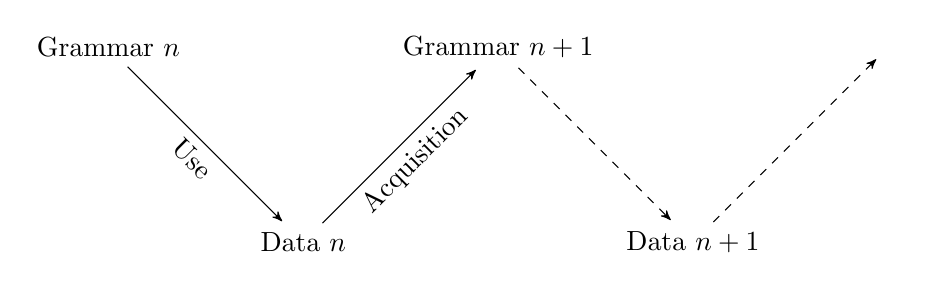
\begin{tikzpicture}[->,>=stealth',shorten >=1pt,auto,node distance=3.5cm]
      \node (A)      {Grammar $n$};
      \node (B) [below right of=A]  {Data $n$};
      \node (C) [above right of=B] {Grammar $n+1$};
      \node (D) [below right of=C] {Data $n+1$};
      \node (E) [above right of=D] {};
      \path[->] (A)  edge node[sloped, anchor=center, below] {Use} (B)
      (B) edge node[sloped, anchor=center, below] {Acquisition} (C)
      (C) edge[dashed] node {} (D)
      (D) edge[dashed] node {} (E);
    \end{tikzpicture}
  \end{center}
\caption{The iterated process of language change through acquisition and use}
\label{change-labeled}
\end{figure}


At the center of this endeavor will be a diachronic process that implicates both use and acquisition, the development in the expression of sentential negation over time known as \emph{Jespersen's cycle} \citeyearpar{jespersen:1917}. The process is often described as the result of two transitions. The first transition occurs when a preverbal form of negation is replaced by an embracing form, which is initially characterized as being more emphatic. The second transition occurs when this embracing form is subsequently replaced by a purely postverbal form. In the history of English, we observe both of these two transition in Middle English from \emph{\textcolor{red}{ne}} to \emph{\color{blue} ne...not} and from \emph{\color{blue} ne...not}  to \emph{\color{green} not}. Our goal will be to determine the role of use and acquisition in each of these transitions.

In Chapter 2 we begin by distinguishing between two phenomena that have often been conflated in investigations of Jespersen's cycle. In particular, we argue that Jespersen's cycle as it is often described consists of both a \emph{formal} and a \emph{functional cycle}. The formal cycle describes the change in the formal complexity of negation over time. It takes place as negation becomes more and then less formally complex, as can be seen in the transitions in the history of English from \emph{\textcolor{red}{ne}} to \emph{\color{blue} ne...not}  to \emph{\color{green} not}. The functional cycle describes the way that different forms of negation are used to signal meaning. It takes place as one form of plain negation  is replaced by another form. This can be seen in the history of English from \emph{\textcolor{red}{ne}} to \emph{\color{blue} ne...not} where the originally empathic \emph{\color{blue} ne...not} displaces \emph{\textcolor{red}{ne}} as it increases in frequency, loses its emphasis, and comes to signal plain negation. We note the logical and empirical relationship between the two cycles: the functional cycle can occur independently of the formal cycle. This result informs the structure of the rest of the dissertation; we start by addressing the functional cycle before turning to the formal cycle.

The first part of this dissertation addresses the functional cycle. In Chapter 3 we introduce the mathematical tools we will use to model the functional cycle. In particular, we show how we can use evolutionary game theory to describe how meaning is signaled in a population over time. Importantly, these tools allow us to model  a qualified kind of Gricean rationality. That is, individuals are \emph{boundedly rational} insofar as they have limited cognitive and informational resources \citep{simon1955,simon1957}. Yet, these tools allow us to show how the actions of individuals can give rise to change at the population level, even when those small decisions are not the product of conscious deliberation \citep{Keller:1994}. This is particularly important when we turn to the functional cycle in Chapter 4, where we show that the first transition from \emph{\textcolor{red}{ne}} to \emph{\color{blue} ne...not} can be explained as the result of speakers' limitations in keeping track of common versus private knowledge.  So, just as Gricean rationality has been used to explain particular patterns of synchronic use, a kind of bounded rationality allows us to explain the functional cycle. So, how we use these two forms explains why they change over time, and the transition from  \emph{\textcolor{red}{ne}} to \emph{\color{blue} ne...not}. 

However, the same model does not apply to the transition from \emph{\color{blue} ne...not}  to \emph{\color{green} not}, so we turn to the formal cycle in the second part of this dissertation. In Chapter 5 we describe a model of syntactic acquisition and determine its predictions for both of the transitions of the formal cycle. In particular, we show that acquisition cannot explain either of the two transitions from  \emph{\textcolor{red}{ne}} to \emph{\color{blue} ne...not} or  from \emph{\color{blue} ne...not}  to \emph{\color{green} not}, other than as the result of a random change in the grammars acquired. In Chapter 6 we test this possibility using statistical methods developed in population genetics to test for random drift versus selection. We find that we can reject random drift in the case of the first transition from \emph{\textcolor{red}{ne}} to \emph{\color{blue} ne...not}, but we cannot reject drift in the case of the second drift from \emph{\color{blue} ne...not}  to \emph{\color{green} not}. This first result suggests that use is the driving force behind the first transition as part of the functional cycle. The second result shows that acquisition does not play a role in any of the observed transitions.  So, insofar as we can offer an explanation of either of the observed changes, we need the notion of pragmatic competence to do so.

%\section{Language Change}
%
%\begin{itemize}
%	\item Language undoubtedly changes
%	\item Weinreich, Labov, Herzog: constraints but not transition or actuation
%	\item What constitutes change? Mental representations
%\end{itemize}
%
%
%A ..theory" of language change in the rigorous sense can be visualized in a relatively strong form and in a weak form. In its strong form, the theory would predict, from a description of a language state at some moment in time, the course of development which that language would undergo within a specified interval. Few practising historians of language would be rash enough to claim that such a theory is possible. In a more modest version, a theory of language change would merely assert that every language constantly undergoes alteration, and it would formulate constraints on the transition from one state of a language to an immediately succeeding state. It might predict further that no language will assume a form in violation of such formal principles as are postulated to be universal in humnan languages. Without predicting positively what will happen (except that the language will somehow change), such a theory would at least assert that some changes will not take place. WLH p.99
%
%The problem of constraints on immediately succeeding language states, to which we alluded above, is in our view subsumed under the broader theoretical question. Of course, we too want to inquire into the set of possible changes and possible conditions for changes which can take place in a structure of a given type. Nor do we want to dismiss the transition problem: it remains entirely relevant to ask about intervening stages which can be observed, or which must be posited, between any two forms of a language defined for a language community at different times. But if the theory is to be illuminating with respect to recorded histories of languages, we must ask two further questons: How are the observed changes embedded in the matrix of linguistic and extralinguistic concomitants of the forms in question? (That is, what other changes are associated with the given changes in
%a manner that cannot be attributed to chance?) And how can the observed changes be evaluated in terms of their effect upon linguistic structure, upon communicative efficiency (as related, e.g., to functional load), and on the wide range of nonrepresentational factors involved in speaking? WLH p.101
%
%\section{Linguistic Explanation}
%
%\begin{itemize}
%	\item Causality : necessary and sufficient conditions
%	\item What counts as an explanation?
%	\item Chomsky: Observational, Descriptive, Explanatory adequacy (Van Frassen: Deductive)
%	\item Description alone is not enough!
%	\item What counts as an explanation in Linguistics?
%\end{itemize}
%
%\section{Causal Forces}
%
%\begin{itemize}
%	\item Need additional evidence that description is grounded in reality somehow.
%	\item We can't rewind and redo language experiments!
%	\item We can note the falsifying cases
%%	\item Stochastic vs deterministic processes
%%	\item Mean dynamics
%\end{itemize}
%
%Languages change. 
%
%Or rather, the mental representations that characterize knowledge change. Somewhere along the iterated chain of language transmission, from one generation to the next, the content of what is learned is substantially different. 
%
%Language change is evidenced by a difference between the linguistic expressions of one generation and the next. Given that the output from one generation serves as the input to the next, both language acquisition and use are crucial to the process of change. While the input to acquisition arises from the interplay of many factors, it is not arbitrary. Rather, it is governed by a \emph{pragmatic competence} that ``underlies the ability to use [\emph{grammatical competence}] along with the conceptual system to achieve certain ends or purposes'' \citep[59]{chomsky1980rules}. In the terms of \cite{chomsky1986knowledge}, the process of language acquisition maps the \emph{E-Language} of one generation to the \emph{I-Language} of the next, whereas pragmatic competence is what governs the mapping from each generation's \emph{I-Language} to its \emph{E-Language}.
%
%In the Gricean tradition \citep{Grice:1975,Levinson:1983, Horn:1984}, this pragmatic competence has been framed in terms of speakers' beliefs, preferences, and intentions. Linguistic expressions are used according to a \emph{Cooperative Principle} whereby interlocutors are taken to make the appropriate contribution to the conversation at the appropriate time towards ``the accepted purpose or direction of the talk exchange'' \citep[26]{Grice:1975}. This framework deftly captures the systematic relationship between what is \emph{said} and what is \emph{meant}, but is clearly an idealization: speakers and hearers might, but need not have the same preferences or goals in a given exchange.   This dissertation aims at understanding the consequences of loosening the assumption of Gricean commonality. It will examine how differences in speakers' and hearers' preferences might impact the use and acquisition of linguistic signals over time. 
%
%At the center of this endeavor will be a diachronic process that implicates both use and acquisition, the development in the expression of negation over time known as \emph{Jespersen's Cycle} \citeyearpar{jespersen:1917}. The main components of this dissertation address the main components of the cycle in turn. First, we consider how the expression of negation transitions from a purely preverbal negator with an optional \emph{emphatic} postverbal element towards a system with obligatory preverbal and postverbal elements. We present a formal model that derives this transition from even a slight preference for exaggeration on the part of speakers. If speakers prefer hearers' response to the emphatic form, then the optional postverbal element will increase in use. On the way up it experiences a kind of \emph{rhetorical devaluation} \citep{dahl:2001}, and is at least partially \emph{bleached} of its emphatic force because, simply put, to ``to emphasize everything is to emphasize nothing'' \citep{kiparsky-condoravdi:2006}. Second, we consider how the expression of negation can shift from the original preverbal negator to the new, increasingly-used, postverbal element. We outline the conditions under which a learner would posit that the postverbal element is a negator in its own right. If the preverbal element appears in contexts where it does not itself express negation, this provides evidence that postverbal element expresses negation and for the eventual loss of the preverbal element entirely. We consider the interaction between these two components of the cycle.
%
%The main contributions of this line of research are the following. First,  it extends recent work in game-theoretic pragmatics that has begun to explore the broader space of possibly divergent preferences \citep{benz-jager-van-rooij:2006, franke:2008, franke-etal:2012, de-jaegher-van-rooij:2013}. This can be taken as a straightforward generalization of the Gricean program to understand the use of linguistic expressions not just as something ``all or most do \emph{in fact} follow but as something that it is \emph{reasonable} for us to follow, that we \emph{should not} abandon'' \citep[29]{Grice:1975}.  Second, it incorporates this perspective into the use of linguistic signals over time. In particular, it suggests how Grice's criterion of reasonability might cut both ways: there are some patterns of use that we \emph{should} and \emph{do} abandon. Differentiating the cases where we expect stability from those where we expect change adds to a broader causal theory of language change \citep{yang2000internal}. 
%
%
%Namely, it offers an additional \emph{internal} force of language change, which derives from a shared pragmatic competence. In the case of Jespersen's Cycle it suggests how morphosyntactic change might arise through a kind of communicative bleaching.   More broadly, it offers insight into the interaction between use and acquisition implicit in the common representation of iterated language change as in Figure \ref{trans}.
%
%\begin{figure}
%\begin{center}
%\begin{tikzpicture}[->,>=stealth',shorten >=1pt,auto,node distance=3cm]
%  \node (A)      {Grammar $n$};
%  \node (B) [below right of=A]  {Data $n$};
%  \node (C) [above right of=B] {Grammar $n+1$};
%  \node (D) [below right of=C] {Data $n+1$};
%  \node (E) [above right of=D] {};
%\path[->] (A)  edge node {} (B)
%  (B) edge node {} (C)
%  (C) edge node {} (D)
%  (D) edge[dashed] node {} (E);
%\end{tikzpicture}
%\end{center}
%\caption{The iterated process of language change through acquisition and use}
%%\label{trans}
%\end{figure}
%
%
%\begin{figure}
%  \begin{center}
%    \begin{tikzpicture}
%      \node (left)      {\includegraphics[width=.15\textwidth]{left.jpg}};
%      \node (right) [right=4cm  of left] {\includegraphics[width=.1\textwidth]{right.jpg}};
%      \node (G1) [draw,above=.25cm of left] {Grammar $n$};
%      \path[->] (left)  edge[dashed, out=-35,in=215] node[below]  {Data $n$} (right);
%      \node (G2) [draw,above=.25cm of right] {Grammar $n+1$};
%    \end{tikzpicture}
%  \end{center}
%	\caption{}
%%	\label{acquisition}
%\end{figure}
%
%
%\begin{figure}
%  \begin{center}
%    \begin{tikzpicture}
%      \node (left)      {\includegraphics[width=.15\textwidth]{left.jpg}};
%      \node (right) [right=4cm  of left] {\includegraphics[width=.15\textwidth]{right.jpg}};
%      \node (G1) [draw,above=.25cm of left] {Grammar $n$};
%      \node (G2) [draw,above=.25cm of right] {Grammar $n$};
%      \path[->] (left)  edge[dashed, out=-35,in=220] node[below]  {Data $n$} (right);
%      \path[->] (right)  edge[dashed, out=215,in=-40] (left);
%    \end{tikzpicture}
%  \end{center}
%	\caption{}
%	\label{use}
%\end{figure}
%
%
%\begin{figure}
%  \begin{center}
%    \begin{tikzpicture}[->,>=stealth',shorten >=1pt,auto,node distance=3cm]
%      \node (A)      {Grammar $n$};
%      \node (B) [below right of=A]  {Data $n$};
%      \node (C) [above right of=B] {Grammar $n+1$};
%      \node (D) [below right of=C] {Data $n+1$};
%      \node (E) [above right of=D] {};
%      \path[->] (A)  edge node[sloped, anchor=center, below] {Use} (B)
%      (B) edge node[sloped, anchor=center, below] {Acquisition} (C)
%      (C) edge[dashed] node {} (D)
%      (D) edge[dashed] node {} (E);
%    \end{tikzpicture}
%  \end{center}
%\caption{The iterated process of language change through acquisition and use}
%\label{change-labeled}
%\end{figure}
%
%
%
%
%
%The rest of the proposal is structured as follows. Section \ref{Background} offers an overview of Jespersen's Cycle.  We consider the two major approaches to the change, as a \emph{pull-chain} or a \emph{push-chain}. We adopt the latter given that the driving force behind the cycle appears to be pragmatic in nature, stemming from continuous loss and renewal of emphatic negation. We then consider a natural simplification of Eckardt's \citeyear{eckardt2006} analysis of emphatic negation. In Section \ref{Signaling} we develop the mathematical framework that will be used to explicitly connect the analysis of emphatic negation with the cycle. In Section \ref{Cycles} we apply the framework and consider the cycle as a signaling game played in a population where the interests of speakers and hearers slightly diverge. We determine the conditions for the existence of different kinds of equilibria, and the impact of the introduction of new signals under the game dynamics. Finally, in Section \ref{Stability} we 
%determine how the change brought about by use might impact acquisition over time. We suggest different mechanisms that might impact the amount of evidence available to learners at various points in time and how this shapes the trajectory of the change.
%
%\begin{quote}
%	   I am, however, enough of a rationalist to want to find a basis that underlies these facts, undeniable though they may be; I would like to be able to think of the standard type of conversational practice not merely as something that all or most do \textbf{in fact} follow but as something that it is \textbf{reasonable} for us to follow, that \textbf{we should not abandon}. 
% \end{quote}           
%
%\begin{quote}
%As one of my avowed aims is to see talking as a special case or variety of purposive, indeed rational, behaviour, it may be worth noting that the specific expectations or presumptions connected with at least some of the foregoing maxims have their analogues in the sphere of transactions that are not talk exchanges. (Grice 1989, p. 28)
%\end{quote}
%
%\begin{quote}
%[T]o say what a word means in a language is to say what
%it is in general optimal for speakers of that language to
%do with that word, or what use they are to make of it;
%what particular intentions on particular occasions it is
%proper for them to have. Of course, there is no
%suggestion that they always have to have those
%intentions: it would merely be optimal, ceteris paribus,
%for them to have them. (Grice, 1989, p. 299)
%\end{quote}
%
%\begin{quote}
%The maxims do not seem to be coordinate. The maxim
%of Quality [...] does not seem to be just one among a
%number of recipes for producing contributions; it seems
%rather to spell out the difference between something�s
%being, and (strictly speaking) failing to be, any kind of
%contribution at all. False information is not an inferior
%kind of information; it just is not information. (Grice,
%1989, p.371)
%\end{quote}
%
%Conflicts of interest play markedly different roles in Linguistics and Biology. On the one hand, Gricean pragmatics has aimed at understanding the inferences that a listener can draw from a speaker's contribution on the explicit assumption of a shared set of purposes for an exchange. On the other hand, animal signaling has aimed at understanding the existence and persistence of signaling systems in the face of varying degrees of inter- and intra-species conflict.  Both endeavors hinge on the role of conflict, either in its presence or absence. Yet, in the abstract, both deal with the transmission and interpretation of signals. This leads us to consider what happens when we extend our linguistic considerations beyond perfectly aligned interests. 
%
%At first glance, this step outside the idealized realm of common causes yields some forbidding results: conflicts of interest erode communication. The following reasoning, familiar from biological studies of animal signaling, makes clear the root of this unraveling \citep{searcy-nowicki:2005}. Imagine two agents: a sender who sends a signal and a receiver who receives the signal. Suppose that the sender has no incentive to be truthful, in fact, let us suppose that he has every incentive to deceive the receiver. If the sender has an incentive to deceive, then the receiver should not listen. If the receiver does not listen, then the sender has no motive to signal in the first place. Crucially, the actions of the sender depend on those of the receiver and vice versa. Given this interdependence, conflicting interests undermine the information conveyed by signals, rendering them, so to speak, meaningless. 
%
%The same reasoning holds in the case of an entire population of senders and receivers interacting over time. Senders will learn or evolve to dissimulate and receivers will learn or evolve to distrust. This process takes on the familiar form of the \emph{tragedy of the commons} \citep{hardin:1968}. Individuals will always be tempted to exploit the common resource of credulity. Collectively, this incentive to exploit exhausts the resource. Only a fool would tell the truth when there is something to be gained from deception, and only a fool would trust others to be truthful. 
%
%
%\begin{quote}
%	   Make your conversational contribution  such as is required, at the stage at which it occurs, by the accepted purpose or direction of the talk exchange in which you are engaged. One might label this the \textbf{Cooperative Principle}.
%\end{quote}           
%
%
%Silence, or at best meaningless babble, is the equilibrium state in the population: neither senders nor receivers have reason to unilaterally change their behavior. Thomas Schelling's grim pronouncement comes to mind \citep[26]{schelling:1978}:  
%
%\begin{quote}
% The body of a hanged man is in equilibrium when it finally stops swinging, but
%nobody is going to insist that the man is all right.
%\end{quote}
%This sentiment holds doubly. Not only is the inability to convey information problematic, but, we do actually observe informative signaling. The existence of such signaling despite conflicting interests is a genuine puzzle. 
%
%This problem was not lost on Grice, insofar as he recognized the fundamental
%role of his \emph{Maxim of Quality} to the entire enterprise.
%
%\begin{quotation}
%It is obvious that the observance of some of these maxims is a matter of less urgency than is the observance of others; a man who has expressed himself with undue prolixity would, in general, be open to milder comment than would a man who has said something he believes to be false...[O]ther maxims come into operation only on the assumption that this maxim of Quality is satisfied \citep[27]{Grice:1975}
%\end{quotation}
%
%Yet, while we have every incentive to abide by the maxim of Quality when it serves our interests, we have every reason to do otherwise when it does not. So, what keeps human language from the downward spiral to silence? In this regard we can look to animal communication where much work has been devoted to explaining the evolutionary stability of communication. In large part, these solutions take the form of different mechanisms that mitigate conflicts of interest between senders and receivers. 
%
%For example, a sender might guarantee his commitment to the truth by incurring a sufficiently high cost to send a signal. This \emph{handicap principle}  \citep{Zahavi:1975} allows for stable signaling despite conflicting interests.\footnote{See \cite{maynard-smith-harper:2004} and \cite{searcy-nowicki:2005} for thorough discussions of handicaps in animal signaling. Also,\cite{grose:2011} offers a concise but useful discussion of the history and details of the handicap principle. In the economic tradition, \cite{spence:1973} develops a parallel model for educational attainment as a costly signal of job suitability.} To take the usual example, a peacock incurs a cost for his magnificent tail: significant metabolic resources are required to develop the tail, and once developed, his ability to fly is hampered and it makes him more conspicuous to predators. But, successfully bearing the tail serves as a signal of his genetic worth. A weaker peacock would not have been able to support the tail and avoid becoming 
%something else's lunch. Thus, potential mates  can take the tail as a signal of a a truly fit peacock. 
%
%When we turn our attention to language, this sort of mechanism need not be appropriate.  In fact, the notion that truthfulness is enforced by cost is problematic: truth tellers expend as much effort learning and producing their language as liars, and no more. As we say, talk is cheap. There are, of course, various alternatives to handicaps that are appropriate for the case of language \citep{scott-phillips:2008}. A particularly appealing alternative given the social nature of humans, and language, is that of reputation. The minimal requirements for a reputation are the ability of agents to recognize each other individually, keep track of past interactions, and condition future behavior on the outcome of those interactions \citep{Trivers1971}. In the long run, the immediate benefits of deception might not be worth the consequences of a bad reputation.
%
%Abstracting away from the details of the actual mechanisms that mitigate conflict, we can consider three general questions.  First, how effective are these mechanisms in aligning the interests of senders and receivers? Given that language exists, such mechanisms are clearly sufficient to stave off total collapse. However, given that signals are not always used in accordance with the Maxim of Quality, such mechanism are not sufficient to ensure the idealized case of Gricean commonality. Second, if language is indeed subject to a host of competing pressures, what impact will this have on how linguistic signals are used over time?  If not a tragedy of the commons, might we find a lesser \emph{tragedy of the conversation} where particular signals, but not the system as a whole, are destabilized? Third, do we find instantiations of the predicted patterns of language use? In what follows, these second two question will be our chief concern. 
%
%\section{Roadmap}
%
%\begin{enumerate}
%	\item In Chapter \ref{jespersens-cycle} we outline....
%	\item In Chapter \ref{evolutionary-game-theory} we...
%	\item In Chapter \ref{Cycles} we ...
%	\item in Chapter \ref{learning-theory} we...
%	\item in Chapter \ref{Stability}
%	\item in Chapter \ref{conclusion} we summarize our results.
%\end{enumerate}�



% Jespersen's Cycle
\chapter{Jespersen's Cycles}
\label{jespersens-cycles}

\setlength{\epigraphwidth}{.9\textwidth}
\epigraph{The history of negative expressions in various languages makes us witness the following curious fluctuation: the original negative adverb is first weakened, then found insufficient and therefore strengthened, generally through some additional word, and this in its turn may be felt as the negative proper and may then in course of time be subject to the same developments as the original word. \citep[4]{jespersen:1917}}

Originally coined by \cite{dahl:1979}, the term \emph{Jespersen's cycle} is often used in reference to the observation cited above. It is certainly the most quoted aspect of Jespersen's \citeyearpar{jespersen:1917} seminal work, which prefigures many of the current empirical and theoretical issues in the study of negation (cf. \citealt{horn:1989}). Yet, this passage is also interpreted in two very distinct ways. This fundamental ambiguity stems from the fact that Jespersen noted both \emph{formal} and \emph{functional} patterns in the expression of sentential negation over time.\footnote{Sentential negation refers to the semantic property of negating an entire proposition, not just some subpart. It can be distinguished from morphological (e.g. \emph{un-}, \emph{non-}) and constituent negation (e.g. \emph{John might have not understood}) using several diagnostics such as tag questions \citep{klima1964}  and performative paraphrases \citep{payne1985}. Sentential negation is also distinct from but related to the syntactic notion of standard negation \citep{miestamo2005}, which refers to constructions that can reverse the truth value of a proposition.} Both patterns can be conceived of as cycles in their own right. That is, we can find a series of transitions from and back to states that are in some sense formally or functionally equivalent. But, the term Jespersen's cycle is often used in one of these two senses or the other, without clear distinction. 

%There are a range of ways to analyze the syntactic structures underlying the formal cycle. As summarized in part by \cite{vanderAuwera2009}, different analyses have suggested varying levels of detail in the number and realization of stages, ranging from three stages  \citep{burridge1983,bernini-ramat1996,haspelmath1997,frisch1997,zanuttini1997,horn:1989,hoeksma1997,horn2001,roberts-roussou2003,vanderAuwera-neuckermans2004,mazzon2004,willis2005,lucas2007,jager2008,wallage2008}, to four stages \citep{dahl:1979,posner1985,schwegler1988,schwegler1990,ladusaw1993,schwenter2005,schwenter2006}, up to five stages \citep{honda2000,beukema1999,vanderAuwera-neuckermans2004,zeijlstra2004}.  


Perhaps even worse, the canonical presentation of what is referred to as Jespersen's cycle conflates these two uses \citep{posner1985,schwegler1988,schwegler1990,ladusaw1993,schwenter2005,schwenter2006}. Where parentheses at the second stage indicate an optional post-verbal element that is characterized as being emphatic, the following stages are posited.

\begin{center}
\begin{enumerate}
     \item \textsc{\textcolor{red}{neg V}}
    \item  \textsc{\textcolor{red}{neg V} \textcolor{blue}{(neg)}}
    \item \textsc{\color{blue} neg V neg}
    \item \textsc{\color{green} V neg}
\end{enumerate}
\end{center}
This chapter is devoted to defining and distinguishing the two uses of the term intertwined in this representation, which we will call the formal and functional Jespersen cycles. In short, the distinction is between changes in the forms of negation available and changes in how those forms are used to signal meaning, respectively.  Our goal is to clarify the relationship between the two cycles and what would count as an explanation of each.

First, we outline the formal aspects of how negation is expressed at the stages of the formal cycle. We provide a historical description of the structural forms that express negation at different points in the history of English, and compare this trajectory with that of French to emphasize particular aspects of the formal cycle. Second, we outline the function of those forms at different stages of the functional cycle. We provide a historical description of the functions of the different forms at points in the history of both English and French, noting the relationship between optionality and these different functions. We also note the logical relationship between the two cycles: the formal cycle entails the functional cycle, but not vice versa. Third, in light of our definitions and the logical relationship between the two cycles, we discuss two ways of conceptualizing the causes of the cycles and the potential role of syntactic acquisition and pragmatic use in both. 

While the main motivation of this chapter is terminological, distinguishing between the two kinds of cycles has an important consequence. Given the logical relationship between the two cycles, an explanation of the formal cycle requires an explanation of the functional cycle. This informs the structure of the dissertation. Since an explanation of the functional cycle must be our first priority, we begin in Part I by pursuing such an explanation. In Chapter 3 we present a mathematical framework for understanding how different functional meanings are signaled in populations over time. In Chapter 4 we apply this framework to model the functional cycle in the history of English.  With this in place, in Part II we turn to the formal cycle. In Chapter 5 we evaluate a model of syntactic acquisition and the role it might play in an explanation of the formal cycle. In Chapter 6 we consider the possibility that stochastic processes may lead to the transitions in the formal cycle. So, our goal in this chapter is to set the foundation for the rest of the dissertation by clarifying the distinction between the two kinds of cycles.


\section{The formal cycle}

The formal cycle is defined in terms of the forms that are used to express negation over time, and consists of two transitions. At the start of the formal cycle, a single element is used to express negation. The first transition occurs when this single element is supplemented by additional lexical material. The second transition occurs when the original negative element is subsequently lost, leaving the added lexical material as the only expression of negation. In the most general sense, the formal cycle occurs when the form of negation becomes more and then less complex.  It is cyclic in the sense that the forms of negation at the start and end of the cycle are of equal formal complexity. 

This can be shown schematically as in Figure \ref{formal-cycle}, where the vertical axis represents the degree of formal complexity. The first transition takes place from \circled{1} to \circled{2} with the addition of material. The second transition takes place from \circled{2} back to \circled{1} with the loss of material. The addition of material leads to an increase in formal complexity of negation and the loss of material leads to a decrease. The formal cycle is then just a cycle from and back to a less complex form of negation: negation is expressed by some stuff, then more stuff, then less stuff.

%\footnote{We could perhaps be a bit more general by replacing one and two in Figure \ref{formal-cycle} with \circled{$n$} and \circled{$n+1$}, respectively, where $n$ indicates the number of elements used to express negation.} 

\begin{figure}
% Modified from:
% A simple cycle
% Author : Jerome Tremblay
\begin{tikzpicture}
	% Define margin to offset
	\def \margin {8}
	% Draw nodes
	\node[draw,circle] at ({90}:3) {2};
	\node[draw,circle] at ({270}:3) {1};
	% Draw arcs
	\draw[->, >=latex] ({270 - \margin}:3) arc ({270 - \margin}:{90 + \margin}:3);
	\draw[->, >=latex] ({90 - \margin}:3) arc ({90 - \margin}:{-90 + \margin}:3);
	% Draw complexity axis
	\draw[->, >=latex] (-5,-3) -- (-5,3);
	\node[align=center,text width=2cm] at (-6.25, 0) {Formal complexity};
\end{tikzpicture}
\caption{The formal Jespersen cycle}
\label{formal-cycle}
\end{figure}

For example, Jespersen noted that in the history of several European languages, including English and French, a pre-verbal negative element is supplemented by a post-verbal element, and the pre-verbal element is subsequently lost.  This can be shown schematically as in Figure \ref{formal-cycle-spiral} where the different forms of negation are arranged according to formal complexity on the vertical axis and time along the horizontal axis. At both the start and the end of the formal cycle a single element expresses negation. Intuitively, if we abstract away from the structural realization of the forms as pre- or post-verbal, then Figure \ref{formal-cycle-spiral} maps onto Figure \ref{formal-cycle}. The curious fluctuation in form that Jespersen noted simply becomes a closed orbit through the space of formal complexity.

\begin{figure}
\begin{center}
\begin{tikzpicture}[->,>=stealth',shorten >=1pt,auto,node distance=3cm]
  \node (A)      {\textsc{\textcolor{red}{neg V}}};
  \node (B) [above right of=A]  {\textsc{\color{blue} neg V neg}};
  \node (C) [below right of=B] {\textsc{\color{green} V neg}};
  \node (D) [left of=A] {};
  \node (E) [above of=D] {};
\path[->] (A)  edge node {} (B)
  (B) edge node {} (C);
	% Draw axes
    \draw[->] (-1.5,0) -- (-1.5,2);
  \node[align=center, text width=2cm] at (-2.75, 1) {Formal complexity};
    \draw[->] (0,-1) -- (4,-1);
    \node at (2,-1.5) {Time};
\end{tikzpicture}
\end{center}
\caption{The realization of the formal cycle in English and French}
\label{formal-cycle-spiral}
\end{figure}

We see the first stage of the formal cycle in the history of English with the pre-verbal \emph{\textcolor{red}{ne}} in Old English, which expresses sentential negation alone.

\exg. Ic \textcolor{red}{ne} secge\\
      I \textsc{neg} say\\
      (Old English)


This is followed by a stage of embracing or bipartite negation where a post-verbal negative element is added. This is seen in Middle English, where \emph{\textcolor{blue}{ne}} is supplemented by \emph{\textcolor{blue}{not}}.


\exg. I \textcolor{blue}{ne} seye \textcolor{blue}{not}\\
      I \textsc{neg} say \textsc{neg}\\
      (Middle English)

There are several sources that these additional elements are drawn from, most notably from \emph{negative polarity items}, overwhelmingly the set of \emph{minimizers} (e.g. ``not a drop'', ``not a hair'') and \emph{generalizers} (e.g. ``not ever'', ``not at all'', \citealt{horn:1989}). For example, in the case of English, \emph{not} comes from Old English \emph{nawiht} (\emph{literally} ``no thing, creature, being''). Other sources include, indefinite pronouns (e.g. ``no one''), negative adverbs (e.g. ``never'', cf. \citealt{horn:1989,vanGelderen2008negative}), negative verbs (e.g. ``refuse", ``deny", ``reject", ``avoid", ``fail", and ``lack",  \citealt{givon1978}), and the concatenation of negative and existential verbs \citep{croft1991}.


In light of this broad range of sources, it is important to note that the first transition need not consist of the addition of a post-verbal element. For example, in modern African American Vernacular English, negation can be supplemented by a pre-verbal element \emph{eem}, which can express negation in its own right \citep{jones2015}.

\ex. You do\textcolor{blue}{n't eem} know.

\ex. You \textcolor{blue}{eem} know.

As \cite{jones2015} notes, this form comes from but is arguably distinct from \emph{even}.

\ex.  \# \textcolor{blue}{eem} numbers

Importantly, it is the formal status rather than the structural position that is relevant. Given the range of sources for additional negative elements, this is not surprising.  But, it bears emphasis that the transition from pre- to post-verbal negation is not the only path through the formal cycle.  The transition could just as well have been from post- to pre-verbal negation or from and back to pre-verbal negation. It is a contingent historical fact, arising from the syntax of  English and the source of the additional  material, rather than some necessary property of the formal cycle. 

The final stage in the formal cycle is a return to a single negative element. This is seen in Early Modern English, where the preverbal element in \emph{\textcolor{blue}{ne...not}}  is lost, leaving the post-verbal \emph{\textcolor{green}{not}}  as the sole negative element.

\exg. I say \textcolor{green}{not}\\
      I say \textsc{neg}\\
      (Early Modern English)

The emergence of  \emph{do}-support in Early Modern English yields a state parallel to Old English with a sole pre-verbal negator:

\exg. I do \textcolor{red}{not} say\\
      I do \textsc{neg} say\\
      (Present-day English)

The contraction of negation offers an even closer parallel to Old English where \emph{ne} contracted with several verbs (e.g. \emph{ne be} $\rightarrow$ \emph{nis}).

\exg. I do\textcolor{red}{n't} say\\
      I do-\textsc{neg} say\\
      (Present-day English)

But, however suggestive these further developments are, they are not necessary components of the formal cycle.  \citet[10]{jespersen:1917} himself noted the uniqueness of these developments, which he attributed to a tendency to place negation at the beginning of the sentence to avoid confusion. As he put it, the effect of post-verbal negation in German results in a kind of semantic garden path.\footnote{Living is not the highest good (lit. The living is the good highest not)}

\begin{quote}
[T]he hearer or reader is sometimes bewildered at first and thinks that the sentence is to be understood in a positive sense, till suddenly he comes upon the \emph{nicht}, which changes everything; see, for instance ``Das leben ist der g\"{u}ter h\"{o}chstes nicht."
\end{quote}
Yet, despite this purported tendency, the majority of languages that Jespersen noted, including his native Danish, persist in a perplexing state of post-verbal negation. This can only be taken as further evidence that we ought to interpret the implications of Jespersen's observation in formal rather than structural terms. It matters how much stuff is used to express negation, not where that stuff is.

% The transition from purely post-verbal to purely pre-verbal negation is certainly not necessary. For example, German went through a formal cycle in (cf. CHECK \cite{jager2008}), but negation remains purely post-verbal.

% \footnote{The increasing preference of n't over not in colloquial use is illustrated by the use of not contractions of American presidents from Kennedy to Bush. While Kennedy and Nixon still used the uncontracted form not in the majority of cases (during public debates), Bush Sr. and Clinton used this form in only in 14-17\% of all cases (Yaeger-Dror \& Hall-Lew (2002)}

Given the stages of the formal cycle in the history of English, it is useful to give them some historical context. The stages are summarized in Figure \ref{english-timeline}. The horizontal axis represents years in the common era. Immediately above the horizontal axis are commonly-used terms for historical periods: Old English (\emph{ca.} 400-1175 CE), Middle English (\emph{ca.}1175-1450 CE), Early Modern English (\emph{ca.} 1450-1650 CE), and Modern English (\emph{ca.} 1650-Present CE). Above these general time periods are the spans of the different forms of negation.  From Old to Early Modern English we make a full formal cycle from and back to a single negative element. We also see the transition at the end of the formal cycle from post- back to pre-verbal negation in Modern English. 

Below the axis are rough historical anchors that offer a general sense of the historical periods: Beouwulf, the Old English epic poem written some time between 700-1050 CE; Chaucer, the Late Middle English author who is widely-credited as the first to write in the vernacular language of his day, from around 1350-1400 CE; and Shakespeare, the noted dramatist and playwright, from around 1550-1650 CE.


\begin{figure}
\resizebox{\linewidth}{!}{% 
     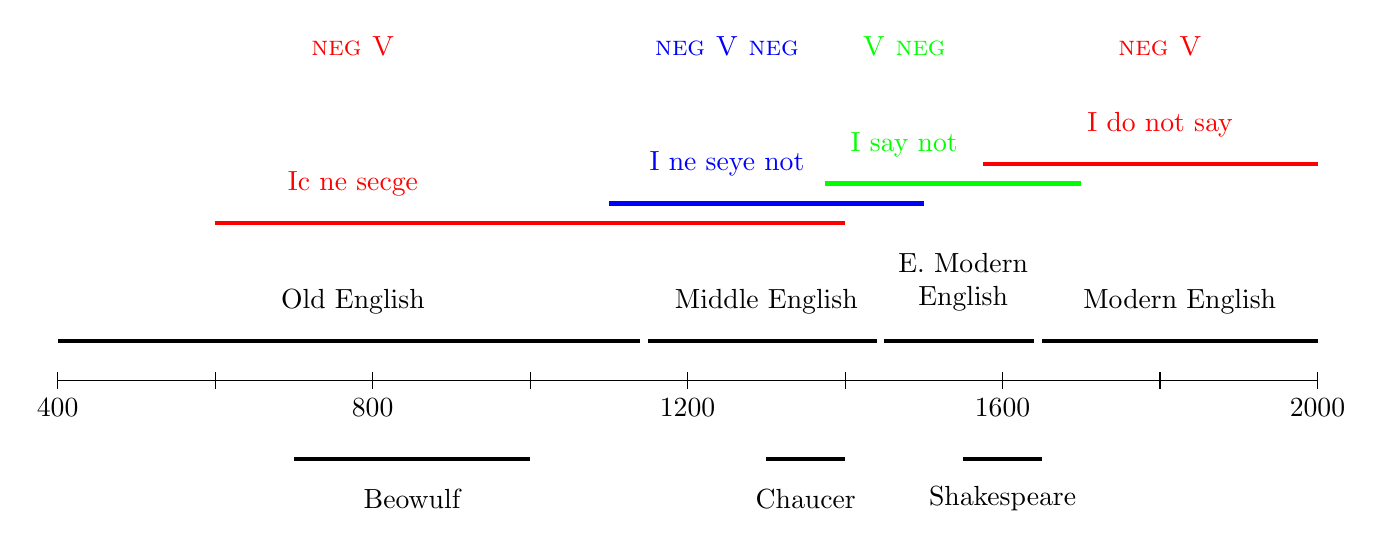
\begin{tikzpicture}
%draw horizontal line
\draw (0,0) -- (16,0);
%draw ticks
\foreach \x in {0, 2, 4, 6, 8, 10, 12, 14, 16}{
   \draw (\x,3pt) -- (\x,-3pt);
}
%draw tick dates
\draw (0,0) node[below=3pt] { 400 } node[above=10pt] { };
\draw (4,0) node[below=3pt] { 800 } node[above=10pt] { };
\draw (8,0) node[below=3pt] { 1200 } node[above=3pt] { };
\draw (12,0) node[below=3pt] { 1600 } node[above=3pt] { };
\draw (16,0) node[below=3pt] { 2000 } node[above=3pt] {  };
% Historical examples
\draw [ultra thick] (3,-1) to (6,-1);
\draw (4.5, -1.5) node {Beowulf};
\draw [ultra thick] (9,-1) to (10,-1);
\draw (9.5, -1.5) node {Chaucer};
\draw [ultra thick] (11.5,-1) to (12.5,-1);
\draw (12, -1.5) node {Shakespeare};
% Add historical languages
% Old English : 400-1175
% Middle English : 1175-1450
% E. Modern English : 1450-1650
% Modern English : 1650-Present
\draw [ultra thick] (0,.5) to (7.4,.5);
\draw (3.75, 1) node {Old English};
\draw [ultra thick] (7.5,.5) to (10.4,.5);
\draw (9, 1) node {Middle English};
\draw [ultra thick] (10.5,.5) to (12.4,.5);
\draw (11.5, 1.25) node[text width=2cm,align=center] {E. Modern English};
\draw [ultra thick] (12.5,.5) to (16,.5);
\draw (14.25, 1) node {Modern English};
% draw ticks for historical examples
% ne 		: 400-1300
% ne..not	: 1100-1400
% not		: 1350-1700
% do not 	: 1500-2000
\draw [ultra thick,red] (2,2) to (10,2);
\draw (3.75, 2.5) node[red] {Ic ne secge};
\draw [ultra thick,blue] (7,2.25) to (11,2.25);
\draw (8.5, 2.75) node[blue] {I ne seye not};
\draw [ultra thick,green] (9.75,2.5) to (13,2.5);
\draw (10.75, 3) node[green] {I say not};
\draw [ultra thick, red] (11.75,2.75) to (16,2.75);
\draw (14, 3.25) node[red] {I do not say};
% draw negative forms
\draw (3.75,4) node [above] {\textsc{\color{red} neg V}};
\draw (8.5,4) node [above] {\textsc{\color{blue} neg V neg}};
\draw (10.75,4) node [above] {\textsc{\color{green} V neg}};
\draw (14,4) node [above] {\textsc{\color{red} neg V}};
\end{tikzpicture}
}
\caption{Timeline of negation in the history of English}
\label{english-timeline}
\end{figure}

The history of negation in French offers a parallel to the formal cycle in English, although the exact details of the timeline are not without dispute (cf. \citealt{martineau-mougeon2003}).  The Old French pre-verbal \emph{\textcolor{red}{ne}} becomes Middle French \emph{\textcolor{blue}{ne...pas}}, and subsequently Modern Colloquial French post-verbal \emph{\textcolor{green}{pas}}.

\exg. Jeo \textcolor{red}{ne} dis\\
      I \textsc{neg} say\\
      (Old French)

\exg. Je \textcolor{blue}{ne} dis \textcolor{blue}{pas}\\
      I \textsc{neg} say \textsc{neg}\\
      (Middle French)

\exg. Je dis \textcolor{green}{pas}\\
      I say \textsc{neg}\\
      (Modern Colloquial French)

Again, it is useful to provide some historical context. The stages of the formal cycle in the history of French are summarized in Figure \ref{french-timeline}. Immediately above the horizontal axis are commonly-used terms for historical periods: Old French (\emph{ca.} 900-1350 CE), Middle French (\emph{ca.}1350-1600 CE), Classical French (\emph{ca.} 1600-1700 CE) , and Modern French (\emph{ca.} 1700-Present CE). Above these general time periods are the spans of the different forms of negation.  From Old to Modern French we make a full formal cycle from and back to a single negative element.

Below the axis are rough historical anchors that offer a general sense of the historical periods: Charlemagne, the first Holy Roman Emperor from 750-800 CE; the Hundred Years' War from roughly 1350-1450 CE; Voltaire, the Enlightenment author and satirist from roughly 1700-1800 CE.


\begin{figure}
\resizebox{\linewidth}{!}{% 
     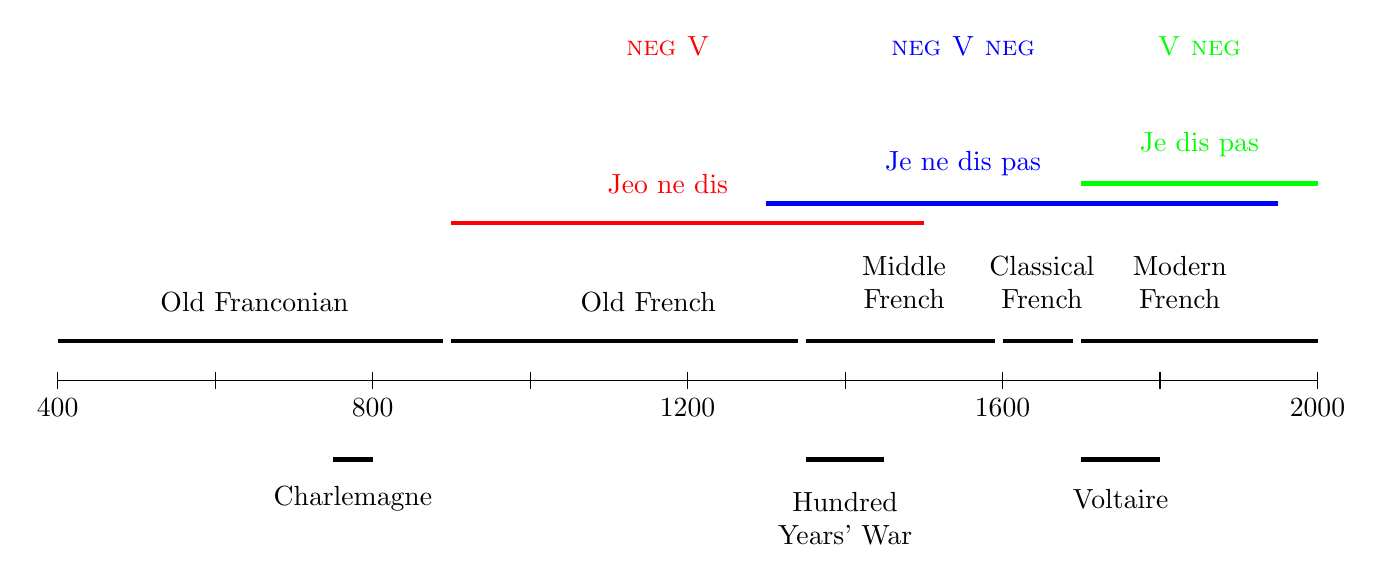
\begin{tikzpicture}
%draw horizontal line
\draw (0,0) -- (16,0);
%draw ticks
\foreach \x in {0, 2, 4, 6, 8, 10, 12, 14, 16}{
   \draw (\x,3pt) -- (\x,-3pt);
}
%draw tick dates
\draw (0,0) node[below=3pt] { 400 } node[above=10pt] { };
\draw (4,0) node[below=3pt] { 800 } node[above=10pt] { };
\draw (8,0) node[below=3pt] { 1200 } node[above=3pt] { };
\draw (12,0) node[below=3pt] { 1600 } node[above=3pt] { };
\draw (16,0) node[below=3pt] { 2000 } node[above=3pt] {  };
% Add historical languages
% Old Franconian : 400-900
% Old French : 900-1350
% Middle French : 1350-1600
% Classical French : 1600-1700
% Modern French : 1700-Present
\draw [ultra thick] (0,.5) to (4.9,.5);
\draw (2.5, 1) node {Old Franconian};
\draw [ultra thick] (5,.5) to (9.4,.5);
\draw (7.5, 1) node {Old French};
\draw [ultra thick] (9.5,.5) to (11.9,.5);
\draw (10.75, 1.25) node[text width=2cm,align=center] {Middle French};
\draw [ultra thick] (12,.5) to (12.9,.5);
\draw (12.5, 1.25) node[text width=2cm,align=center] {Classical French};
\draw [ultra thick] (13,.5) to (16,.5);
\draw (14.25, 1.25) node[text width=2cm,align=center] {Modern French};
% draw ticks for historical examples
% ne 		: 400-1300
% ne..not	: 1100-1400
% not		: 1350-1700
% do not 	: 1500-2000
\draw [ultra thick,red] (5,2) to (11,2);
\draw (7.75, 2.5) node[red] {Jeo ne dis};
\draw (7.75,4) node [above] {\textsc{\color{red} neg V}};
\draw [ultra thick,blue] (9,2.25) to (15.5,2.25);
\draw (11.5, 2.75) node[blue] {Je ne dis pas};
\draw (11.5,4) node [above] {\textsc{\color{blue} neg V neg}};
\draw [ultra thick,green] (13,2.5) to (16,2.5);
\draw (14.5, 3) node[green] {Je dis pas};
\draw (14.5,4) node [above] {\textsc{\color{green} V neg}};
%\draw (14,4) node [above] {\textsc{\color{red} neg V}};
% Historical examples
\draw [ultra thick] (3.5,-1) to (4,-1);
\draw (3.75, -1.5) node {Charlemagne};
\draw [ultra thick] (9.5,-1) to (10.5,-1);
\draw (10, -1.75) node[text width=2.2cm,align=center] {Hundred Years' War};
%\draw [ultra thick] (11,-1) to (12,-1);
%\draw (11.5, -1.5) node {Rabelais};
\draw [ultra thick] (13,-1) to (14,-1);
\draw (13.5, -1.5) node {Voltaire};
\end{tikzpicture}
}
\caption{Timeline of negation in the history of French}
\label{french-timeline}
\end{figure}

\cite{hansen-visconti2009,hansen-visconti2012} note that negation in Louisiana Creole French negation is purely pre-verbal. Of course, this observation comes with the caveat that no conclusions about the future of French can be drawn from this change.

%Although, \cite{hansen-visconti2009,hansen-visconti2012} also note that the post-verbal negator \emph{pas} appears pre-verbally in embedded infinitives \citep{martineau1994}

\exg. Mo \textcolor{red}{pa} di \\
      I \textsc{neg}  say\\
      (Louisiana Creole French)

But again, even if such developments were readily apparent, they would not constitute a necessary component of the formal cycle.
      
Thus, the crucial components of the formal cycle are a transition from one negative element to two, and eventually back to one. For the specific case of English, as well as French, the formal cycle is realized as a transition from pre-verbal to embracing to post-verbal negation. We can represent these transitions schematically as follows.

\begin{center}
\begin{enumerate}
     \item \textsc{\textcolor{red}{neg V}}
    \item \textsc{\color{blue} neg V neg}
    \item \textsc{\color{green} V neg}
\end{enumerate}
\end{center}

Note that these stages are not mutually exclusive. That is, there are transitions between these stages \citep{vanderAuwera2009}.  This captures the theoretical intuition that diachronic change is rarely a dramatic shift. Where parentheses are taken to indicate optionality, the stages can be represented as the following.

\begin{center}
\begin{enumerate}
     \item \textsc{\textcolor{red}{neg V}}
    \item  \textsc{\textcolor{red}{neg V} \textcolor{blue}{(neg)}}
    \item \textsc{\color{blue} neg V neg}
    \item \textsc{\textcolor{blue}{(neg)}  \textcolor{green}{V neg}}    
    \item \textsc{\color{green} V neg}
\end{enumerate}
\end{center}
This more articulated model also comes closer to the diachronic facts. For example, in Late Middle English, all the forms of negation are used contemporaneously: purely pre-verbal, embracing, and post-verbal negation co-occur for a brief period in time. For the moment then, we can take this as the abstract trajectory of the formal cycle over time. 

Importantly, an explanation of the formal cycle in English must consist of two components: it must provide the conditions for the transition from pre-verbal to embracing negation as well as the conditions for the transition from embracing to post-verbal negation. It should be noted that criterion for such explanations can be both qualitative and quantitative. That is, an explanation of the formal cycle can predict both \emph{that} a transition will occur as well as \emph{how} it will occur. In what follows, we will use both kinds of criteria in evaluating models as explanations of change. With this definition of the formal cycle in place, along with what would constitute an explanation for its instantiation in the history of English, we turn to the functional cycle.

%This also occurs synchronically in modern Brazilian Portuguese \citep{schwenter2005, schwenter2006}. 

\section{The functional cycle}

%If the formal cycle is defined by the forms of negation, then the functional cycle is defined by the functions that those forms are put to. It is about how and how many forms are used to mean different things. At the first stage of the cycle one form is generally used to express negation, often characterized as plain negation. Another set of forms is used to express negation in a semantically stronger sense, often characterized as being more emphatic. The first transition in the functional cycle occurs when one of the semantically stronger forms weakens to a strength intermediate between plain and emphatic negation. Thus, at the second stage of the functional cycle the available forms of negation are used to make three functional distinctions. The second transition occurs when the intermediate form weakens even further, coming to have the strength of plain negation, and the original form of plain negation is lost. In the most general sense, the functional cycle occurs when one form of plain negation is replaced by another. It is cyclic in the sense that the number of functionally distinct forms of negation increases then decreases. 

If the formal cycle is defined by the forms of negation, then the functional cycle is defined by the function that those forms are put to. It is about how and how many forms are used to mean different things. At the first stage of the functional cycle a single form is generally used to express negation, often characterized as plain negation. The functional cycle begins with the introduction of another form that is used to express negation in a semantically stronger way, often characterized as being more emphatic. The functional cycle progresses as this new stronger form increases in frequency, weakens, and replaces the original negative form. In the most general sense, the functional cycle occurs when the form of plain negation is replaced by another form. It is cyclic in the sense that the number of functionally distinct forms of negation increases then decreases.

This can be shown schematically as in Figure \ref{functional-cycle} where the vertical axis represents the number of functionally distinct forms of negation. The addition of a new form increases the number of distinctions from \circled{1} to \circled{2}, and the loss of the original form decreases the number of distinctions from \circled{2} back to \circled{1}. However, we should note that Figure \ref{functional-cycle} does not convey all of the necessary information about the functional cycle.

% \footnote{ADD: there aren't JUST two functional distinctions. There are always means of augmenting plain negation to make it emphatic. It might be better to say 2-3-2.}

\begin{figure}
\begin{tikzpicture}
	% Define margin to offset
	\def \margin {8}
	% Draw nodes
	\node[draw,circle] at ({90}:3) {2};
	\node[draw,circle] at ({270}:3) {1};
	% Draw arcs
	\draw[->, >=latex] ({270 - \margin}:3) arc ({270 - \margin}:{90 + \margin}:3);
	\draw[->, >=latex] ({90 - \margin}:3) arc ({90 - \margin}:{-90 + \margin}:3);
	% Draw complexity axis
	\draw[->, >=latex] (-5,-3) -- (-5,3);
	\node[align=center,text width=3cm] at (-6.75, 0) {Functional distinctions};
\end{tikzpicture}
\caption{The functional Jespersen cycle}
\label{functional-cycle}
\end{figure}

Namely, the functional cycle does not hold for just any pair of semantic distinctions. Rather, the incoming form is semantically stronger than the incumbent form. We can more accurately represent the details of the functional cycle as  in Figure \ref{functional-cycle-detail}, where the vertical axis represents semantic strength and the horizontal axis represents time. The original form is supplemented with an additional form that is semantically stronger and this new form weakens over time as it replaces the original from. 

%\footnote{Note that this does not preclude other forms of negation. There are always means for augmenting plain negation to make it emphatic (e.g. `at all', `ever', see \citet[258]{israel2011} and \citet{horn:1989} for incomplete but substantial lists). Crucially the form that is introduced is \emph{more} emphatic than plain negation, but not the only such form.} 

\begin{figure}
\begin{center}
\begin{tikzpicture}[->,>=stealth',shorten >=1pt,auto,node distance=3cm]
  \node[draw,circle] (A)      {1};
  \node[draw,circle] (B) [above right of=A]  {2};
  \node[draw,circle] (C) [below right of=B] {2};
  \node[draw,circle] (D) [below right of=A] {1};
\path[->] (A)  edge node {} (D)
  (B) edge node {} (C);
	% Draw axes
    \draw[->] (-1.5,-2.5) -- (-1.5,2.5);
  \node[align=center, text width=2cm] at (-2.75, 0) {Semantic strength};
    \draw[->] (0,-3) -- (4,-3);
    \node at (2,-3.5) {Time};
%  \node[align=1enter, text width=2cm] at (-2.75, 1) {Formal complexity};
\end{tikzpicture}
\end{center}
\caption{The functional Jespersen cycle in more detail}
\label{functional-cycle-detail}
\end{figure}

The stronger negative form is often a result of elements being added to the original plain form.  For example, in the history of English and French a pre-verbal element is supplemented by a post-verbal element, which strengthens negation. The meaning of the combined pre- and post-verbal elements weakens over time, and the two elements come to have the same force as the original pre-verbal element in isolation. This can be shown schematically as in Figure \ref{functional-cycle-spiral} where the different forms are arranged according to semantic strength along the vertical axis and time along the horizontal axis. If we abstract away from the realization of the particular forms then Figure \ref{functional-cycle-spiral} maps onto Figure \ref{functional-cycle-detail}, which in turn maps onto Figure \ref{functional-cycle}. The curious fluctuation in function that Jespersen noted becomes a particular kind of closed orbit through the space of functional distinctions, which stems from the weakening of negative forms along a semantic dimension.

\begin{figure}
\begin{center}
\begin{tikzpicture}[->,>=stealth',shorten >=1pt,auto,node distance=3cm]
  \node (A)      {\textsc{\textcolor{red}{neg V}}};
  \node (B) [above right of=A]  {\textsc{\color{blue} neg V neg}};
  \node (C) [below right of=B] {\textsc{\color{blue} neg V neg}};
  \node (D) [below right of=A] {\textsc{\textcolor{red}{neg V}}};
\path[->] (A)  edge node {} (D)
  (B) edge node {} (C);
	% Draw axes
    \draw[->] (-1.5,-2.5) -- (-1.5,2.5);
  \node[align=center, text width=2cm] at (-2.75, 0) {Semantic strength};
    \draw[->] (0,-3) -- (4,-3);
    \node at (2,-3.5) {Time};
%  \node[align=1enter, text width=2cm] at (-2.75, 1) {Formal complexity};
\end{tikzpicture}
\end{center}
\caption{The realization of the functional cycle in English and French}
\label{functional-cycle-spiral}
\end{figure}

We see the first stage of the functional cycle in the history of English and French, with pre-verbal \emph{\textcolor{red}{ne}} expressing plain negation.

\exg. Ic \textcolor{red}{ne} secge\\
      I \textsc{neg} say\\
      
\exg. Jeo \textcolor{red}{ne} dis\\
      I \textsc{neg} say\\

The optional addition of a post-verbal element in the embracing forms \emph{\textcolor{blue}{ne...not}} and \emph{\textcolor{blue}{ne...pas}} is used to express a stronger negation.

\exg. I \textcolor{blue}{ne} seye \textcolor{blue}{not}\\
      I \textsc{neg} say \textsc{neg}\\

\exg. Je \textcolor{blue}{ne} dis \textcolor{blue}{pas}\\
      I \textsc{neg} say \textsc{neg}\\

The initial effect of the embracing form, in Jespersen's words \citeyearpar[15]{jespersen:1917}:
%In this case, \emph{not} comes from Old English \emph{nawiht} (\emph{lit.} ``no thing, creature, being''), and indeed has the expected effect. The second stage in the functional cycle in English is evidenced by the use of both \emph{\textcolor{red}{ne}} and \emph{\textcolor{blue}{ne...not}}, where the second has a stronger, emphatic or exaggerative meaning. 

\begin{quotation}
...[I]n most cases the addition serves to make the negative more impressive as being more vivid or picturesque, generally through an exaggeration, as when substantives meaning something very small are used as subjuncts.
\end{quotation}
Despite the evocative phrasing, Jespersen was certainly not the first to notice the trajectory of the functional cycle. It was noted in great detail by both \citet[393]{meillet1912} and \citet[134]{gardiner1904} in French and several other languages.

%o� l�on avait besoin d�insister sur la n�gation [...] on a �t� conduit � renforcer la n�gation ne ... par quelque autre mot. [...] On sait comment pas a perdu, dans les phrases o� il �tait un accessoire de la n�gation, tout sons sens propre�sens conserv� parfaitement dans le mot isol� pas�, comme d�s lors, pas est devenu � lui seul un mot n�gatif, servant � exprimer la n�gation
%\begin{quotation}
%Where we mean to insist upon negation...we are prompted to reinforce the negative \emph{ne}...with some other word....\emph{pas} itself becomes a negative word, used to express negation.
%\end{quotation}

\begin{quotation}
[French \emph{pas} and \emph{point}], from the Latin \emph{passum} and \emph{punctum}, were originally adverbial accusatives placed at the end of negative sentences for the purpose of emphasis; just like the English ``not a jot'', ``not a straw''....\emph{Pas} and \emph{point}, and like them the Demotic B, Coptic AN, next lose their emphasizing force, and become mere adjuncts of the negative words (French \emph{ne}, Coptic 'N). Last of all, they come themselves to be looked upon as negative words.
\end{quotation}
Indeed, \cite{vanderAuwera2009} suggests that \emph{Meillet's spiral} \citeyearpar[394]{meillet1912} may be the more appropriate term for the functional cycle.\footnote{Translation \citet[165]{mcmahon1994}}
%: Les langues suivent ainsi une sorte de d�veloppement en spirale : elles ajoutent des mots accessoires pour obtenir une expression intense : ces mots s�affaiblissent, se d�gradent et tombent au niveau de simples outils grammaticaux ; on ajoute de nouveaux mots ou des mots diff�rents en vue de l�expression ; l�affaiblissement recommence et ainsi sans fin.} 
\begin{quotation}
Thus, languages follow a sort of spiral development: they add extra words to intensify expression; these words fade; decay and fall to the level of simple grammatical tools; one adds new or different words on account of expressiveness; the fading begins again, and so on endlessly.
\end{quotation}

If the functional cycle in English and French begins with the introduction of the optional post-verbal element to create an embracing form that intensifies expression, then it ends when the post-verbal element ceases to be optional. That is, when the post-vebal element becomes obligatory only the embracing form is used, and its intensity fades. This is because the embracing form ceases to be able to signal anything about the distinction between plain and emphatic negation. As \cite{kiparsky-condoravdi:2006} rightly put it, to emphasize everything is to emphasize nothing.  This inverse relation between frequency and informativeness has been argued to underly multiple linguistic phenomena. As forms increase in frequency, they undergo a kind of  \emph{rhetorical devaluation} \citep{dahl:2001}. Simply put, for any form, if it is the only one in use, then it cannot carry any special meaning. There is nothing else to be special in comparison to.

Now that we have defined the formal and functional cycles, there are several important points to be made regarding the relationship between them. First, the effect of one cycle often has implications for the other. For example, the addition of formal material almost always comes with a more restricted and hence stronger meaning.\footnote{The rare exception being truly empty obligatory pleonastic or expletive elements: ``It's raining." Even periphrastic \emph{do}, which is redundant outside of emphatic affirmatives: ``I \textsc{do} want pizza", originally carried some information on its way to becoming obligatory \citep{ecay2015}} This is a natural consequence of how semantic composition proceeds in a generally intersective fashion, to put it set-theoretically. For example, ``a black bear" is certainly more specific, and hence semantically stronger than ``a bear". In the same way, we would expect \emph{\textcolor{blue}{ne...not}} to be more specific in comparison to \emph{\textcolor{red}{ne}}.  This means that the first transition in the formal cycle is virtually guaranteed to coincide with the entirety of a functional cycle, which is indeed what we see in both English and French.

%That is, the functional cycle can occur in the space of a single transition in the formal cycle. This is the case for English and French: the functional cycle ends as the embracing form replaces the pre-verbal element, whereas the formal cycle ends with the subsequent loss of the pre-verbal element.  

Second, the first transition of the formal cycle has a functional cycle tucked inside of it. But, the second transition of the formal cycle does not correspond to another functional cycle. That is, in the case of English and French the transition from embracing to post-verbal negation does not correspond to the same functional trajectory as the preceding transition from pre-verbal to embracing negation. This follows intuitively, again, from the compositional nature of meaning.  The lexical content of the post-verbal form \emph{\textcolor{green}{not}} is a proper subset of the embracing form \emph{\textcolor{blue}{ne...not}}, and thus we would not expect the post-verbal form to have a stronger or more restricted meaning than the embracing form.

%\footnote{The case of modern Brazilian Portuguese offers an interesting potential exception. All three forms, pre-verbal, embracing, and post-verbal are in variation, with the post-verbal meaning having a distinct and more restricted meaning than the other two. We return to this in Chapter 4} 

%We also have historical evidence for the functional difference between the first and second transitions of the formal cycle.
%
%John Palsgrave, an English priest in the court of the infamous serial monogamist Henry VIII, wrote an early grammar of French entitled \emph{L'\'{e}claircissement de la langue francoyse}. The grammar was intended to help his countrymen learn French, and on the subject of negation he wrote the following helpful advice \cite[110]{palsgrave1530}.\footnote{For an electronically-available reprinting published in 1852 see: \url{https://archive.org/details/lclaircissement00wsgoog}}
%
%\begin{quotation}
%For where as they put \emph{ne} before theyr verbes, so often as they expresse negation, like as we use \emph{nat} in our tong after our verbes. They put also after theyr verbes \emph{pas}, \emph{poynt} or \emph{mye}, whiche of theym selfe signifye nothyng, but onely be as signes of negation...there is no verbe that hath \emph{ne} afore him, but he must have either \emph{pas}, \emph{point}, or \emph{mye} after hym...And note that between \emph{pas} and \emph{poynt} there is no maner difference, but it is in the speakers or writtars election whether he wyll use the one or the other. 
%\end{quotation}
%Palsgrave took the embracing form in French to have the same 
%
%Given that Middle English exhibited both embracing and post-verbal negation at the time Palsgrave was born, the lack of distinction between the post-verbal form in English and the embracing form of French is notable. That is, he did not attribute some stronger meaning to the post-verbal form in English in relation to the embracing form. His description also points to the importance of optionality for information. Once the embracing form is obligatory it cannot carry any special meaning above and beyond that of the original pre-verbal form. 



Third, while the functional cycle often takes place within the first transition of the formal cycle, it can occur entirely independently of the formal cycle. For instance, one form can be replaced by another of equal formal complexity.  In Meillet's estimation, the functional cycle is achieved when ``one adds  new \emph{or} different words".  \cite{kiparsky-condoravdi:2006} show that this is exactly what takes place in the history of Greek. Historical forms of negation in Greek are listed in Table \ref{greek-table}, where emphatic negation is taken to be the semantically stronger form in comparison to \emph{plain} negation at any point in time.\footnote{We omit some of the forms for a concise presentation, but see \cite[1]{kiparsky-condoravdi:2006} for a full list. Also, we should note that it is a bit of a misnomer to call any particular form \emph{the} emphatic form. There are always means for augmenting plain negation to make it emphatic (e.g. `at all', `ever', cf. \citet[452]{horn:1989} and \citet[258]{israel2011}). We might think of the forms in Table \ref{greek-table} as \emph{plain} and \emph{frequently-used-but-stronger-than-plain} negation. We return to a particular interpretation of what is meant by \emph{emphasis} in Chapter 4.} The sources of the different forms are ordered chronologically. Importantly, there is a consistent transition of forms between the two functions: the emphatic negation of the last millennium becomes the plain negation of this millennium.

\begin{table}[ht]
    \begin{center}
    \begin{tabular}{@{}ccc@{}}
      \hline
      \textsc{plain} & \textsc{emphatic} & \textsc{source} \\
      \hline
%      ou...ti & ou-de...en & Ancient Greek \\
      \textgreek{ou...ti} & \textgreek{ou-de...en} & Ancient Greek \\
      \textgreek{(ou)den...ti} & \textgreek{den...tipote} & Early Medieval Greek \\
      \textgreek{den...tipote} & \textgreek{den... prama} & Greek Dialects \\
      \textgreek{den...prama} & \textgreek{den...apantoxh} & Modern Cretan \\
      \hline
    \end{tabular}
    \end{center}
    \caption{Historical forms of plain and emphatic negation in Greek}
    \label{greek-table}
\end{table}
Crucially, at least some of these functional cycles occur without any concomitant formal cycle.  For example, if we were to compare the formal complexity of forms after Early Medieval Greek, they would all be equivalent. All of them consist of a shared pre-verbal element \textgreek{den} along with a single post-verbal element. Thus, we see several embracing forms come to express plain negation over time.

Taken together, these points indicate a particular logical relationship between the two cycles. Namely, the formal cycle entails the functional cycle, but not vice versa. This relationship is important because it sets a clear limit on how much an explanation for one kind of cycle can extend to the other. That is, the conditions for the formal cycle can be, at most, sufficient for the functional cycle. In the other direction, the conditions for the functional cycle can be, at most, necessary conditions for the formal cycle. This means that a full understanding of both cycles crucially rests on understanding the functional cycle. 

For now we will largely be concerned with the realization of the functional cycle in English.  The crucial component of the functional cycle is the transition from and back to a single plain form of negation. For the case of English and French, the functional cycle is realized  schematically as the transition from pre-verbal to embracing negation.

%, to two forms that express both plain and a more emphatic negation, back to a single form that expresses the function of plain negation. 
\begin{center}
\begin{enumerate}
     \item \textsc{\textcolor{red}{neg V}}
    \item  \textsc{\textcolor{red}{neg V} \textcolor{blue}{(neg)}}
    \item \textsc{\color{blue} neg V neg}
\end{enumerate}
\end{center}
As we noted above, this leaves out the important detail of semantic strength, but also shows the frequent relation between the functional and formal cycles.  An explanation of the functional cycle in English must consist of one component: it must provide the conditions for the transition from pre-verbal to embracing negation. Note that an explanation of the formal cycle requires an explanation of the functional cycle, but not vice versa. With the definition of both cycles, along with the relationship between them and their explanations, we now turn to two ways of conceptualizing their causes.

% What about an explanation of the first transition of the functional cycle?
% Do we need to explain how the new signal comes to be introduced?

% This relationship between the formal and functional cycles is rather intuitive. Additional lexical material brings additional meaning, but only in one direction. This means that we always find a functional cycle tucked away within each formal cycle. 


\section{Causes of the cycles}

%That is, while some state of affairs may be both necessary and sufficient for the formal cycle, it can only ever be sufficient for the functional cycle. Likewise, while some state of affairs may be both necessary and sufficient for the functional cycle, it need not be necessary or sufficient for the formal cycle.  For our purposes below we will take the functional cycle to coincide with the first transition of the formal cycle. 

We have distinguished between the two kinds of cycles that Jespersen noted. The formal cycle is constituted by a transition from and back to equally complex forms of negation. The functional cycle is constituted by a particular transition from and back to a single form being used to express plain negation. We now consider the two major kinds of scenarios that have been used to conceptualize the causes of the cycles.  Drawing on the terminology of sound change, the two approaches can be though of as \emph{pull-chains} and \emph{push-chains} involving the different forms of negation.

The pull-chain scenario finds its most natural application in the case of the formal cycle, where a new form is \emph{pulled} into expressing negation due to formal weakening. The old form \emph{pulls} in the new form. The push-chain scenario finds its most natural application in the case of the functional cycle, where the old form is pushed out of expressing negation due to functional weakening.  The new form \emph{pushes} out the old form. We assess the plausibility of both scenarios before turning to how different process such as syntactic acquisition and pragmatic use might cause the dynamics of each transition.

%a more general way of formulating the role of different forces in the process of change.

\subsection{A pull-chain scenario}

While Jespersen did not distinguish between the cycles as we have, he did conceive of change as the product of both formal and functional weakening and strengthening.   In particular, he took the role of formal phonetic weakening of the pre-verbal element as a potential cause of change. The clearest interpretation of this cause is in terms of the first transition of the formal cycle. But, it also has potential explanatory power with regards to the second transition.

Regarding the first transition of the formal cycle, Jespersen noted that the pre-verbal elements in English and French were prone to not receiving stress. This creates a problem, insofar as this lack of stress arguably also made negation hard to perceive \cite[5]{jespersen:1917}:

\begin{quotation}
The incongruity between the notional importance and the formal insignificance of the negative (often, perhaps, even the fear of the hearer failing to perceive it) may then cause the speaker to add something to make the sense perfectly clear to the hearer.
\end{quotation}
That is, given the importance of the distinction between affirmation and negation, he reasoned that some additional word is used ``to increase the phonetic bulk'' of the negative signal to bolster its perception \citep[14]{jespersen:1917}. That is, the new embracing form is \emph{pulled} into expressing negation because of the weakness of the purely pre-verbal form.

There are several reasons to be skeptical of this kind of pull-chain scenario. First, phonetic weakening is quite common \citep{bybee2003}. This prevalence suggests that we should be cautious in attributing to it a role in any particular morphosyntactic change. On balance, phonetic weakening is neither necessary nor sufficient for morphosyntactic change.  Second, \citet[547-599]{Labov:1994} offers a thorough critical evaluation of the functional preservation of meaning in the face of sound change. By and large, sound change proceeds in a mechanical fashion without the conscious adjustment to avoid communicative pitfalls. This is true even when such change leads to the loss of the distinction between negation and affirmation. \citet[320]{Labov:2010} notes that in his own native north New Jersey dialect, the pronunciation of the affirmative \emph{can} and the negative \emph{can't} are at times indistinguishable:
\begin{quotation}
	A very common utterance among residents of this Northern New Jersey area was ``Did you say C--A--N or C--A--N--T?,'' since the vowel is tense in both words and the /t/ is often neutralized before a following apical obstruent (as in ``I can't tell you'').
%	 Tense vowels are found in am, an, and as well. I originally cited this as an example of how the advance of sound change can override functional constraints
\end{quotation}
Despite the importance of the functional distinction, no additional material has been added to differentiate the two senses. Third, \cite[177]{posner1985} argues from Italian dialect data that the strength of the pre-verbal form is not correlated with whether the first stage of the formal cycle takes place or not. Taken together, this suggests that a pull-chain scenario is unlikely. Or, at the very least, formal weakening cannot be considered as a necessary or sufficient cause of the first transition of the formal cycle.

Regarding the second transition of the formal cycle, it is useful to note that no such transition takes place in the history of Greek. That is, in Table \ref{greek-table} we see that from Early Medieval Greek onwards there is no formal weakening of either the pre- or post-verbal elements. The crucial difference between the pre-verbal form in those cases and English and French is that the first constitutes a full closed syllable, whereas the second two do not. Thus, while a pull-chain scenario may not offer a causal explanation of the first transition, the role of formal weakness may be important at different stages of the formal cycle. That is, the loss of the pre-verbal element in the transition from the embracing form to the post-verbal form may indeed be related to its formal weight.

%\begin{quote}
%As ne loses its [+NEG] feature, another negative such as not must be present in the clause to contribute the feature [+NEG] at logical form. So, the introduction of not in spec,NegP is not independent in this model. It is a consequence of the loss of [+NEG] on ne.
%
%Weird causality: \citet[649]{wallage2008} "Once ne is no longer associated with the semantic value �negative�, another negative element such as not must be introduced to the clause which has the semantic value �negative�. Hence the ne...not forms we find at stage two of the cycle."
%\end{quote}

\subsection{A push-chain scenario}

%\begin{itemize}
%	\item Push-chain between forms
%	\item Push-chain between elements
%\end{itemize}

Unsurprisingly, Jespersen prefigured the other major conception of the cycle insofar as he took weakening and strengthening to be both formal and functional.   Following Meillet, more recent approaches have focused on the role of functional strengthening and weakening (\citealt{detges-waltereit2002,hopper-traugottt2003,eckardt2006,kiparsky-condoravdi:2006}, \emph{inter alia}). The clearest interpretation of this cause is in terms of the functional cycle as a kind of \emph{push-chain}. 

Crucially, these accounts assume that a stronger form is introduced, increases in frequency due to overuse, and is thus weakened \citep{dahl:2001}. That is, once the new more emphatic form is introduced, its frequency increases due to pragmatic pressures. The subsequent weakening of the new form follows from the information-theoretic properties of signals: to emphasize everything is to emphasize nothing. As the incoming form becomes obligatory, it takes over the expression of plain negation in its own right, \emph{pushing} the original form out.  In the case of English and French, the obligatorification of the post-verbal element pushes the purely pre-verbal form out of the picture.  It should be noted that this push-chain is all that is required to account for the functional cycle. That is, so long as one form of plain negation is replaced by a formerly emphatic form, the functional cycle has occurred. The push-chain ends with the end of the functional cycle. 

This point is important insofar as some analyses have emphasized the completion of the functional cycle as setting the stage for the second transition of the formal cycle. However, these analyses treat the push chain as one between negative elements rather than negative forms. For example, \citet[187]{detges-waltereit2002} argue that the loss of the pre-verbal element follows from a kind of \emph{constructional iconicity} where the simple meaning of plain negation is expressed by a simple form. That is, the sentence just is not big enough for two negative elements. Similarly, \cite{frisch1997} argues that the loss of the pre-verbal element results from the unstable functional doublet created by the use of both \emph{ne} and \emph{not} in \emph{\textcolor{blue}{ne...not}}.  From this viewpoint, \citet[201]{burridge1993} flips the reasoning of the pull-chain, noting that the loss of the pre-verbal element can be seen as the effect, rather than the cause of the addition of the post-verbal element. In a certain sense, this is a kind of functionally-mediated push-chain for the formal cycle. That is, the introduction of the post-verbal element pushes the pre-verbal element out, due to a functional constraint on the number of negative elements in a sentence.

While the notion of simplicity in form to match simplicity in function is a compelling one, it is not a necessary component in understanding the functional cycle as a push-chain. However, this notion may again be helpful in understanding the second transition of the formal cycle. That is, in addition to the formal weight of the pre-verbal element, some preference for a correspondence between form and function may lead to its loss.

\section{Explaining the cycles}

With the mechanics and plausibility of the two kinds of scenarios in mind, it is useful to pause and reconsider what there is to be explained.  Given our focus on the history of negation in English, the empirical facts to explain are the transitions from \emph{\textcolor{red}{ne}} to \emph{\color{blue} ne...not}  and from \emph{\color{blue} ne...not}  to \emph{\color{green} not}. Taken together, these constitute both a functional and formal cycle.  Importantly, we want to understand the role syntactic acquisition and pragmatic use might play in such explanations. 

Before addressing each transition in turn, we note two things. First, both use and acquisition necessarily play a role in any change. This follows from the simple fact that learners have to acquire a language to use it, and other speakers have to use a language for learners to acquire it. So, in a certain trivial sense, both must play some role in language change. In what follows, we will be interested more specifically in the way that use modifies the evidence available to acquisition, and the way that acquisition acts on the evidence from use. Second, our goal is not to explain why forms come about in the first place, but rather how their introduction leads to change. That is, we are not aiming to explain why \emph{\color{blue} ne...not} is introduced into English. We take variation in the forms of negation as a consequence of the broader fact of language variation. 

Regarding the first transition, we noted that we can think of it as a kind of push-chain where the pre-verbal form is being pushed out by the embracing form as it increases in frequency. We are interested in what is causing the increase in the frequency of the embracing form and thus the pushing.  There are at least two possibilities.  First, it could be the case that pragmatic use leads to an increase in the embracing form. This compounds over time to the point where the embracing form is used exclusively. This means that it is the only form present in the linguistic evidence for learners. Thus, learners will only acquire the embracing form. We can represent this schematically as in Figure \ref{first-pragmatic}, where the top row indicates the grammatical knowledge of speakers and the lower row indicates their use of the forms provide by their grammatical knowledge.

\begin{figure}
  \begin{center}
    \begin{tikzpicture}[->,>=stealth',shorten >=1pt,auto,node distance=3.5cm]
      \node (C)  { \emph{\textcolor{red}{ne} \textcolor{blue}{(...not)}} };
      \node (D) [below right of=C] { \emph{\color{blue} ne...not} };
      \node (E) [above right of=D] {\emph{\color{blue} ne...not} };
      \path[->] (C) edge node[sloped, anchor=center, below] {Use} (D)
      (D) edge node[sloped, anchor=center, below] {} (E);
    \end{tikzpicture}
  \end{center}
	\caption{Pragmatic use as the cause of the first transition}
	\label{first-pragmatic}
\end{figure}

So, the upper left \emph{\textcolor{red}{ne} \textcolor{blue}{(...not)}} indicates grammatical knowledge that includes both the pre-verbal and embracing form. We indicate the increase in the embracing form due to use as the downwards arrow in Figure \ref{first-pragmatic}. The result of use is that embracing form is used categorically in the evidence available to subsequent learners. While we only show a single step, this process could just as well be the cumulative effect of use over several iterations. The important things is that use is the force acting to steadily increase the frequency of the embracing form over time, as opposed to acquisition.

While pragmatic pressures are often taken to be the cause of the pushing in the push-chain, there are certainly other options. A second possibility is that syntactic acquisition leads to an increase in the embracing form. This compounds over time to the point where the embracing form is the only one learned. Thus, it is the only one available to speakers to use. We can represent this schematically as in Figure \ref{first-acquisition}, where the top row again indicates grammatical knowledge and the lower indicates the use of forms.

\begin{figure}
  \begin{center}
    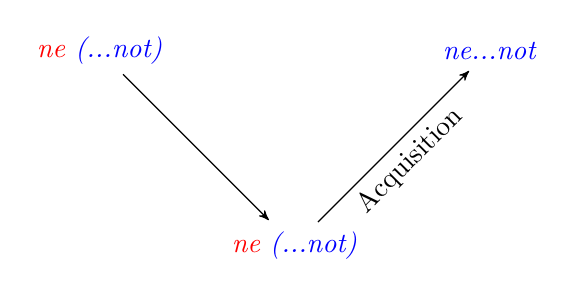
\begin{tikzpicture}[->,>=stealth',shorten >=1pt,auto,node distance=3.5cm]
      \node (C)  { \emph{\textcolor{red}{ne} \textcolor{blue}{(...not)}} };
      \node (D) [below right of=C] { \emph{\textcolor{red}{ne} \textcolor{blue}{(...not)}} };
      \node (E) [above right of=D] {\emph{\color{blue} ne...not} };
      \path[->] (C) edge node[sloped, anchor=center, below] {} (D)
      (D) edge node[sloped, anchor=center, below] {Acquisition} (E);
    \end{tikzpicture}
  \end{center}
	\caption{Syntactic acquisition as the cause of the first transition}
	\label{first-acquisition}
\end{figure}

So, the upper left \emph{\textcolor{red}{ne} \textcolor{blue}{(...not)}} indicates grammatical knowledge that includes both the pre-verbal and embracing form. But, there is no increase in the embracing form due to use. We indicate the increase in the embracing form due to acquisition as the upwards arrow in Figure \ref{first-acquisition}. The result of acquisition is that only the embracing form is acquired.  Again, while we only show a single step, this could just as well be the result of several iterations. Crucially, it is acquisition rather than use that is driving the increase in the embracing form. 

While we can present these two causes in isolation, another possibility is that both use and acquisition interact over time, giving rise to the embracing form. However, the important thing in any case is the form that an explanation must take. That is, for pragmatic use or syntactic acquisition to serve as explanations of the first transition we must demonstrate how they cause the increase in the frequency of the embracing form. We need a model of use or acquisition that makes both qualitative and quantitative predictions. That is, we need a model that predicts \emph{that} the first transition will happen, as well as \emph{how} it will happen.

The same requirements holds for the second transition.  We can represent what a pragmatic or syntactic explanation would like in Figures \ref{second-pragmatic} and \ref{second-acquisition}. For either to serve as an explanation, we would have to demonstrate how they cause the increase in \emph{\color{green} not} over time. Note that these requirements are independent of whether it makes sense to conceive of the second transition as a push-chain or whether we think that use or acquisition play any role whatsoever. In fact, it serves as an important check on any models we posit for the first transition. For example, if we have no reason to think that pragmatic use is what drives the second transition, then a model of the first transition based on use should not predict the second transition. 

\begin{figure}
  \begin{center}
    \begin{tikzpicture}[->,>=stealth',shorten >=1pt,auto,node distance=3.5cm]
      \node (C)  { \emph{\textcolor{blue}{(ne...)} \textcolor{green}{not}} };
      \node (D) [below right of=C] { \emph{\color{green} not} };
      \node (E) [above right of=D] {\emph{\color{green} not} };
      \path[->] (C) edge node[sloped, anchor=center, below] {Use} (D)
      (D) edge node[sloped, anchor=center, below] {} (E);
    \end{tikzpicture}
  \end{center}
	\caption{Pragmatic use as the cause of the second transition}
	\label{second-pragmatic}
\end{figure}


\begin{figure}
  \begin{center}
    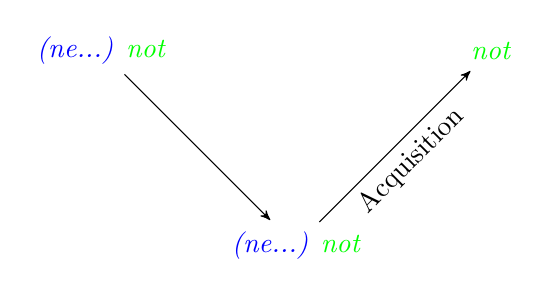
\begin{tikzpicture}[->,>=stealth',shorten >=1pt,auto,node distance=3.5cm]
      \node (C)  { \emph{\textcolor{blue}{(ne...)} \textcolor{green}{not}} };
      \node (D) [below right of=C] { \emph{\textcolor{blue}{(ne...)} \textcolor{green}{not}} };
      \node (E) [above right of=D] {\emph{\color{green} not} };
      \path[->] (C) edge node[sloped, anchor=center, below] {} (D)
      (D) edge node[sloped, anchor=center, below] {Acquisition} (E);
    \end{tikzpicture}
  \end{center}
	\caption{Syntactic acquisition as the cause of the second transition}
	\label{second-acquisition}
\end{figure}


\section*{Summary}

In this chapter we made the important terminological distinction between the formal and functional Jespersen cycles and noted the logical relationship between the two phenomena. An explanation of the formal cycle requires an explanation of the functional cycle, but not vice versa. importantly, given that the functional cycle can occur independently of the formal cycle, an explanation of the first may be fundamentally different from an explanation of the second. This guides our approach to explaining the two processes in the history of English, observed as the transitions from \emph{\textcolor{red}{ne}} to \emph{\color{blue} ne...not}  to \emph{\color{green} not}. 

In Part I we pursue an explanation of the functional cycle based on pragmatics. We present a mathematical framework for modeling how meaning is signaled in a population over time and apply it to modeling how pragmatic use leads to the transition from \emph{\textcolor{red}{ne}} to \emph{\color{blue} ne...not}, but not the transition from  \emph{\color{blue} ne...not}  to \emph{\color{green} not}. In Part II we turn to the formal cycle as a whole and evaluate whether a model of syntactic acquisition can explain either of the transitions, from \emph{\textcolor{red}{ne}} to \emph{\color{blue} ne...not} and from \emph{\color{blue} ne...not}  to \emph{\color{green} not}.



%%%%%%%%%
\part{The Functional Cycle}
% Evolutionary Game Theory
\chapter{Evolutionary Game Theory}
\label{evolutionary-game-theory}

\setlength{\epigraphwidth}{.9\textwidth}
\epigraph{We repeat most emphatically that our theory is thoroughly static. A dynamic theory would unquestionably be more complete and preferable.\\ --\citet[44-45]{von-neumann-morgenstern1944}\\ \hspace{12pt}

We shall now take up the ``mass-action'' interpretation of equilibrium points...It is unnecessary to assume that the participants have full knowledge of the total structure of the game, or the ability and inclination to go through any complex reasoning process.\\
--\citet[21]{nash1950}
%There are many situations, however, in which an individual is, in effect, competing not against an individual opponent but against the population as a whole.\\ --\citet[23]{maynard-smith1982}
}

Game theory is a branch of applied mathematics originally developed by \cite{von-neumann-morgenstern1944} that models human decision-making when the actions, outcomes, and preferences of multiple agents are intertwined. This differs from decision theory, where a single agent is faced with a choice to bring about his or her most preferred outcome. Rather, a game arises when the choices made by each player crucially depend on those made by others. It is this interdependence that distinguishes game theory and makes it such a useful tool in understanding social interactions, from the routes we choose to drive to work to the way we use words to mean things.

While 



The rest of this chapter provides an outline of the crucial concepts for our application of evolutionary game theory to language change. First, we offer a general overview of the dimensions along which games vary. We focus on two simple games, and develop intuitions about expected behavior. Second, we define a set of solution concepts that can be applied to predict behavior in the two simple games. We discuss the limitations of solutions concepts for predicting behavior. Third, we supply game dynamics and examine the trajectory of the population under those game dynamics for the two simple games. We then we define signaling games as a natural model of communication and present the simplest case. Finally, we present a generalized means of describing the dynamics of arbitrarily complex signaling games.


Taking up one aspect of this first example, we will assume that the vast majority of people would prefer to avoid car accidents. When driving a car, this is straightforwardly achievable by always being on the opposite side of the road of the next oncoming vehicle. We can think about this from the perspective of two drivers approaching each other. Each driver has the choice of driving on the left or the right. Both parties would prefer to coordinate on driving on whichever side. The side of the road that best achieves the outcome of not crashing is irrelevant, but it depends on how both parties drive. If both parties choose to drive on the right, from their own perspective, then they will avoid each other. Likewise if they choose to drive on the left.

The solutions to this interaction are readily apparent, everyone should choose one side of the road or the other. Provided that both drivers choose the same side, then neither has an incentive to switch. This fundamental insight into behavior in games is what defines a \emph{Nash equilibrium}: the action of all agents is optimal given the choices of all other agents. Yet, grounding this solution in rationalistic terms requires a little more effort. First, it requires that all agents are \emph{rational}, acting to maximize their own benefit. This is implicit in our example above, most humans prefer to avoid being injured. Second, it requires that players have \emph{common knowledge} of the game structure, including the actions available to all players, the outcomes of different combinations, and know that they all know these things, and so forth. At least for this game it follows naturally from the number of sides of the road there are, and the ability to reason about collisions, but it is not always so straightforward. Finally, it requires that agents have \emph{equilibrium knowledge}, that they are able to accurately anticipate the actions of other players.  This last requirement may seem readily apparent, at least for the example of driving, but it deserves further comment. 

Depending on the country, we know that everyone will drive on one side of the road. In fact, there are laws and legal repercussion for not doing so. Yet, if we abstract away from our everyday experience in this particular case, the problem becomes clearer. For example, imagine that you are asked to choose between two options, that another person has been asked to choose between the same two options, that both of you have received the same instructions, and that you will both succeed if you choose the same option. These starker terms may seem to border on the absurd, but they bring the problem into relief. Their absurdity lies in the fact that it does not do to reason about \emph{this} option or \emph{that} option, because there is nothing to distinguish the two. There is no \emph{thisness} or \emph{thatness} to motivate one choice or the other. That is, there is no rule of the road that simply states "Drive on the right". Instead, we are faced with the problem of deciding the undecidable, as Aristotle, a bit sarcastically put it in his \emph{On the Heavens}:
%Buridanian 

\begin{quotation}
%men who, though exceedingly hungry and thirsty, and both equally, yet being equidistant from food and drink, is therefore bound to stay where he is-even so
[A] man, being just as hungry as thirsty, and placed in between food and drink, must necessarily remain where he is and starve to death.
\end{quotation}

We are particularly good at looking for reasons why one option is preferable, or more likely to be chosen than another. For example, if we were to enrich our description above to a choice between an option \emph{A} or an option \emph{B}, an intuitive rationale would be to choose \emph{A}. The reason for doing so being that \emph{A} comes first in the alphabet, and that both people might expect each other to know this. There is some intuitive \emph{thisness} about option \emph{A} that we can leverage on the assumption that it will be readily apparent to others as well.  \citet[57]{schelling:1960} called these partial escapes from the dilemma of equilibrium knowledge \emph{focal points} ``for each person�s expectation of what the other expects him to expect to be expected to do." In the pre-cellular age, Schelling posed the following scenario: ``Tomorrow you have to meet a stranger in NYC. Where and when do you meet them?" The intuitive meeting place of Schelling's day was Grand Sentral station at noon. The rationale for both choices is that they are prominent in their respective geographical and temporal landscapes. Experimental results demonstrate that people are generally quite  good at grounding their coordination via reasoning about these kinds of focal points \citep{mehta-etal1994,mehta-etal1994b,bardsley-etal2010}. 


But, even with our ability to reason about what we might expect others to expect us to expect them to expect us to do, we still cannot perfectly anticipate what others will do. That is, focal points are useful heuristics, but they are never foolproof: not everyone would choose option \emph{A} or grand central station at noon. In fact, it would not be foolish for example to suggest meeting at Times Square at noon. The problem of justifying equilibrium in general still remains. Nash himself was well aware of this problem, which was in part what prompted his consideration of a ``mass-action'' interpretation of equilibria.\footnote{The main motivation was understanding \emph{mixed Nash equilibria}, which involve some probability distribution over actions. \cite{nash1950,nash:1950,nash:1951} proved that such an equilibrium is guaranteed to exist. What it means for an individual to adopt the corresponding \emph{mixed strategy} is not unproblematic. For a discussion of these problems see \cite{aumann1985}, and for the population approach see \cite{rosenthal1979}.} In short, this change in perspective moves from focusing on a single agent to a population of agents that need not have either common knowledge or equilibrium knowledge.  This perspective was naturally taken up in applications of game theory to biology, where loosening some of the equilibrium requirements was both reasonable and necessary \citep{maynard-smith1982}. This move also came with the reinterpretation of the game-theoretic machinery: actions were not choices to be made by the individual, but genetically pre-determined responses; the utility derived from a particular outcome was not a numerical representation of preferences, but a measure of Darwinian \emph{reproductive fitness}. 

This turn towards the biological allowed for further developments towards the explicitly dynamic theories that \cite{von-neumann-morgenstern1944} envisioned.  Drawing on the mechanics of population genetics, \cite{taylor-jonker:1978} offered the first \emph{evolutionary game dynamics}, christened the \emph{replicator dynamics} by  \cite{eigen-schuster1979}, which explicitly defined how a population changes over time due to biological reproduction.  This new approach allowed for insights into not just whether a population would remain at some equilibrium state if it started there, but also if the population would reach that equilibrium state in the first place. While successively detailed refinements of Nash equilibria were proposed with more and more unrealistic assumptions, evolutionary game theory offered a means of understanding equilibrium behavior under much simpler assumptions. 

Despite its biological roots, however, work in evolutionary game theory has discovered profound connections with the rationalistic approach to equilibrium behavior. That is, the equilibrium predictions of the rationalistic approach often correspond to the effect of natural selection captured by evolutionary game dynamics. Perhaps more surprisingly, some of these game dynamics can be derived not just from the mechanics of biological reproduction, but from particular kinds of decision making or behavior. For example, the replicator dynamics defined by \cite{taylor-jonker:1978} can also be derived from particular forms of imitation \citep{schlag1998,bjornerstedt-weibull1996} and learning \citep{borgers-sarin1997}. The fact that such  diverse foundations yield the same dynamics is both surprising and compelling. More importantly, these commonalities show that if we interpret \emph{evolution} in this broader sense that includes both biological and social change, then evolutionary game theory can serve as a powerful tool.

The rest of this chapter provides an outline of the crucial concepts for our application of evolutionary game theory to language change. First, we offer a general overview of the dimensions along which games vary. We focus on two simple games, and develop intuitions about expected behavior. Second, we define a set of solution concepts that can be applied to predict behavior in the two simple games. We discuss the limitations of solutions concepts for predicting behavior. Third, we supply game dynamics and examine the trajectory of the population under those game dynamics for the two simple games. We then we define signaling games as a natural model of communication and present the simplest case. Finally, we present a generalized means of describing the dynamics of arbitrarily complex signaling games.


\section{Games}
\label{Games}

There are several major dimensions along which games can vary.\footnote{See \cite{dixit-skeath2004} for a gentle introduction to game theory, \cite{tadelis2013} for a thorough but balanced introduction, and \cite{osborne-rubinstein1994} and \cite{fudenberg-tirole1991} for more advanced mathematical treatments.} Here we focus on several dimensions that are relevant for the case of communication and thus language change.  The first dimension we will consider is the order which players make their decisions. If all players make a decision at the same time, then the game is a \emph{simultaneous} game. If players make their decisions in a particular order, then the game is a \emph{sequential} game. Communication is sequential insofar as we separate out the transmission and interpretation of a signal. Thus, we will be concerned with sequential games.

The second dimension along which games vary is whether or not players have private information that affects others' payoffs. If players do have private information then the game is one \emph{incomplete information}, otherwise it is one of \emph{complete information}. Intuitively, this is the crucial aspect of communication. Speakers have some private information  that hearers do not. We cannot read minds, thus we have to communicate. This asymmetry of information is crucially tied to the third dimension along which games vary. Namely, if the set of actions available to the different players differs or if the payoff from the same action differs, then the game is considered \emph{asymmetric}. If the actions are identical for all players and if the outcome of actions are independent of who takes them then the game is \emph{symmetric}. There are clearly two distinct roles in the act of communication, thus we will be concerned with asymmetric sequential games of incomplete information.

In this section we introduce to simple simultaneous games of complete information.  We develop the intuitions required for the application of equilibrium concepts and dynamic analysis before moving on to the more complicated asymmetric sequential games of incomplete information known as \emph{signaling games} that will be used in subsequent analysis. 

%
%The final dimension along which games vary is whether the players have the same or similar preferences over outcomes. 
%
%The space of possibilities is fairly large, but there are indeed several broad distinctions between classes of games.



%If they do, then we call the game one of \emph{common interests}. If they do not, then we call the game one of \emph{conflicting interests}. A special case of conflicting interests is where players have perfectly opposing interests, a gain for one player is an equal and opposite loss for the other. These kinds of games are \emph{constant} or \emph{zero-sum games}.

%We vary whether the games are constant-sum or not, and hence games of common or conflicting interests as well as symmetric versus asymmetric.

%Interestingly, there are some logical relationships between these dimensions. For example, a game of incomplete information is necessarily asymmetric. Likewise, a constant-sum game is also asymmetric. 

The first simple example we consider is parallel to the case of choosing which side of the road to drive on, and is often referred to as a \emph{coordination game}. There are two players who we will refer to as \emph{Row} and \emph{Column}, for reasons that will become clear later on. Each player has a choice between two options, \emph{A} and \emph{B}. We we will refer to these options as \emph{pure strategies}.\footnote{This is in contrast to \emph{mixed} strategies, which specifiy a probability distribution over pure sender strategies, $\sigma = p_1 s_1 + ... + p_k s_k$, where $\sum_i p_i = 1$.}  That is, the set of pure strategies available to \emph{Row} is $S_R = \{A, B \}$, and the set of actions available to \emph{Column} is $S_C = \{A, B \}$. The set of all combinations of \emph{Row} and \emph{Column} strategies constitute the \emph{strategy profiles} of the game. That is, for each $s_i \in S_R$ and $s_j \in S_C$, the tuple $\langle s_i, s_j \rangle$ constitutes a strategy profile. 

Now, we can capture the intuition that both players prefer to avoid crashing by defining utility functions over outcomes for both players. \emph{Row}'s utility function is a function from strategy profiles to real numbers $U_R : \langle s_i, s_j \rangle \rightarrow \mathbb{R}$. Likewise \emph{Column}'s utility function is a function from strategy profiles to real numbers $U_C : \langle s_j, s_i \rangle \rightarrow \mathbb{R}$. In fact, we can drop the subscripts entirely, if we define the two utility functions in the following way.

\begin{equation}
U(s_i, s_j) = U_{R}(s_i, s_j) =  U_{C}(s_j, s_i) =
\left\{
	\begin{array}{ll}
		1  & \mbox{if } s_i = s_j \\
		0 & \mbox{else}
	\end{array}
\right.
\end{equation}
Note that utilities are only important insofar as they represent an ordinal ranking over outcomes. In other words, there is nothing particularly special about $0$ and $1$ as opposed to say $3.277$ and $110$ other than the fact that in both cases the first is less than the second. However, there is something important about the fact that $U(A, A) = U(B, B)$. This simply reflects the fact that either rule of the road is equally useful for avoiding collisions.

With these utility functions defined, we can present the game in a slightly more compact \emph{normal form} as in Table \ref{CG}. The strategies for \emph{Row} and \emph{Column} are listed to the left and above respectively, hence the names. By convention, for each cell of Table \ref{CG}, the payoff for \emph{Row} is listed first, followed by the payoff for \emph{Column}. The reason why coordination games are symmetric is that both $U_R$ and $U_C$ define symmetric matrices. Intuitively, we could rotate Table \ref{CG} around its diagonal and nothing would change;  the payoffs for one player are the transpose of the other. In fact, we could represent the payoffs in this symmetric game as a matrix that captures this symmetry.

\begin{table}\centering
\begin{tabular}{lll}
\hline\noalign{\smallskip}
 & A & B \\
\noalign{\smallskip}\hline\noalign{\smallskip}
A & $1, 1$ & $0, 0$ \\
B & $0, 0$ & $1, 1$ \\
\noalign{\smallskip}\hline
\end{tabular}
\caption{Coordination Game}
\label{CG}
\end{table}


\begin{equation}
U(s_i, s_j) = 
 \begin{pmatrix}
 1 & 0\\
 0 & 1\\
 \end{pmatrix}
\end{equation}


With these definitions in place, we return to the reasoning above. Namely, both players want to coordinate on playing either $A$ or $B$. If one player chooses $A$, then the other should as well. If one player chooses $B$, then the other should as well. But, there is no guarantee that the other player will choose $A$ or $B$. Again, simply knowing that both would be good outcomes does not guarantee that both players will choose one or the other.

We can modify the game in a simple but substantial way by altering the payoff structure. That is, imagine the case where the utility functions of the sender and receiver are defined as the following.

\begin{equation}
 U_{R}(s_i, s_j) =
\left\{
	\begin{array}{ll}
		1  & \mbox{if } s_i \neq s_j \\
		0 & \mbox{else}
	\end{array}
\right.
\end{equation}

\begin{equation}
 U_{C}(s_j, s_i) =
\left\{
	\begin{array}{ll}
		1  & \mbox{if } s_i = s_j \\
		0 & \mbox{else}
	\end{array}
\right.
\end{equation}
That is, the payoffs of \emph{Row} are diametrically opposed to that of \emph{Column}. This game, called \emph{matching pennies} has the following simple rules. Both players choose between heads $H$ or tails $T$. One player wins if the coins match, and the other player wins if the coins do not match. The resulting game is summarized in Table \ref{MP}. Matching pennies is a constant-sum asymmetric game, the components of every cell in Table \ref{MP} sum to a constant. Except in the trivial case where all outcomes yield the same utility for both players, constant-sum games are asymmetric. That is, we cannot represent the payoffs as a single value without losing crucial information.  


\begin{table}\centering
\begin{tabular}{lll}
\hline\noalign{\smallskip}
 & H & T \\
\noalign{\smallskip}\hline\noalign{\smallskip}
H & $0, 1$ & $1, 0$ \\
T & $1, 0$ & $0, 1$ \\
\noalign{\smallskip}\hline
\end{tabular}
\caption{Matching Pennies}
\label{MP}
\end{table}
 Unlike the coordination game, players want to anti-coordinate with each other.  That is, if \emph{Row} plays $H$, then \emph{Column} would prefer to play $H$, but if \emph{Column} plays $H$ then \emph{Row} would prefer to play $T$. This poses another interesting problem. If both players have opposing interests, how should they act? It is clearly not feasible to pick one strategy or the other, as this would leave either player open to exploitation by the other. It would seem then that the best both players can do is to flip a coin and play whichever side comes up.

Before turning to defining equilibria, we need to note one last aspect of utility. As a case in point, let us assume that when playing matching pennies as \emph{Row}, we know that our opponent has a certain probability of playing $H$, and thus a certain probability of playing $T$. Let $p$ be the probability that our opponent plays $H$. Given that we are never certain of which strategy our opponent will play, we want to know the \emph{expected utility} of choosing one strategy or another. With slight abuse of notation, this is just the following.\footnote{This is just the expected value of a random variable. To take a simple example, imagine if we flipped a fair coin, counting heads as a $1$ and tails as a $0$, then the expected value of the coin flip would be $\frac{1}{2}$}

\begin{equation}
	E[U_R(H)] = pU_R(H,H) + (1-p)U_R(H,T) = (1-p)
\end{equation}
Expected utility is crucial in determining behavior in cases where there is uncertainty due to probabilistic behavior.

\section{Equilibria}

A game by itself does not constitute a model in the technical sense. It is a mathematical structure that describes the players preferences and strategies, but it does not predict their behavior. To do so it must be supplemented with a \emph{solution concept} that predicts the conditions under which particular outcomes will obtain. Here we define two related solution concepts, note how they apply to the simple games we defined above, and note their limitations for predicting behavior.

\subsection{Nash Equilbria}

Perhaps the most widely used solution concept is that of a \emph{Nash equilibrium}, which specifies when players have an incentive to unilaterally deviate from a given strategy profile. We provide a definition and apply the concept to our simple games.

For a given strategy profile where $s_i$ is the strategy of a particular player, let $s_{-i}$ be the set of strategies for all other players. We have the following definition.

\begin{definition}
 A strategy profile $\langle s_i^*, s_{-i}^*\rangle$ is a \emph{Nash equilibrium}
if and only if:
  \begin{itemize}
   \item $\forall i$, $\forall s_i \in S_i$, such that $s_i \neq s_i^*$, $E[U(s_i^*,s_{-i}^*)] \geq
E[U(s_i,s_{-i}^*)]$
  \end{itemize}
\end{definition}


%\begin{definition}
% A strategy profile $\langle s^*, r^*\rangle$ is a \emph{Nash equilibrium}
%if and only if:
%  \begin{itemize}
%   \item For all $s \in S$, such that $s \neq s^*$, $E[U_S(s^*,r^*)] \geq
%E[U_S(s,r^*)]$
%  \item For all $r \in R$, such that $r \neq r^*$, $E[U_R(s^*,r^*)] \geq
%E[U_S(s^*,r)]$
%  \end{itemize}
%\end{definition}

This simply states that no players can do better by individually changing his or her strategy from the equilibrium profile.  No one has an incentive to change, so everyone keeps doing what they are doing, hence the term equilibrium.  That is, every player's current strategy is a \emph{best response} to everyone else's. Note that this best response need not be unique to constitute an equilibrium. This follows from the fact that the inequalities in the definition are not strict. We can, however, impose uniqueness in these best responses by requiring that the inequalities in the definition be strict. A \emph{strict Nash equilibrium} results, meaning that players can only ever do worse if they unilaterally deviate from the equilibrium. 


%Strict Nash equilibria are thus a proper subset of Nash equilibria. 

%Since we are interested not just in the behavior of two individuals, but rather the aggregate behavior of a population, we want a broader notion of equilibrium. In particular, we might ask whether a given population is susceptible to change.

%The two conditions simply state that neither the sender nor the receiver can do better by individually changing his or her strategy from the equilibrium profile.  The sender's strategy is his \emph{best response} to the receiver's strategy, and the receiver's strategy is likewise her best response to the sender's strategy. Note that these best responses need not be unique to consitute an equilibrium. This follows from the fact that the inequalities in the definiton are not strict. We can, however, impose uniqueness in these best responses by requiring that the inequalities in the definition be strict. A \emph{strict Nash equilibrium} results, meaning that players can only ever do worse if they unilaterally deviate from the equilibrium. Strict Nash equilibria are thus a proper subset of Nash equilibria.

We can now apply this solution concept to the games we described above. First, we look at the coordination game. We already noted that coordinating on one strategy or the other seems to be an intuitive solution. The conditions for $\langle A, A \rangle$ and $\langle B, B \rangle$ to be Nash equilibrium are the following.

\begin{equation}
		E[U(A, A)] \geq E[U(B, A)]
\end{equation}

\begin{equation}
		E[U(B, B)] \geq E[U(A, B)]
\end{equation}
In fact, looking at the payoffs in Table \ref{CG}, both of these outcomes meet the definition of a strict Nash equilibrium. Both players can only do \emph{worse} by deviating from the equilibrium.

There is one last kind of equilibrium to consider. Imagine that both players choose $A$ with probability $p$ and $B$ with probability $(1-p)$. The expected utility for both pure strategies are the following.

\begin{equation}
	E[U(A)] = pU(A,A) + (1-p)U(A,B) = p
\end{equation}	

\begin{equation}
	E[U(B)] = pU(B,A) + (1-p)U(B,B) = (1 - p)
\end{equation}	
Note that these are equal to each other when $p=\frac{1}{2}$. Now suppose that an agent plays a mixed strategy $\sigma$ that strikes this balance by playing each strategy half of the time. We can show that this mixed strategy is a Nash equilibrium by comparing how another mixed strategy would fare against it. First, note that the expected utility of $\sigma$ against itself is $\frac{1}{2}$.

\begin{equation}
	\begin{split}
		E[U(\sigma, \sigma)] &= \frac{1}{2} \cdot \frac{1}{2}U(A,A) + \frac{1}{2} \cdot \frac{1}{2}U(A,B) + \frac{1}{2} \cdot \frac{1}{2}U(B,A) + \frac{1}{2} \cdot \frac{1}{2}U(B,B) \\
		&= \frac{1}{2}
	\end{split}
\end{equation}
Second, consider the expected utility of any alternate strategy $\sigma'$ that plays $A$ with probability $p$ and $B$ with probability $(1-p)$. Note that this includes the pure strategies as extremes, $A$ where $p=1$ and $B$ where $p=0$.

\begin{equation}
	\begin{split}
		E[U(\sigma', \sigma)] &= \frac{1}{2} \cdot pU(A,A)  + \frac{1}{2} \cdot pU(A,B) + \frac{1}{2} \cdot (1-p)U(B,A)\\ &+ \frac{1}{2} \cdot (1-p)U(B,B) \\
		&= \frac{1}{2}
	\end{split}
\end{equation}
That is, if the other player plays according to strategy $\sigma$, then no matter what the other does, they will receive a fixed expected utility. This means that if the other player plays each option evenly, there is nothing to be gained from switching from the same strategy. That is, any mixed strategy will do just as well.

\begin{equation}
	E[U_R(\sigma, \sigma)] \geq E[U_R(\sigma', \sigma)]
\end{equation}
Thus, there are two pure Nash equilbria and one mixed Nash equilibria in this coordination game. This mixed Nash equilibrium is the unsatisfying solution mocked by Aristotle above. That is, by committing to neither, both players are worse off; each player receives an expected utility of $\frac{1}{2}$ compared to the expected utility of $1$ at the pure strategy equilibria. But intuitively, this indecision is precarious, any slight reason to choose one or the other would suffice to break the symmetry and motivate one solution or the other. We find that  this intuition is indeed the case when we turn to dynamics below.

In contrast to the coordination game, there are no pure strategy equilibrium for matching pennies. For any pure strategy profile, one of the players will have an incentive to change her strategy: for $\langle A, A \rangle$ and $\langle B, B \rangle$, \emph{Row} will have an incentive to deviate; $\langle A, B \rangle$ and $\langle B, A \rangle$, \emph{Column} will have an incentive to deviate. In fact the mixed strategy where both players split the difference between heads and tails is the unique Nash equilibrium. To see this note that the mixed strategy yields an expected utility of $\frac{1}{2}$ and that any alternate mixed strategy also yields an expected utility of $\frac{1}{2}$. Note that since any mixed strategy yields the same payoff against the mixed strategy, then it is not 
strict.

\subsection{Evolutionarily Stable Strategies}

%Since we are interested not just in the behavior of a given sender and receiver, but rather the aggregate behavior of a population, we want a broader notion of equilibrium. In particular, we might ask whether a given population is susceptible to change. When considering \emph{asymmetric games}, such as signaling games, where players have different roles, we are actually concerned with two populations: a sender population and a receiver population. To determine the stability of the two populations we can consider a \emph{symmetrized} version of the signaling game, where individuals act as both sender and receiver. A strategy in the symmetrized game is thus a strategy profile of the asymmetric game.

While the concept of a Nash equilibrium is particularly useful, we we are interested not just in the behavior of two individuals, but rather the aggregate behavior of a population. Thus, we might want a broader notion of equilibrium. In particular, we might ask whether an entire population is susceptible to change, rather than the behavior of two individuals.  We define a criterion that captures this level of description, note its limitations, and apply it to our simple games.

At the population level, the most relevant concept is that of an \emph{evolutionarily stable strategy} \citep{maynard-smith-price:1973,maynard-smith1982}. In a symmetric game where $U(s^*, s)$ is the payoff to an agent using strategy $s^*$ against an agent using strategy $s$, we have the following definition.

\begin{definition}
 A strategy $s^*$ is an evolutionarily stable strategy (ESS) if and only if, for all alternate strategies $s$:
\begin{itemize}
 \item $U(s^*, s^*) \geq U(s,s^*)$
 \item If $U(s^*, s^*) = U(s,s^*)$ then $U(s^*, s) > U(s,s)$
\end{itemize}
\end{definition}

Note that the first condition is the same as that of a Nash equilibrium.  The second condition limits evolutionarily stable strategies to a proper subset of Nash equilibria. A straightforward interpretation of this definition can be had by imagining a population composed entirely of individuals playing $s^*$. Suppose some small proportion, $1 \gg \epsilon > 0$, of individuals playing the alternative $s$ is introduced into the population. The following inequality holds if and only if $s^*$ is an ESS.

\begin{equation}
\label{ESSlinear}
(1-\epsilon )U(s^*,s^*) + \epsilon U(s^*,s)  > (1-\epsilon)U(s,s^*) + \epsilon U(s,s)
\end{equation}
For any sufficiently small influx of the alternate strategy, the expected payoff of the incumbent strategy in the resulting population is strictly greater than that of the alternate. Intuitively, $s^*$ is stable because selection will carry the population back to playing $s^*$. Loosely speaking, a strategy is evolutionarily stable if it is resistant to invasion by alternate strategies. That is, when an entire population plays the incumbent strategy the incumbents do at least as well as an alternate. If the alternate does as well, then the incumbent strategy should do better than an alternate in an all-alternate population.

While evolutionarily stable strategies are a useful refinement of Nash equilibria, they only offer particular kinds of insight. That is, under the standard \emph{equilibrium methodology}  \citep{huttegger-zollman2013}, the state of a population is often justified by some special status. For example, the persistence of particular states of the population is due to it being an evolutionarily stable strategy. However, this kind of explanation looses some of its explanatory bite if there either multiple evolutionarily stable strategies, or none. If we apply the solution concept to the games we described above, these problems becomes clear. First, we look at the coordination game. We can use the reformulation of the criterion above to give the conditions for $\langle A, A \rangle$ and  $\langle B, B \rangle$ to be evolutionarily stable strategies. 

\begin{equation}
		(1 - \epsilon)U(A,A) + \epsilon U(A,B) > (1-\epsilon)U(B,A) + \epsilon U(B,B)\
\end{equation}

\begin{equation}
		(1 - \epsilon)U(B,B) + \epsilon U(B,A) > (1-\epsilon)U(A,B) + \epsilon U(A,A)\
\end{equation}
That is both of the pure strategy Nash equilibria for the coordination game are evolutionarily stable strategies if $\frac{1}{2} > \epsilon$. Assuming that $1 \gg \epsilon > 0$, this is guaranteed,  but this condition also has another interpretation. That is, $\frac{1}{2} > \epsilon$ defines the \emph{invasion barrier}, the influx required to move the population from one equilibrium to the other. This makes intuitive sense, if the population of the United States moved to the United Kingdom, and insisted on maintaining the same traffic patterns, then everyone would best be served by adopting the majority pattern.

We can also consider the condition for the mixed Nash equilibrium to be  an evolutionarily stable strategy.

\begin{equation}
		(1 - \epsilon)U(\sigma,\sigma) + \epsilon U(\sigma,A) > (1-\epsilon)U(A,\sigma) + \epsilon U(A,A)\
\end{equation}
Remembering from above that the expected utility of the mixed strategy against itself and any strategy against the mixed strategy are both $\frac{1}{2}$, we know that the mixed strategy state is not evolutionarily stable. Note that the conditions for $B$ to invade the mixed state are the same as for $A$. The invariability of the mixed strategy state validates our intuitions about its instability.

Turning to asymmetric games, such as matching pennies, where players have different roles, we are actually concerned with two populations. To determine the stability of the two populations we can consider a \emph{symmetrized} version of the game, where individuals have strategies for both roles. A strategy in the symmetrized game is thus a strategy profile of the asymmetric game. In the case of symmetrized asymmetric games, the criterion for stability is actually simpler. A strategy profile is evolutionarily stable if and only if it constitutes a strict Nash equilibrium in the original asymmetric game \citep{selten:1980}. This means that the mixed strategy in matching pennies is not an evolutionarily stable strategy, the game simply does not have one. Thus, the justification of a particular state of the population as an evolutionarily stable strategy is off the table.

\citet[8]{maynard-smith1982} noted both of these problematic conditions, but considered them to be ultimately unproblematic insofar as they are obvious exceptions. However, the obviousness of exceptions becomes less clear as games become more complex. \cite{huttegger-zollman2013} provide a compelling example of where intuitions fail and focusing on equilibria is particularly misleading. The solution to these limitations is to use both static equilibrium concepts along with an explicitly dynamic perspective.




%It is important to note, despite the dynamic terminology, an ESS is still an essentially static concept.  

%But, we have not been explicit about the game dynamic that does the carrying. \cite{taylor-jonker:1978} introduced the replicator dynamic to explicitly address the dynamical aspects of evolutionarily stable strategies. Thus there is a fundamental connection between the two. 

%We may naturally expect some form of selection to eliminate strategies with lower expected payoffs and carry the population back to playing $s^*$.

%This connection does not necessarily extend to other game dynamics though. 


%For the Lewisian signaling game described above, where states are equiprobable, $\delta(t_1) = \delta(t_2) = \frac{1}{2}$, the only strict equilibria are those where senders employ different signals for each state, and receivers map those messages to the appropriate actions. In other words, the senders \emph{separate} themselves and receivers respond accordingly. These equilibria are referred to as \emph{separating equilibria}. There are also equilibria where senders \emph{pool} themselves together and use only a single message. Receivers are indifferent between actions; they receive the same expected utility for taking either action. These are referred to as \emph{pooling equilibria}. Note that these pooling equilibria are not strict insofar as any action taken by the receiver yields the same expected utility. Thus, in the case of perfectly-aligned interests, separating equilibria are the only evolutionarily stable strategies.


\section{Dynamics}

While the term suggests a dynamic interpretation, equilibria, including evolutionarily stable strategies, are static solution concepts. They tell us whether a strategy is resistant to invasion or innovation, but tell us nothing about how the population got there in the first place, or where it might go next. To understand how a population changes over time, a particular set of \emph{game dynamics} must be supplied.\footnote{See \cite{mcelreath-boyd2008} for a general introduction to the mathematical modeling of social evolution, \cite{gintis2000} for a comprehensive introduction to evolutionary game theory, and \cite{weibull1997} and \cite{hofbauer-sigmund:1998} for more advanced mathematical treatments. For a general introduction to non-linear dynamical systems see \cite{strogatz2014} and \cite{hirsch-smale1974} for a more mathematical treatment. See \cite{sandholm2010} for a thorough and insightful grounding of evolutionary game dynamics in individual behavior.}  These provide a  description for how a population, or populations, changes from one point in time to the next.

%\begin{itemize}
%	\item Behaviors that have been successful are reinforced, and those that have been unsuccessful are repressed. In the continuous time limit where the change in x and y on any given time step goes to zero under some plausible assumptions, it is possible to show (11) that reinforcement learning dynamics are described by the coupled replicator equations (see Notes) of the form
%\end{itemize}

In what follows we will focus on the replicator dynamics. The reasons for doing so are twofold. First, they are the most extensively studied dynamics and share a number of mathematical properties with a larger set of game dynamics \citep{hofbauer-sigmund:1998}.  This makes establishing results and connecting them to a broader class of dynamics more straightforward. They have also found broad application in modeling economic \citep{samuelson:1997, cressman:2003} and social behavior \citep{skyrms:1996,skyrms:2004,skyrms:2010}. Second, they have a natural interoperation as particular form of learning \citep{borgers-sarin1997,fudenberg-levine:1998}, which we will return to later on. We begin by defining the form of the replicator dynamics for symmetric and asymmetric games. We then outline general methods for assessing the stability of particular states. With these definitions and methods in place, we return to our simple games from  above.

The intuition behind the replicator dynamics is that  more successful strategies increase in frequency. In particular, strategies that are more successful than the population average increase in share of the population. For the case of a symmetric game, let $\mathbf{x}$ be a vector that represents the composition of the population, where $x_i$ represents the proportion of $s_i$, and the utility function is represented by the matrix $\mathbf{A}$. The change of $x_i$ in the population can be given as the following.

\begin{equation}
	\mathbf{\dot{x}}_i = \mathbf{x}_i((\mathbf{Ax})_i - \mathbf{x^{T}Ax})
\end{equation}
We begin by interpreting the second part of the equation. The first portion simply provides the expected utility of $s_i$ given the current composition of the population. The second portion simply provides the average expected utility given the current composition of the population. The difference between these two is how much better a strategy $s_i$ does than the average. If $s_i$ does better than the average, then its share of the population will increase; if $s_i$ does worse than the average, then its share will decrease. This increase or decreases is weighted by the current proportion of strategy in the population.

As a simple case in point, let us return to the coordination game from above. To start, let $p$ be the proportion of the population playing $A$. Then the population vector is given by the following.

\begin{equation}
\mathbf{x} = \begin{pmatrix} x_A\\ x_B \end{pmatrix}
\end{equation}
The payoff matrix, is given by the following.
\begin{equation}
\mathbf{A} = \begin{pmatrix} 1 & 0\\ 0 & 1 \end{pmatrix}
\end{equation}

Since there are only two strategies in the symmetric game, we only need to keep track of the proportion playing one, $x_A = 1 - x_B$. For simplicity, we will keep track of the proportion playing $A$, so we can drop the subscript, and note that it evolves according to the following replicator dynamic.
\begin{equation}
	\dot{x} = x(1 - x)(2x - 1)
\end{equation}
The \emph{rest points} of the replicator dynamic for the coordination game are the points where this equation is equal to zero. That is, they are the points where the motion of the system is at rest. The rest points of the dynamic are exactly the states that correspond to Nash equilibria. Namely, when $x = 0, 1, \frac{1}{2}$. 

%Note that this holds by definition. That is, strategies are invariant when they do as well as the average payoff.

% where $f_i(\mathbf{y})$ is the expected utility of $s_i$ given the receiver population, and the average sender expected utility is given as $f(\mathbf{y}) = \sum_{i} x_if_i(\mathbf{y})$.
We can define the parallel case for asymmetric games, where there are two populations denoted by  $\mathbf{x}$ and $\mathbf{y}$, along with two payoff matrices $\mathbf{A}$ and $\mathbf{B}$

\begin{equation}
	\mathbf{\dot{x}}_i = \mathbf{x}_i((\mathbf{Ay})_i - \mathbf{x^{T}Ay})
\end{equation}

\begin{equation}
	\mathbf{\dot{y}}_i = \mathbf{y}_i((\mathbf{Bx})_i - \mathbf{y^{T}Bx})
\end{equation}
For matching pennies, we define the following components.

\begin{equation}
\mathbf{x} = \begin{pmatrix} x_H\\ x_T \end{pmatrix} \hspace{12pt} \mathbf{y} = \begin{pmatrix} y_H\\ y_T \end{pmatrix}
\end{equation}
The payoff matrix, is given by the following.
\begin{equation}
\mathbf{A} = \begin{pmatrix} 0 & 1\\ 1 & 0 \end{pmatrix} \hspace{12pt} \mathbf{B} = \begin{pmatrix} 1 & 0\\ 0 & 1 \end{pmatrix}
\end{equation}
Again, simplifying our notation by omitting subscripts, these yield the following coupled replicator dynamics.

\begin{equation}
	\begin{split}
	\dot{x} &= x(1-x)(1-2y)\\
	\dot{y} &= y(1-y)(2x-1)
	\end{split}
\end{equation}
Note that the rest points of the replicator dynamics for matching pennies include more than the single Nash equilibrium we noted. That is, the point $(x,y) = (1,1)$ where both populations only play heads is a rest point of the dynamics. However, this is certainly not an outcome we would expect. Thus, we need more information than just the rest points.  We are, however, interested in the relation between the entire state space and these rest points. In particular, we are interested in whether the populations will move towards or away from particular states. That is, we want to know about the stability of the rest points.

A bit more formally, for a state space $\mathbf{x} = \{x_1, x_2,...,x_n \}$, a solution trajectory through the state space over time $\mathbf{x(t)}$ is governed by the differential equations defined by the game dynamics $\mathbf{\dot{x}} = \{\dot{x}_1, \dot{x}_2,...,\dot{x}_n \}$. The rest points of the system are states where the differential equations vanish; any trajectory starting at a rest point will remain there at rest. For a rest point $\mathbf{x^*}$, if $\mathbf{x(0)} = \mathbf{x^*}$ then $\mathbf{x(t)} = \mathbf{x^*}$ for all times $t > 0$, since $\mathbf{\dot{x}} = 0$.  The criteria we listed above, then, require the following definition.

\begin{definition}
 A rest point $\mathbf{x^*}$ is asymptotically stable if and only if:
\begin{enumerate}
     \item For every neighborhood $V$ of $\mathbf{x^*}$, there is a neighborhood $V'$ of $\mathbf{x^*}$ such that if $\mathbf{x(0)} \in V'$ then $\mathbf{x(t)} \in V$ for all $t > 0$.
     \item For some $\epsilon > 0$, for all $\mathbf{x(0)}$ such that $\epsilon > \Vert \mathbf{x(0)} - \mathbf{x^*} \Vert$, then $\mathbf{x(t)} \rightarrow \mathbf{x^*}$ as $t \rightarrow \infty$.
\end{enumerate}
\end{definition}
The first condition requires that all trajectories that start near a rest point stay near it. Small perturbations from the rest point do not lead the system away from the rest point, but rather to some nearby state. If only this first condition is met, then the rest point is \emph{weakly} or \emph{Liapunov} stable. The second condition requires that all points near to the rest point converge to it in the limit. The set of all states that converge to a rest point constitute its basin of attraction. If both these conditions are met, then the rest point is \emph{strongly} or \emph{asymptotically} stable. If neither of these conditions is met, then the rest point is \emph{unstable}.

Now that we have specified the relevant rest points, we want to know whether they are stable. That is, we want to know if the game dynamic will carry the population towards the rest points or away from them. In a single dimension, we evaluate the derivative of the dynamic at the rest points. If it is positive, then the rest point is unstable. If it is negative, then the rest point is asymptotically stable.  The intuitive notion here is that rest points with a positive derivative correspond to ``hills" and rest points with a negative derivative correspond to ``valleys". An object may be at rest at the top of a hill. But, if we give it a small push, it will roll down one of the sides of the hill. An object in a valley between two hills will also be at rest. And, if we give it a small push, it  will return to this position. All we are doing when we evaluate the derivative is finding out whether the population will be carried away from the rest point or back to it. We are finding out whether it is a ``hill'' or a ``valley'' under the game dynamic.

The derivative of the replicator dynamic of the coordination game is given by the following. Note that if we evaluate this at each of the rest points, we get the expected results.

\begin{equation}
	\lambda = -6x^2  + 6x - 1
\end{equation}
Both of the evolutionarily stable strategies are asymptotically stable, whereas the mixed strategy equilibrium is unstable. 

In more than one dimension, we can gain insight into the behavior of the system near a rest point by considering its \emph{linearization}. That is, just like taking the derivative of function in one dimension gives us a line, we can do the same thing for more dimensions \citep{hirsch-smale1974}. To do so we examine the  eigenvalues of the Jacobian, which is matrix of all first-order partial derivatives of a set of vector-valued function. $\mathbf{f} = \{f_1,..,f_m \}$, $\mathbf{x} = \{x_1,..,x_n \}$

\begin{equation}
\textbf{J} = \frac{d\mathbf{f}}{d\mathbf{x}} =
 \begin{bmatrix}
 \frac{\partial f_1}{x_1} & \cdots & \frac{\partial f_1}{x_n} \\
  \vdots	        & \ddots & \vdots  \\
  \frac{\partial f_m}{x_1} & \cdots & \frac{\partial f_m}{x_n}\\  
 \end{bmatrix}
\end{equation}

For the case of matching pennies, we have two dimensions, and thus the following Jacobian and eigenvalues.

\begin{equation}
\textbf{J} = 
 \begin{bmatrix}
	(2x-1)(2y-1)  & -2x(1-x) \\
 	2y(1-y) & -(2x - 1)(2y - 1) \\  
 \end{bmatrix}
\end{equation}

\begin{equation}
\begin{split}
	\lambda_1 &= \sqrt{12x^2y^2 - 12x^2y + 4x^2 - 12xy^2 + 12xy - 4x + 4y^2 - 4y + 1}\\
	\lambda_2 &= -\sqrt{12x^2y^2 - 12x^2y + 4x^2 - 12xy^2 + 12xy - 4x + 4y^2 - 4y + 1}\\
\end{split}
\end{equation}

For any of the rest points along the edge of the state space that are not equilibria we have at least one positive eigenvalue, thus they are all unstable. Turning to the mixed strategy equilibrium, we have purely imaginary eigenvalues, $\lambda_1 = -\frac{i}{2}, \lambda_2 = \frac{i}{2}$. These  suggest that the mixed strategy is a \emph{center}, around which the system orbits.  However, we have to be cautious in interpreting these results. 

The trouble lies with the fact that the center is not \emph{hyperbolic}, because the real parts of its eigenvalues  are all equal to zero. The \emph{Hartman-Grobman theorem} states that if a rest point is hyperbolic, then the linearization at that point gives an accurate picture of the dynamics. However, when the rest point is not hyperbolic, then there is no guarantee that the linearization yields an accurate picture. The simplest means of testing the linearization is to compare the result to numerical simulations. For example, in Figure \ref{MP-phase} we have numerically constructed  a \emph{phase diagram} of the replicator dynamics. And indeed, we find that the linearization accurately predicts the behavior of the system near the rest point. The populations circle along closed orbits around the center in a counter-clockwise manner.


\begin{figure}
	\includegraphics{skyrms-plot.pdf}
	\label{MP-phase}
	\caption{Phase diagram of replicator dynamics for matching pennies}
\end{figure}

In what follows we will largely use numerical simulations to explore the behavior of more complicated systems, but with reference to the concepts we have introduced in this section. This will allow us to explore more and more complicated systems.

%http://math.stackexchange.com/questions/761009/marginal-stability-and-centers-of-nonlinear-dynamical-systems

%http://www.theory.physics.manchester.ac.uk/~galla/lecture_notes_matching_pennies.pdf

%http://www.scholarpedia.org/article/Equilibrium#Types_of_Equilibria

\section{Signaling}
\label{Signaling}

Now that we have outlined both the static and dynamic tools used to understand behavior in games, we turn to the asymmetric sequential games of incomplete information, \emph{signaling games}, that we will use subsequently to understand both communication and language change. First, signaling games are introduced. The relevant structures and definitions are presented along with a canonical example. Second, we consider the solution concepts from the previous sections. This allows us to determine the existence and characteristics of equilibria. Finally, we consider how signaling evolves according to the replicator dynamics.

It should be noted that there are multiple traditions that have contributed to the development of signaling games. In the Economic tradition the work of \cite{harsanyi:1967,harsanyi:1968a,harsanyi:1968b} on games of incomplete information and Spence's \citeyearpar{spence:1973} model of job signaling have been central. In the Philosophical tradition, the work of \cite{lewis:1969} has been the most influential. His response to the Quinean skepticism that meaning could arise by convention has had the most direct impact on Linguistics. This account, however, rests on the assumption that speakers and hearers have perfectly-aligned interests.  This assumption will figure in the exposition of this section, mostly for the simplicity it affords us in the examples. In the next section we turn towards the consequences of loosening it.

Signaling games offer an intuitive model of communication between agents.  A signaling game consists of two players, a sender and a receiver. The sender has some private piece of information, $t \in T$, drawn according to some commonly known probability distribution, $\delta$. The piece  of information can be thought of as some fact about the state of the world. For example, we might think of it as information that the sender wants to convey to the receiver. The sender chooses a message, $m \in M$, to send to the receiver.   The receiver does not know what state of the world actually holds and must choose an action, $a \in A$, as an interpretation of the message sent. That is, the receiver is faced with the problem of inferring the state of the sender given the message.

The outcome of the game is determined by the state of the sender, the message sent, and the action taken by the receiver. The sender and the receiver have preferences over these outcomes, which are given by utility functions, $U_S$ and $U_R$ respectively, which map outcomes to real numbers: $U_S,U_R:T \times M \times A \rightarrow \mathbb{R}$. Note that the message sent can figure into the utility functions. For example, if one message is costlier than another, then the utility can be adjusted to reflect this. In what follows we will only consider costless or \emph{cheap talk} signaling where all message incur the same cost, and thus do not affect the structure of the utility functions.

As a simple example of a signaling game, consider the case where there are two states, two messages, and two actions: $T = \{t_0, t_1 \}$, $M = \{m_0, m_1 \}$, and $A = \{a_0, a_1 \}$. We can represent the structure of the game in \emph{extensive form} as in Figure \ref{SG1}. The uppermost node, labeled $\delta$, determines the likelihood of either of the two states occurring. The lines from the uppermost node represent one state or the other obtaining. The nodes labeled $S$ indicate the points in the game where the sender makes a decision regarding which message to send. The nodes labeled $R$ indicate the points where the receiver must make a decision regarding how to interpret the message. The dashed lines between receiver nodes indicates that the receiver is uncertain as to which state holds after hearing a given message. The nodes at the bottom represent the outcome and the players' preferences, as determined by the utility functions.

%{every tree node/.style={align=center,anchor=north}}
%[scale=1, level/.style={sibling distance=70mm/#1}] 

\begin{figure}[!ht]
\centering
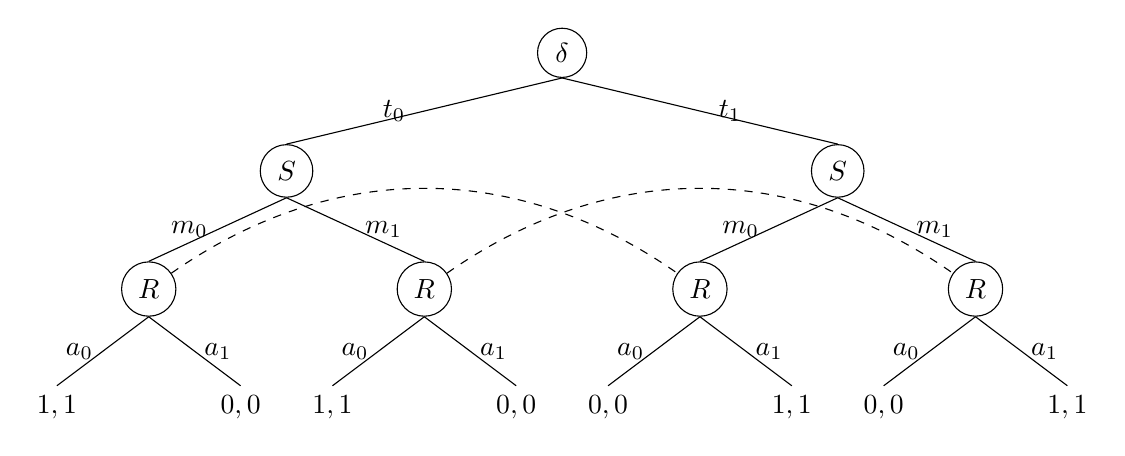
\begin{tikzpicture}[
	scale=1, level/.style={sibling distance=70mm/#1}]
\node  (z)[circle,draw]{$\delta$}
  child {node [circle,draw] (a_left) {$S$}
    child {node  [circle,draw](left_left) {$R$}
      child {node {$1,1$}        
      edge from parent
		node[left] {$a_0$}
		node[right] {}} 
      child {node (n){$0,0$}
      edge from parent
		node[left] {}
		node[right] {$a_1$}}
    edge from parent
	node[left] {$m_0$}
	node[right] {}}
    child {node  [circle,draw](left_right) {$R$}
      child {node {$1,1$}        
      edge from parent
		node[left] {$a_0$}
		node[right] {}} 
      child {node (n){$0,0$}
      edge from parent
		node[left] {}
		node[right] {$a_1$}}
    edge from parent
	node[left] {}
	node[right] {$m_1$}}
  edge from parent
	node[left] {$t_0$ $ $}
	node[right] {}
  }
 child {node [circle,draw] (a_right) {$S$}
    child {node  [circle,draw](right_left) {$R$}
      child {node {$0,0$}        
      edge from parent
		node[left] {$a_0$}
		node[right] {}} 
      child {node (n){$1,1$}
      edge from parent
		node[left] {}
		node[right] {$a_1$}}
    edge from parent
	node[left] {$m_0$}
	node[right] {}}
    child {node  [circle,draw](right_right) {$R$}
      child {node {$0,0$}        
      edge from parent
		node[left] {$a_0$}
		node[right] {}} 
      child {node (n){$1,1$}
      edge from parent
		node[left] {}
		node[right] {$a_1$}}
    edge from parent
	node[left] {}
	node[right] {$m_1$}}
  edge from parent
	node[left] {}
	node[right] {$ $ $t_1$}
  };
\draw [dashed](left_left) to [out=35,in=-215] (right_left);
\draw [dashed](left_right) to [out=35,in=-215] (right_right);
\end{tikzpicture}
\caption{\textbf{Signaling Game:} Two states, messages, and actions. }
\label{SG1}
\end{figure}

As alluded to above, with the exception of the topmost node and the leaves, all other nodes are \emph{decision nodes}. That is, they represent those points in the game where a particular player must make a decision. An \emph{information set} consists of a set of decision nodes for a given player, which that player cannot distinguish. For example, the receiver is in an information set after hearing $m_0$. She is not sure whether she is in the node beneath state $t_0$ or $t_1$ and she must choose between $a_0$ and $a_1$. She is likewise uncertain after receiving message $m_1$. Again, her inability to distinguish the two states is indicated by a dashed line. An information set can also consist of a single decision node. For example, the sender is never uncertain about the state he is in. Thus the information sets for the sender only ever consist of a single node. 

For each player, a \emph{strategy} specifies which action to take at all \emph{information sets} for a player.\footnote{For simplicity, we only consider \emph{pure} sender (receiver) strategies, functions from states to messages (messages to actions). \emph{Mixed} strategies are a straightforward generalization. A mixed sender strategy specifies a probability distribution over pure sender strategies, $\sigma = p_1 s_1 + ... + p_k s_k$, where $\sum_i p_i = 1$. Similarly, a mixed receiver strategy specifies a probability distribution over pure receiver strategies, $\rho = q_1 r_1 + ... + q_k r_k$.} We will refer to the set of all such sender strategies as $S : [T \rightarrow M ]$, and the set of all such receiver as $R : [M \rightarrow A]$. All pure sender and receiver strategies are summarized in Figure \ref{signaling-strategies}. The sender and receiver strategies that combine to yield a one-to-one mapping from states to actions are called \emph{signaling systems}. Thus, the strategy profiles $\langle s_1, r_1 \rangle$ and $\langle s_4, r_4 \rangle$ constitute signaling systems.

\begin{figure}
\begin{center}
\begin{tikzpicture}[->,>=stealth',shorten >=1pt,auto,node distance=2cm]
  \node (A)      {$t_0$};
  \node (B) [right=2cm of A]  {$m_0$};
  \node (C) [below of=A] {$t_1$};
  \node (D) [right=2cm of C] {$m_1$};
\path[->] (A) edge node {} (B)
	  (C) edge node {} (D);
   \node (name) [below left=.5cm and .5cm of A]  {$s_1:$};
   %
     \node (D) [right=3cm of B]   {$m_0$};
  \node (E) [right=2cm of D]  {$a_0$};
  \node (F) [below of=D] {$m_1$};
  \node (G) [right=2cm of F] {$a_1$};
\path[->] (D) edge node {} (E)
	  (F) edge node {} (G);
   \node (name) [below left=.5cm and .5cm of D]  {$r_1:$};
\end{tikzpicture}
\vspace{2cm}

\begin{tikzpicture}[->,>=stealth',shorten >=1pt,auto,node distance=2cm]
  \node (A)      {$t_0$};
  \node (B) [right=2cm of A]  {$m_0$};
  \node (C) [below of=A] {$t_1$};
  \node (D) [right=2cm of C] {$m_1$};
\path[->] (A) edge node {} (B)
	  (C) edge node {} (B);
   \node (name) [below left=.5cm and .5cm of A]  {$s_2:$};
   %
     \node (D) [right=3cm of B]   {$m_0$};
  \node (E) [right=2cm of D]  {$a_0$};
  \node (F) [below of=D] {$m_1$};
  \node (G) [right=2cm of F] {$a_1$};
\path[->] (D) edge node {} (E)
	  (F) edge node {} (E);
   \node (name) [below left=.5cm and .5cm of D]  {$r_2:$};
\end{tikzpicture}\\
\vspace{2cm}

\begin{tikzpicture}[->,>=stealth',shorten >=1pt,auto,node distance=2cm]
  \node (A)      {$t_0$};
  \node (B) [right=2cm of A]  {$m_0$};
  \node (C) [below of=A] {$t_1$};
  \node (D) [right=2cm of C] {$m_1$};
\path[->] (A) edge node {} (D)
	  (C) edge node {} (D);
   \node (name) [below left=.5cm and .5cm of A]  {$s_3:$};
   %
     \node (D) [right=3cm of B]   {$m_0$};
  \node (E) [right=2cm of D]  {$a_0$};
  \node (F) [below of=D] {$m_1$};
  \node (G) [right=2cm of F] {$a_1$};
\path[->] (D) edge node {} (G)
	  (F) edge node {} (G);
   \node (name) [below left=.5cm and .5cm of D]  {$r_3:$};
\end{tikzpicture}\\
\vspace{2cm}

\begin{tikzpicture}[->,>=stealth',shorten >=1pt,auto,node distance=2cm]
  \node (A)      {$t_0$};
  \node (B) [right=2cm of A]  {$m_0$};
  \node (C) [below of=A] {$t_1$};
  \node (D) [right=2cm of C] {$m_1$};
\path[->] (A) edge node {} (D)
	  (C) edge node {} (B);
   \node (name) [below left=.5cm and .5cm of A]  {$s_4:$};
   %
     \node (D) [right=3cm of B]   {$m_0$};
  \node (E) [right=2cm of D]  {$a_0$};
  \node (F) [below of=D] {$m_1$};
  \node (G) [right=2cm of F] {$a_1$};
\path[->] (D) edge node {} (G)
	  (F) edge node {} (E);
   \node (name) [below left=.5cm and .5cm of D]  {$r_4:$};
\end{tikzpicture}\\
\vspace{2cm}


\end{center}
\caption{Sender and Receiver strategies for signaling game}
\label{signaling-strategies}
\end{figure}



The set of possible combinations of sender and receiver strategies constitute \emph{strategy profiles}. That is, a sender strategy in the set of possible sender strategies, $s \in S$, and a receiver strategy in the set of all possible receiver strategies, $r  \in R$, yield a strategy profile $\langle s,r \rangle$. Each strategy profile determines the outcome of the game. Crucially, each player's utility function depends on the state of the sender and the action taken by the receiver. That is, their respective utilities are a function of state and action. As an example, consider the case where both sender and receiver prefer successful communication. Then they both receive their preferred payoffs if there is some correspondence between the sender's state and the receiver's action. For example, in Figure \ref{SG1} both sender and receiver prefer the state and action to be the same in the following sense.

\begin{equation}
 U_{S}(t_i, a_k) = U_{R}(t_i, a_k) =
\left\{
	\begin{array}{ll}
		1  & \mbox{if } i = k \\
		0 & \mbox{else}
	\end{array}
\right.
\end{equation}
Note that this reflects the assumption that both sender and receiver have the same preference over outcomes.

Given that the different states occur with certain probabilities, and we are interested in how particular strategies do on average, we consider the expected utility for a given strategy profile. This is simply the expected value of the utility functions given the two strategies, which can be given in the case of a discrete state space as in our example above.

\begin{equation}
\begin{split}
 E[U_{S}(s,r)] &= \sum_{t} \delta (t) \cdot U_S(t, r(s(t)))\\
 E[U_{R}(s,r)] &= \sum_{t} \delta (t) \cdot U_R(t, r(s(t)))
\end{split}
\end{equation}
For each possible state the sender and receiver strategies determine an outcome. $s(t)$ is the message the sender will employ and $r(s(t))$ is the action the receiver will take given that message. The expected utility is the sum of these outcomes weighted by the probability of the state that yields them. Assuming that the two states are equiprobable, we can construct the payoff matrix for the signaling game as in Table \ref{sig-table}. Since payoffs are symmetric, only one number is presented.

\begin{table}\centering
\begin{tabular}{lllll}
\hline\noalign{\smallskip}
 & $r_1$ & $r_2$ & $r_3$ & $r_4$ \\
\noalign{\smallskip}\hline\noalign{\smallskip}
$s_1$ & $1$ & $\frac{1}{2}$  & $\frac{1}{2}$  & $0$ \\

$s_2$ & $\frac{1}{2}$ & $\frac{1}{2}$  & $\frac{1}{2}$  & $\frac{1}{2}$ \\

$s_3$ & $\frac{1}{2}$ & $\frac{1}{2}$  & $\frac{1}{2}$  & $\frac{1}{2}$ \\

$s_4$ & $0$ & $\frac{1}{2}$  & $\frac{1}{2}$  & $1$ \\

\noalign{\smallskip}\hline
\end{tabular}
\caption{Payoff matrix for signaling game}
\label{sig-table}
\end{table}
There are several Nash equilibria in the game, but only the signaling systems $\langle s_1, r_1 \rangle$ and $\langle s_4, r_4 \rangle$  are evolutionarily stable strategies, because they are the only strict Nash equilibria. In fact, given the structure of the payoffs it is possible to show that these signaling systems are the unique asymptotically stable rest points of the system, which attract the entire interior of the state space \citep[82]{hofbauer-sigmund:1998}. This means that one of the two signaling systems is almost guaranteed to evolve.


%\begin{definition}
% A strategy profile $\langle s^*, r^*\rangle$ is a \emph{Nash equilibrium}
%if and only if:
%  \begin{itemize}
%   \item For all $s \in S$, such that $s \neq s^*$, $E[U_S(s^*,r^*)] \geq
%E[U_S(s,r^*)]$
%  \item For all $r \in R$, such that $r \neq r^*$, $E[U_R(s^*,r^*)] \geq
%E[U_S(s^*,r)]$
%  \end{itemize}
%\end{definition}

%Before I prove the theorems stated in the main text, I will first prove two lemmata that will be used frequently below.
%
%Lemma 10. Let ? be a partnership game with  payoff matrix A. Then:
%
%1.	
% is evolutionarily stable if and only if  is asymptotically stable under the replicator dynamics (1) generated by A.
%2.	
%The replicator dynamics (1) for \Gamma is a Shashshahani gradient system with potential function  .
%Proof. See Hofbauer and Sigmund (1998) p.82. ?
%
%The second part of Lemma 10 implies that all solutions converge to a rest point (Akin and Hofbauer 1982). Moreover, it implies that there are no circling solutions since the average payoff V is strictly increasing along all nonstationary solutions.

\section{Behavioral dynamics}

While the simplest signaling game can be analyzed in a fairly straightforward manner, we might be interested in larger, more complicated games. For example, we might wonder about the dynamics of signaling if the state space were continuous rather than discrete. If we were to approach this by first enumerating all sender and receiver strategies, the dimensions of the system would explode exponentially. One means of controlling for this increase suggested by \cite{hofbauer-huttegger2015} is to consider behavioral strategies insofar as no information is lost in doing so (cf. \citealt{kuhn1953}).\footnote{Erol Ak\c{c}ay (p.c.) has suggested a similar approach to the problem.} The basic idea is that instead of there being a single sender population and a single receiver population, there are multiple sender and receiver populations. Each sender population corresponds to a particular state, and messages compete to be used in that state. Each receiver population corresponds to a message, and actions compete to be used in response to that message.  We start off by defining the components necessary for our analysis. Once we have defined these components we can simulate the game dynamics.


%\begin{itemize}
%	\item The relationship between mixed strategies and behavioral strategies in extensive games of perfect recall is well understood \cite{kuhn1953}. In particular, if one is interested in the equilibrium structure of extensive form games, then no essential information is lost by focusing on behavioral strategies. We propose a similar move for the evolutionary dynamics of signaling games
%%	\item The selection-mutation dynamics in behavioral strategies can be thought of as a dynamics in the entries of the sender and receiver matrices, since these matrices are nothing but a representation of the game�s behavioral strategies.
%	\item A non-injective surjective function: a surjection
%	\item Lose information, condense
%\end{itemize}



%First, we define the payoff matrices for senders and receivers, which depend solely on the utility functions of senders and receivers respectively. $\textbf{A}$ is an $n \times n$ matrix such that $\textbf{A}_{ij} = U_S(t_i, a_j)$:
%
%
%\begin{equation}
%\textbf{A} =
% \begin{pmatrix}
%  U_S(t_1, a_1) & \cdots & U_S(t_1, a_j) & \cdots & U_S(t_1, a_n) \\
%  \vdots	        & \ddots & \vdots           &           & \vdots \\
%  U_S(t_i, a_1) & \cdots & U_S(t_i, a_j) & \cdots & U_S(t_i, a_n) \\  
%  \vdots	        &  & \vdots           &   \ddots        & \vdots \\
%  U_S(t_n, a_1) & \cdots & U_S(t_n, a_j)  & \cdots & U_S(t_n, a_n) \\
% \end{pmatrix}
%\end{equation}
%$\textbf{B}$ is an $n \times n$ matrix such that $\textbf{B}_{ij} = U_R(t_i, a_j)$:
%
%\begin{equation}
%\textbf{B} =
% \begin{pmatrix}
%  U_R(t_1, a_1) & \cdots & U_R(t_1, a_j) & \cdots & U_R(t_1, a_n) \\
%  \vdots	        & \ddots & \vdots           &           & \vdots \\
%  U_R(t_i, a_1) & \cdots & U_R(t_i, a_j) & \cdots & U_R(t_i, a_n) \\  
%  \vdots	        &  & \vdots           &   \ddots        & \vdots \\
%  U_R(t_n, a_1) & \cdots & U_R(t_n, a_j)  & \cdots & U_R(t_n, a_n) \\
% \end{pmatrix}
%\end{equation}
%
%
%Second, we define the sender and receiver populations. $\textbf{X}$ is a stochastic population matrix such that the proportion of the population in $x_i$ using $m_j$ is $x_{ij}$, with $\sum_j x_{ij} = 1$.
%
%\begin{equation}
%\textbf{X} =
% \begin{pmatrix}
%  x_{11} &  x_{12} & x_{13} \\
%  \vdots        & \vdots & \vdots \\
%  x_{i1} &  x_{i2} & x_{i3} \\
%  \vdots	& \vdots    & \vdots \\
%  x_{n1} &  x_{n2} & x_{n3} \\
% \end{pmatrix}
%\end{equation}
% 
%Intuitively, each row corresponds to a given state. Each element in the row corresponds to the proportion of use in that population.  Each row sums to one because the proportion using the various  signals must sum to one.
% 
%$\textbf{Y}$ is a population matrix such that the proportion of the population in $y_i$ responding with action $a_j$ is $y_{ij}$, with $\sum_j y_{ij} = 1$.
%
%\begin{equation}
%\textbf{Y} =
% \begin{pmatrix}
%  y_{11} & \cdots & y_{1j}  & \cdots & y_{1n} \\
%  y_{21} & \cdots & y_{2j}  & \cdots & y_{2n} \\
%  y_{31} & \cdots & y_{3j}  & \cdots & y_{3n} \\
% \end{pmatrix}
%\end{equation}
%
%Again, intuitively, each row corresponds to a given message. Each element in the row corresponds to the proportion of different responses to the message. Each row sums to one because the proportion using the various responses must sum to one.
% 
% 
%The expected utility of sending message $m_j$ in state $t_i$, where $\textbf{Y}^T$ is the transpose of $\textbf{Y}$:
%
%\begin{equation}
%	E [ x_{ij} ] = (\textbf{A}\textbf{Y}^T)_{ij}
%\end{equation}
%
%The average expected utility in a sender population $x_i$:
%
%\begin{equation}
%	E [ x_{i} ] = (\textbf{X}(\textbf{A}\textbf{Y}^T)^T)_{ii}
%\end{equation}
%
%This gives the replicator dynamic for a given message in a sender population.
%\begin{equation}
%	\dot{x}_{ij} = x_{ij}((\textbf{A}\textbf{Y}^T)_{ij} - (\textbf{X}(\textbf{A}\textbf{Y}^T)^T)_{ii})
%\end{equation}
%
%
%
%
%$\textbf{P}$ is a stochastic matrix such that $\forall i \textbf{P}_i = P(t_1),...,P(t_n)$. That is, $\textbf{P}$ is just $n$ rows of the prior probability distribution over states.
%
%\begin{equation}
%\textbf{P} =
% \begin{pmatrix}
%  P(t_1) & \cdots & P(t_i)  & \cdots & P(t_n) \\
%  \vdots &  & \vdots  & & \vdots  \\
%  P(t_1) & \cdots & P(t_i)  & \cdots & P(t_n) \\
% \end{pmatrix}
%\end{equation}
%
%
%Now that we have defined the  replicator dynamics for the sender populations, we can do the same for the receiver populations with a few additions. Let $\textbf{C}$ be the conditional probability of a state given a message. That is, $\textbf{C}_{ij} = P(t_i | m_j)$, where $\otimes$ indicates element-wise Hadamard multiplication and $\oslash$ indicates the element-wise Hadamard division.
%
%\begin{equation}
%\textbf{C} = (P^T \otimes X) \oslash (PX)
%\end{equation}
%
%
%The expected utility of receiver responding to message $m_i$ with action $a_j$:
% 
%\begin{equation}
%	E [ y_{ij} ] = (\textbf{B}^T\textbf{C})_{ji}
%\end{equation}
%
%Since the resulting matrix is $n \times m$, we swap the indices to get the appropriate value. Each column corresponds to a receiver population, and each row corresponds to a response action.
%
%The average expected utility in a receiver population $y_i$:
%
%\begin{equation}
%	E [ y_{i} ] = (Y(\textbf{B}^T\textbf{C})_{ji})_{ii}
%\end{equation}
%
%The replicator dynamic for a given action in response to a message is given by the following.
%
%\begin{equation}
%		\dot{y}_{ij} = y_{ij}(\textbf{B}^T\textbf{C})_{ji} - (Y(\textbf{B}^T\textbf{C})_{ji})_{ii})
%\end{equation}
%Together these behavioral replicator dynamics can be used to investigate any signaling game with a finite number of states, messages, and actions.

\subsection{The Simplest Signaling Game}

To begin, we apply this new framework to the simplest non-trivial signaling game where we have two equiprobable states, two messages, and two actions. The structure of the behavioral  replicator dynamics is determined by the structure in Figure \ref{behavioral-dynamics}. $x_0$ represents the probability that $m_0$ will be used in the $t_0$ sender population. Likewise $x_1$ represents the probability that $m_1$ will be used in the $t_1$ sender population. The dotted lines indicates probabilities that can be derived from others. All told, then, the behavioral replicator dynamic  for this signaling game gives rise to a four-dimensional system.

\begin{figure}
\begin{center}
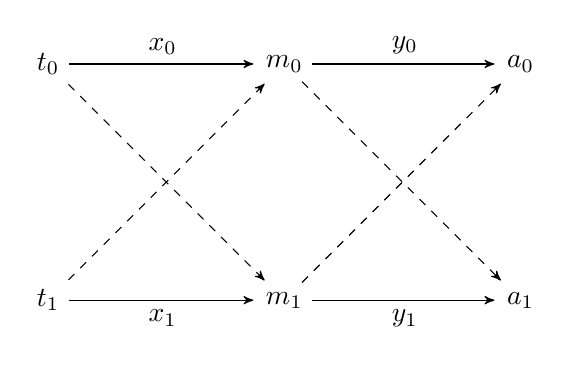
\begin{tikzpicture}[->,>=stealth',shorten >=1pt,auto,node distance=3cm]
  \node (A)      {$t_0$};
  \node (B) [right of=A]  {$m_0$};
  \node (C) [right of=B] {$a_0$};
  \node (D) [below of=A] {$t_1$};
  \node (E) [right of=D] {$m_1$};
  \node (F) [right of=E] {$a_1$};
\path[->] (A) edge node {$x_0$} (B)
	  (A) edge[dashed,pos=0.85] node {} (E)
	  (B) edge node {$y_0$} (C)
	  (B) edge[dashed,pos=0.85] node {} (F)
	  (D) edge[below] node {$x_1$} (E)
	  (D) edge[dashed,pos=0.75] node {} (B)
	  (E) edge[below] node {$y_1$} (F)
	  (E) edge[dashed,pos=0.75] node {} (C);
\end{tikzpicture}
\end{center}
\caption{Signaling game in behavioral space}
\label{behavioral-dynamics}
\end{figure}

We will generalize the parameters a bit to match the simpler games we used above. Namely, let the sender and receiver payoffs be the following matrices, with parameters $\alpha$ and $\beta$.

\begin{equation}
\mathbf{A} =
 \begin{pmatrix}
  1 - \alpha & \alpha \\
  \beta & 1 - \beta \\
 \end{pmatrix}
\end{equation}

\begin{equation}
\mathbf{B} =
 \begin{pmatrix}
  1 & 0 \\
  0 & 1 \\
 \end{pmatrix}
\end{equation}
These yield the general behavioral sender and receiver replicator dynamics.

\begin{equation}
	\begin{split}
		\dot{x}_0 &= x_0(1-x_0)(y_0 + y_1 - 1)(1 - 2\alpha)\\	
		\dot{x}_1 &= x_1(1-x_1)(y_0 + y_1 - 1)(1 - 2\beta)\\
	\end{split}
\end{equation}

\begin{equation}
	\begin{split}
		\dot{y}_0 &= y_0(1 - y_0)\left(\frac{x_0 + x_1 - 1}{x_0 - x_1 + 1}\right)\\
		\dot{y}_1 &= y_1(1 - y_1)\left(\frac{x_0 + x_1 - 1}{x_1 - x_0 + 1} \right)\\
	\end{split}
\end{equation}

 The case where $\alpha = \beta = 0$ corresponds to the lewis signaling game we introduced in the previous section, which is also related to the coordination game we started with. This is a signaling games with common interests. The case where $\alpha = \beta = 1$ corresponds to signaling with matching pennies. This is a signaling game with conflicting interests.  The cases where $\alpha = 0, \beta = 1$  and $\alpha = 1, \beta = 0$ also offer an interesting comparison. These are games of at least partial common interest. We address each of these below.

\subsection{Common Interests}

Since the receiver dynamics do not vary as we change the parameters, we omit them. Under common interests the sender dynamics are the following.

\begin{equation}
	\begin{split}
		\dot{x}_0 &= x_0(1-x_0)(y_0 + y_1 - 1)\\	
		\dot{x}_1 &= x_1(1-x_1)(y_0 + y_1 - 1)\\
	\end{split}
\end{equation}

Typical results for a numerical solution are shown in Figure \ref{common-interests}, where we plot $x_0$ against $y_0$ and $x_1$ against $y_1$, with circles represent the starting state of both of trajectories. That is, we represent the four-dimensional system as two two-dimensional systems overlaid on each other. The established result is exactly what we see. Namely, the system either converges to the origin or to the upper right-hand corner. Referring back to Figure \ref{behavioral-dynamics} it is clear that these constitute the signaling systems of the signaling game as we described them. That is, these are the points that guarantee a one-to-one mapping between states and actions.


\begin{figure}
	\includegraphics{common-interests.pdf}
	\label{common-interests}
	\caption{Solution trajectories for behavioral replicator dynamics for common interest signaling}
\end{figure}


%\begin{equation}
%	\mathbf{J} 
%	 =
%	 \begin{bmatrix} 
%	(- 2 x_{0} + 1) (y_{0} + y_{1} - 1) & 0 & x_{0} (- x_{0} + 1) & x_{0} (- x_{0} + 1)\\
%	0 & (- 2 x_{1} + 1) (y_{0} + y_{1} - 1) & x_{1} (- x_{1} + 1) & x_{1} (- x_{1} + 1)\\
%	\frac{2 y_{0} (x_{1} - 1) (y_{0} - 1)}{(x_{0} - x_{1} + 1)^{2}} & - \frac{2 x_{0} y_{0} (y_{0} - 1)}{(x_{0} - x_{1} + 1)^{2}} & \frac{(- 2 y_{0} + 1) (x_{0} + x_{1} - 1)}{x_{0} - x_{1} + 1} & 0 \\
%	- \frac{2 x_{1} y_{1} (y_{1} - 1)}{(- x_{0} + x_{1} + 1)^{2}} & \frac{2 y_{1} (x_{0} - 1) (y_{1} - 1)}{(- x_{0} + x_{1} + 1)^{2}} & 0 & \frac{(- 2 y_{1} + 1) (x_{0} + x_{1} - 1)}{- x_{0} + x_{1} + 1}\\
%	 \end{bmatrix}
%\end{equation}
%
%It's clear that both $\frac{\partial \dot{y}_0}{\partial x_0}$ and $\frac{\partial \dot{y}_1}{\partial x_0}$ go to infinity as we approach points at the edge of the state space.

%\begin{figure}
%	\includegraphics[width=.5\textwidth]{lewis-phase-portrait-senders}	\includegraphics[width=.5\textwidth]{lewis-phase-portrait-receivers}		
%\end{figure}


\subsection{Conflicting Interests}

If we alter the payoff structure to reflect that of matching pennies, then the following behavioral sender dynamics result.
\begin{equation}
	\begin{split}
		\dot{x}_0 &= x_0(1-x_0)(1 - y_0 - y_1)\\	
		\dot{x}_1 &= x_1(1-x_1)(1 - y_0 - y_1)\\
	\end{split}
\end{equation}

Typical results for numerical solution are shown in Figure \ref{conflicting-interests}. Interestingly, much like in the case of matching pennies, the system exhibits closed orbits.

\begin{figure}
	\includegraphics{conflicting-interests.pdf}
	\label{conflicting-interests}
	\caption{Solution trajectories for behavioral replicator dynamics for conflicting interest signaling}
\end{figure}

An interesting consequence of this behavior is that despite the fact that the sender does not want to signal what action he is going to take, there is some amount of information carried by the signal. This can quantified by calculating the \emph{Kullback-Leibler divergence} or \emph{information gain} due to the signal.

\begin{equation}
	KL(m) = \sum_t P(t \mid m) log \left( \frac{P(t \mid m)}{P(t)} \right)
\end{equation}
The basic intuition behind this formula is that it allows us a way to compare the receiver's expectations prior to receiving the message, which is determined by the probability distribution over states, to the posterior distribution after having heard the message.  The difference between these two distributions is the information gained by having received the message. The average information gain for the two signals is shown in Figure \ref{conflicting-interests-KL}. As a point of reference, if the messages perfectly corresponded to states, as they do in a signaling system, then the average information gain would be equal to one. In other terms, the information gained from the signal would be one bit, because it would allow us to distinguish between two equiprobable states.s

\begin{figure}
	\includegraphics{conflicting-interests-KL.pdf}
	\label{conflicting-interests-KL}
	\caption{Average Kullback-Leibler Divergence for signals under conflicting interests}
\end{figure}

The fact that signals still carry information, even under diametrically opposed interests is both interesting and surprising (cf. \citealt{sato-etal2002,wagner2012}).

%\subsection{Partial Common Interests}
%
%Perhaps even more surprising is the case of only partially misaligned interests, or as \cite{blume-etal:2001} refer to them, \emph{partial common interests}. That is, when $\alpha = 0, \beta = 1$  and $\alpha = 1, \beta = 0$, then at least some of the time senders want to accurately signal their type. Consider the case where $\alpha = 1, \beta = 0$, which yields the following behavioral dynamics.
%
%\begin{equation}
%	\begin{split}
%		\dot{x}_0 &= x_0(1-x_0)(1 - y_0 - y_1)\\	
%		\dot{x}_1 &= x_1(1-x_1)(y_0 + y_1 - 1)\\
%	\end{split}
%\end{equation}
%
%\begin{figure}
%	\includegraphics{partial-common-interests.pdf}
%	\label{partial-common-interests}
%	\caption{Solution trajectories for behavioral replicator dynamics for partial common interest signaling}
%\end{figure}
%
%Typical results for a numerical solution are presented in Figure \ref{partial-common-interests}. The sender populations converge to opposite sides of the state space, meaning that senders all converge on using the same signal. In response to this, receivers converge to some intermediate response, although not necessarily the one that might be expected from the distribution over states. The most striking thing about this case is that it differs dramatically from the case where interests are perfectly opposed. In the first case no information is carried by the messages, whereas there is always some information carried by messages in the second.


\section*{Summary}

In this chapter we outlined the basic framework that will be used subsequently. We noted the complementary role of static and dynamic methods for understanding the evolution of populations. We also presented a general method for describing the dynamics of signaling games and noted interesting properties of the simplest kind of signaling game. We now turn to our application of this framework to the functional Jespersen cycle.

% Cycles
\chapter{Cycles (30 pages)}
\label{Cycles}

\epigraph{"I don't know what you mean by 'glory,'?" Alice said.

Humpty Dumpty smiled contemptuously. "Of course you don't -- till I tell you. I meant 'there's a nice knock-down argument for you!'?"

"But 'glory' doesn't mean 'a nice knock-down argument'," Alice objected.

"When I use a word," Humpty Dumpty said, in rather a scornful tone, "it means just what I choose it to mean -- neither more nor less."

"The question is," said Alice, "whether you can make words mean so many different things."

"The question is," said Humpty Dumpty, "which is to be master, that's all."

--Lewis Carroll\\

I can't say `It's cold here' and mean `It's warm here' -- at least, not without a little help from my friends.\\--David Lewis}


We are now in a position to bring the formal framework developed in Section \ref{Signaling} to bear on the use of emphatic negation and its role in Jespersen's Cycle. We begin by first mapping the components discussed in Section \ref{Background} onto the structure of a signaling game. The possibility of different preferences for speakers and hearers is incorporated into the structure of the model. We determine the existence of evolutionarily stable strategies and note the transfer of information as the interests of speaker and hearer diverge. As the preferences of speakers and hearers diverge signaling becomes less informative. For sufficiently low differences, signaling remains informative, but beyond a certain point signaling collapses into uninformative pooling. We then consider the impact of introducing new signals, which lead to a kind of push-chain where the least informative signal is lost. Throughout, we discuss the implications of the model for Jespersen's Cycle.

\section{Emphasis}

\subsection{Signaling Game}

To begin, we must first consider how signaling games capture the use of negation. As we noted above, the difference between plain and emphatic negation is captured by the standard of precision applied. The speaker has knowledge about some state of the world which renders a particular negative expression acceptable on some standards, but not necessarily on others. Thus, there exists a continuum of states for the speaker, which we will take to be the interval $T = [0,1]$. The lowest possible value on such an interval corresponds to the weakest possible standard of precision that would still render the negative expression acceptable.\footnote{Here we leave out the possibility of the use of a given expression in the absence of any standard of precision being met. That is, we leave out cases of outright lying. Such cases are particularly interesting, but we leave them as a consideration for future study.} The highest possible value on the interval is then the strictest possible standard of 
interpretation available. 

Given that the speaker has observed some state of affairs, $t \in T$, he must choose a message, $m \in M$, to send to the hearer. Let $\mathcal{P}_n(T)= 0 < ... < t_{n-1} < ... < 1$ be a partition of the state space into $n$ subintervals.  A speaker's strategy is then a function from a partition of the type space to messages, $S : [\mathcal{P}_n(T) \rightarrow M]$. Intuitively, this is simply a way of carving up the state space into discrete regions and using those regions to determine which signal to send. For example, the trivial partition, $\mathcal{P}_1(T)$, occurs when the sender pools all types together and uses only a single message. In what follows we will largely be concerned with partitions of at least size two $\mathcal{P}_2(T)$. For example, consider the case of two messages, consisting of just a plain and an emphatic form. Letting $\mathcal{P}_2(T) = 0 < t_1 < 1$, a possible sender strategy is then  $s(t) = m_1$ for $t \in (0,t_1)$, and $s(t) = m_2$ for $t \in (t_1,1)$. That is, the sender uses 
$m_1$ for all types in the first subinterval, and $m_2$ for the second subinterval. Intuitively, we would refer to $m_1$ as the plain form of negation and $m_2$ as the emphatic.

Once the speaker has sent a message, the hearer is faced with the problem of how to interpret it. Given that the hearer cannot read the speaker's mind, she must infer the state of affairs that prompted the use of a particular form. That is, given the information conveyed by the signal, she must do her best to determine the standard of precision that warrants the speakers assertion. We will take the space of possible interpretations available to the hearer to be equivalent to the type space of the speaker, $A = [0,1]$. This representation captures the fact that the interpretation of expressions is not an all or nothing affair, but rather a matter of degrees.  A hearer's strategy is then a mapping from messages to interpretations, as above, $R : [M \rightarrow A]$.


\begin{figure}
\begin{center}
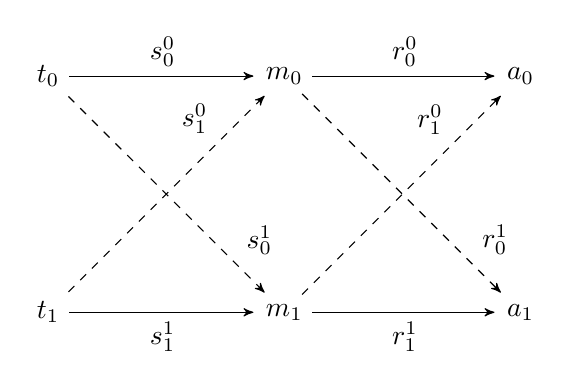
\begin{tikzpicture}[->,>=stealth',shorten >=1pt,auto,node distance=3cm]
  \node (A)      {$t_0$};
  \node (B) [right of=A]  {$m_0$};
  \node (C) [right of=B] {$a_0$};
  \node (D) [below of=A] {$t_1$};
  \node (E) [right of=D] {$m_1$};
  \node (F) [right of=E] {$a_1$};
\path[->] (A) edge node {$s_0^0$} (B)
	  (A) edge[dashed,pos=0.85] node {$s_0^1$} (E)
	  (B) edge node {$r_0^0$} (C)
	  (B) edge[dashed,pos=0.85] node {$r_0^1$} (F)
	  (D) edge[below] node {$s_1^1$} (E)
	  (D) edge[dashed,pos=0.75] node {$s_1^0$} (B)
	  (E) edge[below] node {$r_1^1$} (F)
	  (E) edge[dashed,pos=0.75] node {$r_1^0$} (C);
\end{tikzpicture}
\end{center}
\caption{Probabilities of actions in signaling game}
\label{probs}
\end{figure}

\begin{figure}
\begin{center}
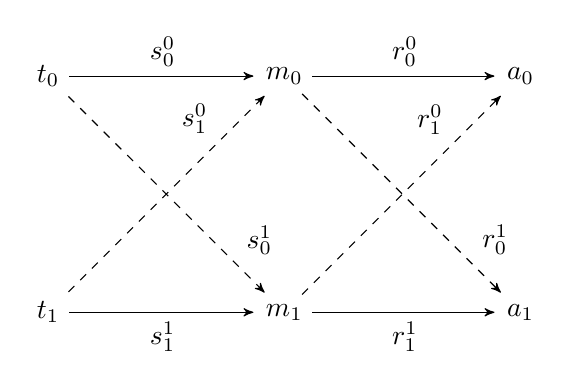
\begin{tikzpicture}[->,>=stealth',shorten >=1pt,auto,node distance=3cm]
  \node (A)      {$t_0$};
  \node (B) [right of=A]  {$m_0$};
  \node (C) [right of=B] {$a_0$};
  \node (D) [below of=A] {$t_1$};
  \node (E) [right of=D] {$m_1$};
  \node (F) [right of=E] {$a_1$};
%  \node (G) [below of=D] {$t_2$};
\path[->] (A) edge node {$s_0^0$} (B)
	  (A) edge[dashed,pos=0.85] node {$s_0^1$} (E)
	  (B) edge node {$r_0^0$} (C)
	  (B) edge[dashed,pos=0.85] node {$r_0^1$} (F)
	  (D) edge[below] node {$s_1^1$} (E)
	  (D) edge[dashed,pos=0.75] node {$s_1^0$} (B)
	  (E) edge[below] node {$r_1^1$} (F)
	  (E) edge[dashed,pos=0.75] node {$r_1^0$} (C);
\end{tikzpicture}
\end{center}
\caption{Probabilities of actions in signaling game}
%\label{probs}
\end{figure}



With the definition of the strategies available to speakers and hearers, we can ask what kinds of preferences both might have over the correspondence between actual and inferred standards. It is uncontroversial that hearers are in the business of doing their best to accurately infer the actual state of affairs that prompted the signal. That is, hearers prefer their interpretation to be as close as possible to the standard of precision that the speaker actually has evidence for.  If it were otherwise, the existence of language would be truly puzzling from an evolutionary perspective; the gullible are not long for the tooth and claw world. So, if hearers are interested in the accurate transmission of information, then any misalignment must come from speakers' preferences. 

From the perspective of the speaker, we can adduce at least two related reasons why speakers might prefer overestimation. The first imputes a kind of categorical bias on the part of speakers, whereas the second relaxes this bias towards reasonability. We address them each in turn. First, we consider what the goals of communication are. Arguably, our chief goal in uttering a given expression is to affect some response in our interlocutors. In the case of a declaration we might think of this in terms of how convinced the hearer is after hearing an utterance. Or, in the terms we have developed thus far, we want the hearer to infer a particular standard of precision. We could take this preference as categorical. Namely, that regardless of the actual standard of precision, speakers want hearers to infer the absolute highest standard of precision possible. Given such a preference and a choice between signals that hearers respond to differentially, speakers will always choose the form that elicits the higher 
standard.  Speakers are, so to speak, on the lookout for the form that gives them the most bang for their breath. It should be noted that this bias is stipulative only insofar as it arises from the fundamental way we use words to do things.

Second, while this bias may naturally exist, it need not be categorical. Rather, speakers may simply prefer that hearers infer a standard of precision that is at least is strict as their own. This can be taken as a natural corollary of the inferential nature of communication. Hearers cannot read minds, and thus they must make some inference about the actual standard of precision. Speakers have only an indirect influence on this process of inference. Thus, they may wish to hedge their bets in a particular direction. Namely, they may want the inferred standard to be at least as strict as there own because it ensures that their own beliefs stand in a particular relation to hearers'. That is, the hearer's beliefs probabilistically entail those of the speaker.

The impact of this relationship is particularly clear with regard to perlocutionary concerns. For example, imagine the case where the issuer of one of the following threats has absolutely no desire to follow through on it.

  \ex. \a. If you move, I'll shoot.
       \b. If you budge an inch, I'll shoot.

By using the stronger threat, leading the hearer to infer a stricter standard than actually holds, the speaker has a better chance of not being forced to follow through on it. That is, the hearer will restrict his actions to those that do not constitute movement at the stricter standard, thus guaranteeing that they will not at the weaker actual standard. 

The same concerns hold in far more magnanimous circumstances. For example, in the case of offering a friend genuine advice on dining options, one might deem a mediocre restaurant one of the following.

 \ex. \a. Not good.
      \b. Not worth a cent!

While clearly hyperbole, the latter, much like the strong threat, offers a means for speakers to guide a friend to a good meal. In both cases, when hearers underestimate the standard of precision, the speaker runs the risk of not achieving his goals with resulting dire or not so delicious consequences. In contrast, these goals are guaranteed when hearers overestimate the standard of precision.

We can encode this slight bias in the utility functions of senders and receivers. As a means of parameterizing this possibility, we define the sender and receiver utility functions as a pair of quadratic functions, as in \cite{crawford-sobel:1982}, where $b \in [0,1]$ reflects the bias of the sender.\footnote{This bias need not be constant. For example, we might suppose that the bias is uniformly distributed over the interval $(t,t+b)$. This would capture the intuition that some of the time a speaker prefers overestimation of the standard, but not others. All of the following result hold for this more general case. As a preview, the only change below is that partial pooling equilibrium is defined at $t^* = \frac{1}{2} - 3b$ }

\begin{equation}
\begin{split}
     U_S(t, a) &= -(a - t - b)^2\\
  	 U_R(t, a) &= -(a - t)^2
\end{split}
\end{equation}
These utility functions reflect two intuitions. First, for a given type of sender, there is an action that maximizes the receiver's payoff. That is, the receiver does best by taking the action that is closest to the sender's type. Second, for a sender with a particular type, the action that maximizes the sender's payoff is offset by some bias, $b$. That is, the sender prefers the receiver to take the action she thinks appropriate for some higher type. In this case, $b$ represents the degree to which the sender wishes to exaggerate his type, if the receiver believes such exaggerations. When $b=0$ the interests of senders and receivers are completely aligned, but as $b$ grows, they diverge. This parallels the intuition that hearers are trying to infer the standard of precision for a given assertion, and prefer this to be as accurate as possible. It also reflects the fact that speakers have a slight preference for hearers to overestimate the standard of precision.

The impact of the sender's bias can be visualized as in Figure \ref{receiver_payoff}. For a sender with information $t=0$, the receiver would do best to take the action that accurately picks out the sender's state. In contrast, the sender's most preferred action is offset by the amount of bias. In the case where $b=\frac{1}{2}$, then the sender prefers the speaker to take an action higher than the receiver would prefer. This mismatch is only exacerbated as the amount of bias increases, as can be seen for the case where $b=1$. Visually speaking, as the bias increases, the utility functions of the sender and the receiver move away from each other. 


\begin{figure}
\begin{center}
\begin{tikzpicture}
\node (left) at (-1, 2)    {\includegraphics[width=.15\textwidth]{left.jpg}};
%draw horizontal line
\draw (0,0) -- (6,0);
%draw ticks
\draw (0,3pt) -- (0,-3pt);
\draw (6,3pt) -- (6,-3pt);
%draw tick labels
\draw (0,0) node[below=3pt] {\textsc{discourse new} } ;
\draw (6,0) node[below=3pt] {\textsc{discourse old} } ;
%
\draw (3,3pt) -- (3,-3pt);
\node (state) at (3, 1)    {$t$};
%
\draw (5,3pt) -- (5,-3pt);
\node (state) at (5, 1)    {$t+b$};
\draw [ultra thick] (3,1.5) to (5,1.5);
\node (state) at (4, 1.75)    {$b$};
\end{tikzpicture}     
\end{center}
\caption{$p :$ The plumber came.}
\end{figure}

\subsection{Equilibria}

For a given pair of sender and receiver strategies we can calculate the expected utility. In what follows we will assume that types are uniformly distributed over the interval, which yields the following expected utilities. Note that these are exactly parallel to expected utilities in a discrete state space presented above.

\begin{equation}
\begin{split}
     E[U_S(s, r)] &= \int_T -(r(s(t)) - t - b)^2 dt\\
      E[U_R(s, r)] &= \int_T -(r(s(t)) - t)^2 dt
\end{split}
\end{equation}

Now, we want to determine the conditions for equilibria. By doing so, we are determining what kinds of behavior we would expect on the part of speakers and hearers given the speaker's bias. That is, we want know how speakers will use different forms to signal standards of precision and how hearers will interpret them. The existence of different equilibria and their relative stability are crucial to the dynamics of Jespersen's Cycle.

Consider the potential equilibrium strategy profile $\langle s^*, r^* \rangle$. Let $s^*$ induce a partition of type $\mathcal{P}_2(T)$, where $t^*$ is the relevant threshold that distinguishes the two messages. Let $s^*(t) = m_1$ for $t \in (0,t^*)$ and $s^*(t) = m_2$ for $t \in (t^*,1)$. Let $r^*(m_1) = a_1^*$ and $r^*(m_2) = a_2^*$. In words, the sender splits the type space in two and sends a unique message for each subinterval. These are the plain and the emphatic forms of negation, respectively. The receiver responds to these messages with a particular action.  These are the inferred standards of precision in response to the different forms.

The strategy profile is an equilibrium if the relevant strategies are joint best responses. We can determine this by simply taking the partial derivative of the relevant utility functions with regard to the relevant variables. For the receiver, this can be determined by considering what actions are the best response to the senders partition. This simply tells us how the receiver's inference depends on the sender's use of the different forms.

\begin{equation}
\frac{\partial}{\partial a_1^*}E[U_R(s, r)] = \frac{\partial}{\partial a_2^*}E[U_R(s, r)] = 0
\end{equation}
These values are uniquely satisfied when the following hold.

\begin{equation}
     \begin{split}
	  a_1^* &= \frac{t^*}{2}\\
	  a_2^* &= \frac{1 + t^*}{2}
     \end{split}
\end{equation}
Intuitively, this means that however the speaker splits up the standards of precision, the receiver should respond to the emphatic form by inferring a higher standard of precision and the plain form with a lower standard of precision. The exact placement of these responses is determined by how the sender uses the signals. Namely, the hearer should infer the average standard of precision used for each of the two forms.

For the sender, we can proceed in a similar fashion determining when the following holds.
\begin{equation}
 \frac{\partial}{\partial t^*}E[U_S(s, r)] = 0
\end{equation}
This equation is satisfied when one of the following holds.

\begin{equation}
     \begin{split}
 	t^* &= 0\\
	t^* &= \frac{3}{4}(a_1^* + a_2^*) - \frac{3}{2}b - \frac{1}{4}\\
	t^* &= 1
     \end{split}
\end{equation}

These constraints together give rise to three distinct systems of equation. Solving each for $t^*$, we find the following equilibrium solutions in terms of the bias of the sender.

\begin{equation}
\begin{split}
     t^* &= 0\\
     t^* &= \frac{1}{2} - 6b\\
     t^* &= 1
\end{split}
\end{equation}
Both the first and the last of these equilibria are pooling equilibria. That is, senders only ever use a single signal. In response to this, receivers take the action that maximizes their expected utility given the prior probability distribution over types. That is, they guess the expected value of the type space. They simply infer the average standard of precision.

In contrast, the middle equilibrium constitutes a partially separating equilibrium. It is only partially separating because the state space is infinite, while the message space is not. This means that every type cannot be fully revealed, but that some information is transferred. The amount of information transferred and the distinction between the partially separating and pooling equilibria can be characterized in information-theoretic terms \citep{shannon:1948}. In particular, we can think of the amount of information conveyed by a particular signal at equilibrium according to the \emph{Kullback-Leibler Divergence} \citeyearpar{kullback-leibler1951divergence}.

\begin{equation}
     D_{KL}(P || Q) = \int_{-\infty}^{\infty} log\left( \frac{p(x)}{q(x)}  \right)p(x) dx
\end{equation}
This serves as a measure for how much change is induced in the receiver by a particular message. That is, in our case $q(x)$ corresponds to the prior probability distribution over types, and $p(x)$ corresponds to the probability of a sender being of a particular type given the message. The more the message shifts the probability from the prior, the more information it conveys. And, the less a message shifts the probability from the prior, the less information it conveys. 

For example, taking either of the pooling equilibria as an example.  If senders use the same signal regardless of state, then the conditional probability is the same as the prior probability. This means that there is absolutely no change from the prior probability, and hence zero information is transmitted via the signal. In contrast, for any partially separating equilibrium, a particular message induces a shift from the prior probability, and thus conveys some information. We should note that the amount of information conveyed regarding the standard of precision is distinct from the propositional content of a given utterance. For example, in the case where speakers use only a single form of negation for all standards of precision, the hearer will have no information in addition to and exceeding the prior probability. However, she will know the propositional content of the utterance. In other words, she will know \emph{that} negation was used, but not \emph{how} it was used.


Information is transferred at equilibrium only if the partially separating equilibrium exists. This is the case when the sender's bias is sufficiently low. Namely, only if $b < \frac{1}{12}$. If the bias is too large, then the partially separating equilibrium collapses into the lower pooling equilibrium.  However, a partially separating equilibrium, if it exists, is the only evolutionarily stable strategy profile. To see this note that in any pooling equilibrium receivers can respond to an unused message with any action whatsoever without affecting their expected utility. This means that pooling equilibria are not strict Nash equilibria and are thus not stable to invasion or innovation. 

% For example, suppose that receivers responded to an unused message with an action $a > \frac{1}{2}$. All senders would then do better to use that previously unused message in a particular set of states, $(\frac{1}{2}(a + \frac{1}{2}), 1]$. In turn, receivers woul
% 
%  have an incentive to adjust their responses to the two messages. In turn, senders have an incentive to adjust to this adjustment, and so forth. This process of mutual adjustment ends at the evolutionarily stable partially separating equilibrium.

We have established an upper limit on the amount of bias that allows for two signals to be used informatively. If this bias is exceeded, then signaling collapses. A single message is used, but carries no information. In fact, for a given number of signals, $n$, there exists some level of bias, $b_n$, that allows for their informative use in a partially separating equilibrium based on a sender's partition of the type space, $\mathcal{P}_n$ \citep{crawford-sobel:1982}. As the number of signals increase, the amount of bias must decrease to allow for informativity, thus $b_2 > b_3 > ... > b_n$. Intuitively, as the preferences of senders and receivers approach each other a finer and finer partition of the space is possible.

\subsection{Dynamics}

So, what does this mean for Jespersen's cycle? Intuitively, the pragmatics of emphasis suggest that the population originally starts at a point where one form is used with a  very high standard of precision and another is used for all other standards. That is, emphatic negation is distinguished from plain negation in its contexts of use. We can determine what will happen to these two signals over time. Intuitively, under the game dynamics, the signals will converge to their equilibrium use.

Under the game dynamics, for any amount of bias, no matter how slight, the emphatic form will spread to lower and lower standards of precision until it reaches its equilibrium use. The amount of bias determines where this process stops. That is, if a partially separating equilibrium exists, then the emphatic form will expand to encompass all standards of the upper part of the partition. In other words, the emphatic will be \emph{attenuated}, but still carry some information.  If no separation is possible, the emphatic form will spread across all standards. In other words, the emphatic will be entirely \emph{bleached} of its emphasis. Note that in both cases the process can be characterized in information-theoretic terms. That is, as the emphatic form spreads to more and more standard it conveys less and less information. 

The stable coexistence of plain and emphatic negation for long periods of time suggest that the bias is sufficiently small to allow for at least two forms. This, however, raises the question of what destabilizes the system. The system must be disturbed by a push chain, whereby the signal used for the lowest subinterval is lost. More generally, imagine a system with bias $b_n$ at equilibrium. Now, suppose that a new signal is introduced, so that there are now $n+1$ signals. Clearly, the system is not stable. However, it will be carried back to some equilibrium by the game dynamics. The resultant equilibrium depends on the character of the signal that is introduced. Let $a'$ be the response of receivers to the new signal $m'$. All messages that receive a lower response than $a'$ will be pushed down, the lowest of these being pushed out of use completely.  In the case of Jespersen's Cycle, new signals enter with a high $a'$, and thus displace everything below. That is, they are emphatic and lead hearers to 
infer a high standard of precision. This means that all other forms lower in the scale will be pushed down and the lowest will be pushed out of existence, exactly like what we see in the actual instantiation of the cycle.

\subsection{Modeling}

\begin{figure}
\centering
     \includegraphics[width=\textwidth]{lump-plot1.pdf}
\caption{Proportion of \textit{\color{blue} ne...not} and \textit{\color{green} not}  versus  \textit{\color{red}  ne} over time}
\label{lump-plot1}
\end{figure}

\begin{figure}
\centering
     \includegraphics[width=\textwidth]{neg-year-lines.pdf}
\caption{Proportion of forms of negation in Negative Declaratives}
\label{neg-three-plot}
\end{figure}


\section{Information Structure}

The motivation of this project stems from particular hypotheses about the conditioning factors of negation in Jespersen's Cycle \citeyearpar{jespersen:1917}, which can be characterized by the transition from pre-verbal to embracing to post-verbal negation: \textsc{\color{red} neg V} $\rightarrow$ \textsc{\color{blue} neg V neg} $\rightarrow$ \textsc{\color{green} V neg}. In particular, \cite{hansen2009, hansen-visconti2009,hansen-visconti2012} have used historical corpora of French and Italian to show that the embracing form (\textsc{\color{blue} neg V neg}) is sensitive to the discourse status of the proposition being negated. Namely, the embracing form is restricted to instances where the proposition being negated is either \textsc{discourse old} or \textsc{inferrable}.

\cite{schwenter2005,schwenter2006} uses synchronic data from Brazilian Portuguese to demonstrate the sensitivity of negation to these distinctions. Consider the following scenario. Suppose that a husband and wife expect a plumber to come fix their leaky faucet while they are at work during the day. The husband arrives home before his wife to find a still leaky faucet. The wife arrives home shortly and the first thing her husband says is the following.

\exg.  O bombeiro \textsc{\color{red} n{\~a}o} \textsc{\color{red} Veio}.\\
         The plumber neg came\\
         ``The plumber didn't come."\\

\exg. \#O bombeiro \textsc{\color{blue}n{\~a}o} \textsc{\color{blue}Veio} \textsc{\color{blue}n{\~a}o}.\\
	The plumber neg came neg\\
	``The plumber didn't come."\\

The reason that the embracing form is odd is that it comes out of the blue, so to speak. That is, the proposition ``The plumber came.'' is entirely \textsc{discourse new}. Even if the husband has some expectation that his wife has been thinking about whether or not the plumber came, the proposition has not been introduced into the \emph{discourse} yet. The embracing form cannot be used to negate \textsc{discourse new} propositions.

However, how the proposition can be introduced into the discourse in several ways, both explicitly and implicitly. For example, if the wife walks in the door and says the following.

\exg.  O bombeiro veio hoje?\\
       The plumber came today\\
         ``Did the plumber come today?"\\

Asking the question has explicitly introduced the proposition into the discourse, making either form appropriate in the husband's response. In fact, the wife need not even explicitly ask the question. For example, if she arrives home and points quizzically at sink, then the embracing form is fine. This is because the proposition can be inferred from the discourse.

Schwenter shows that even finer distinctions can be made in the sensitivity of different forms of negation to discourse context. For example, consider the following scenario. Suppose that two colleagues meet in a departmental hallway in the afternoon after a scheduled talk, and one asks the other the following question.

\exg. Voc{\^e} gostou da palestra da Maria?\\
	 you liked the talk of Maria\\
	 ``Did you like Maria's talk?"

\exg. \textsc{\color{blue}N{\~a}o} \textsc{\color{blue}Fui} \textsc{\color{blue}n{\~a}o}.\\
	 neg went neg\\
	 ``I didn't go."\\

\exg. \#\textsc{\color{green}Fui} \textsc{\color{green}n{\~a}o}.\\
	  went neg\\
	 ``I didn't go."\\

The reason that the post-verbal form is odd is that the proposition being negated ``I went (to Maria's talk).'' is only indirectly connected to the discourse. That is, liking a talk presumably requires having attended it, so the proposition is only \textsc{inferrable} from the discourse. The post-verbal form cannot be used where the proposition is discourse new or inferrable. This is made clear by altering the form of the response to the question of liking the talk.

\exg. \textsc{\color{blue}N{\~a}o} \textsc{\color{blue}Gostei} \textsc{\color{blue}n{\~a}o}.\\
	 neg liked neg\\
	 ``I didn't like it."\\

\exg. \textsc{\color{green}Gostei} \textsc{\color{green}n{\~a}o}.\\
	  liked neg\\
	 ``I didn't like it."\\

In this case the post-verbal form is acceptable because the proposition ``I liked Maria's talk.'' has been introduced into the discourse by the original question. The conditions and restrictions on different forms can be summarized as in Table \ref{schwenter}. The pre-verbal form is acceptable in any context, but the other two forms are only acceptable in more and more restricted contexts,

\begin{table}
\begin{center}
\begin{tabular}{@{}ccccc@{}}
      \hline
       & \textsc{discourse new} & \textsc{inferrable} & \textsc{discourse old}\\ \hline
      \textsc{\color{red} neg V} & $\checkmark$ &  $\checkmark$ &  $\checkmark$ \\
      \textsc{\color{blue} neg V neg} & \#  & $\checkmark$ & $\checkmark$ \\
      \textsc{\color{green} V neg} & \#  & \#  & $\checkmark$ \\
      \hline
\end{tabular}     
\end{center}
\caption{Acceptability of forms in discourse contexts}     
\label{schwenter}
\end{table}


It is not entirely clear if the forms of negation in Brazilian Portuguese should be treated differently than the canonical cases of embracing negation in Jespersen's Cycle (cf. \emph{ne...pas} in French, \emph{ne...not} in English). However, languages with only the pre-verbal and embracing form have been shown to exhibit this same sensitivity to discourse status (e.g. \cite{schwenter2006} for Catalan and Italian, \cite{hansen2009} for French). Namely, languages that only have two forms make the distinction between \textsc{discourse new} and everything else. This, of course raises the question of whether the post-verbal form is necessarily sensitive to discourse status or is the result of other processes, such as phonetic reduction. These are open empirical questions, which might also vary by the particular circumstances of a language.

However, the general shape of the conditioning factors suggests an intuitive characterization Jespersen's Cycle. That is, the different forms of negation are sensitive to the scale of how closely the negated proposition is connected to the discourse. That is, if we take connection to the discourse as a continuous measure, then discourse new propositions are at the low end, discourse old propositions are at the high end, and inferrable propositions are somewhere in the middle. In fact, we can simply reduce this to a scale of degrees of inferrability: discourse new propositions are not inferrable since we can't read minds, and discourse old propositions are completely inferrable since they have just been explicitly introduced into the discourse. 

We can represent this visually as in Figure \ref{continuum}, where we have simply taken the discrete categories used to construct Table \ref{schwenter} and treated them as a continuum. In fact, this wording is potentially misleading. If discourse status is about beliefs, then the underlying phenomenon is essentially gradient in nature. The discrete categories are useful because they correspond to portions of the continuum. While we have robust intuitions about the discrete categories, the varying strength of these intuitions suggests that the underlying phenomenon is essentially gradient in nature.

\begin{figure}
     \begin{center}
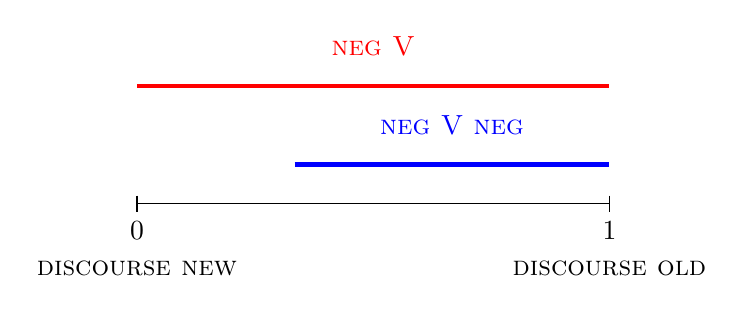
\begin{tikzpicture}
% \node (left) at (-1, 2)    {\includegraphics[width=.15\textwidth]{left.jpg}};
% \node (left) at (7, 2)    {\includegraphics[width=.15\textwidth]{right.jpg}};
%draw horizontal line
\draw (0,0) -- (6,0);
%draw ticks
\draw (0,3pt) -- (0,-3pt);
\draw (6,3pt) -- (6,-3pt);
%draw tick labels
\draw (0,0) node[below=3pt] {0} ;
\draw (6,0) node[below=3pt] {1} ;
\draw (0,-.5) node[below=3pt] {\textsc{discourse new} } ;
\draw (6,-.5) node[below=3pt] {\textsc{discourse old} } ;
%
\draw [ultra thick,red] (0,1.5) to (6,1.5);
\draw [ultra thick,blue] (2,.5) to (6,.5);
\draw (3,2) node {\textsc{\color{red} neg V}};
\draw (4,1) node {\textsc{\color{blue} neg V neg}};
% \draw (2,.25) node {$a_{\text{\textsc{\color{red} neg V}}}$};
% \draw (5,.25) node {$a_{\textsc{\color{blue} neg V neg}}$};

\end{tikzpicture}     
\end{center}
  \caption{Forms of negation given degree of inferrability}
  \label{continuum}
\end{figure}



The continuous representation also offers us some insight into \emph{why} Jespersen's Cycle occurs. The reasoning is as follows. First, keeping track of what is actually part of the discourse is difficult. In fact, this is the problem of \emph{common knowledge}\footnote{In epistemic logic \emph{mutual knowledge} only requires that everyone know that $p$, without any further steps. Thus anything that is common knowledge is also mutual knowledge, but not \emph{vice versa}. \cite{lewis:1969} introduced common knowledge in Philosophy. \cite{clark-marshall1981} use the term ``mutual knowledge'' to refer to common knowledge.}, that everyone knows that $p$, that everyone knows that everyone knows that $p$, \emph{ad infinitum}. \cite{clark-marshall1981} outline a set of reasonable heuristics for circumventing this infinite regress, including physical or linguistic co-presence and community membership. While these heuristics are made with reference to resolving the problem of common knowledge, they extend equally to 
propositions. Namely, propositions can be introduced to the discourse either explicitly (linguistic co-presence) or implicitly (physical co-presence, community membership).

Second, we have ample experimental evidence that speakers have particular biases in communication. Speakers tend to overestimate how successful they are at communication. \cite{savitsky-etal:2011} had two pairs of friends participate in a simple communication task. All four participants sat back to back and were individually given lists of four-way ambiguous sentences to read out loud with a specified meaning. For example, the sentence ``It's getting hot in here.'' could be interpreted as an indirect request to open the window or an amorous advance. Participants were asked to do two things. They were asked to guess the intended meaning of the sentences spoken by the other participants. They were also asked to estimate how many of the sentences the friend they came with had guessed correctly, and how many sentences the strangers from the other pair had guessed correctly. 

The results can be seen in Figure \ref{savitsky}. Listeners were reliably above chance at guessing the intended meaning out of the four potential meanings, but, friends and strangers did not differ significantly. However, speakers had much higher expectations  for listeners, significantly overestimating how many sentences listeners would accurately guess. This suggests that, as speakers, we often tend to overestimate how transparent our utterances actually are to our listeners.


\begin{figure}
\begin{center}
\includegraphics[width=.7\textwidth]{savitsky.pdf}          
\end{center}
  \caption{Results from \cite{savitsky-etal:2011}}
   \label{savitsky}
\end{figure}


\cite{lane-etal2006} offer evidence that is particular germane to the question of discourse status. The experimental design can be seen in Figure \ref{elephants-exp}. Participants were assigned the role of either the speaker or addressee in a communication game. Speakers were instructed to communicate information about a target shape to the addressee. One shape was visible to only the speaker, blocked from the view of the addressee by an occluder. In the target conditions, the item that was visible only to the speaker was the same shape, but varied along some relevant dimension (e.g. size, color). Figure \ref{elephants-results} shows the proportion of trials where speakers used a modifier in referring to the target item. Surprisingly, speakers' privileged information leaks into what is said. In fact, this happens to an even greater extent when speakers were explicitly instructed to conceal information about their privileged information.


\begin{figure}
\begin{center}
\includegraphics[width=.7\textwidth]{elephants-exp.png}          
\end{center}
  \caption{Experimental design of \cite{lane-etal2006}}
   \label{elephants-exp}
\end{figure}


\begin{figure}
\begin{center}
\includegraphics[width=.7\textwidth]{elephant-results.png}          
\end{center}
  \caption{Results for \cite{lane-etal2006}}
   \label{elephants-results}
\end{figure}

Returning to Jespersen's Cycle, we note that these experimental findings suggest a potential explanation for \emph{why} change takes place. The embracing form is restricted to a particular set of contexts where the proposition being negated is discourse old, or highly inferrable. If speakers tend to overestimate how inferrable the proposition being negated is, if they fail to filter out their own privileged information, then they will tend to use the embracing form in less and less inferrable contexts. The result will be an increase in the frequency of the embracing form over time. \cite{ahern-clark2015} offer a formal model of the dynamics of this process. However, the predictions of the model, like the corpus work by \cite{hansen2009, hansen-visconti2009}, are largely qualitative. That is, they demonstrate that the different forms of negation are sensitive to different constraints at different points in time, and offer an explanation of why those constraints might change over time. However, they offer no 
quantitative predictions about the shape of the change.

In contrast, \cite{wallage2013} presents a quantitative analysis of the conditioning factors of Jesepersen's Cycle in Middle English, drawing on evidence from the Penn Parsed Corpus of Middle English \citep{ppcme2}. Wallage codes sentences containing sentential negation for the discourse status of the proposition being negated, according to the categories outlined above. From two separate statistical tests on binned data (1150-1250 and 1250-1350), Wallage argues that if we factor out the overall rate of the embracing form, the effect of discourse status is not different across the two time bins. While the argument is interesting and it has great merit in being quantitative, the methodology is not compelling. That is, Wallage uses a form of \href{http://en.wikipedia.org/wiki/Variable_rules_analysis}{VARBRUL} and claims that the coefficients across discourse contexts are similar enough. There are several problems with this approach. First, it doesn't offer any way of quantitatively specifying how similar is 
similiar \emph{enough}. While regular practice may yield some insight, we want a statistical measure of how similar is similar enough to not reject the hypothesis that the conditioning of discourse status changes. Second, binning the data and not accounting for the potential effects of individual documents may yield misleading results. More appropriate methods, such as generalized linear mixed-effects models (GLMMs) would be more appropriate, and Wallage (p.c.) is moving towards the application of these new statistical techniques.

As it stands though, we don't have a clear answer to whether Jespersen's Cycle is driven by a sensitivity to discourse functional constraints. There are at least two potential explanations that reconcile the findings of \cite{hansen2009, hansen-visconti2009}, the experimental evidence of \cite{lane-etal2006}, the formal model of \cite{ahern-clark2015}, and the null result of \cite{wallage2013}. First, the role of discourse stats in Jespersen's Cycle may differ across languages. That is, the fact that the negation is sensitive to information structure may be particular to Romance languages. In fact, these constraints have only been noted in Romance languages. This could be the result of the constraints only occurring in Romance languages or just a lack of investigation into other languages synchronically and diachronically. The fact that the discourse status conditions in English don't change over time could be explained by this. However, it's striking that, at the beginning of the change, the embracing form 
in English is largely restricted to Inferrable and Discourse Old contexts. It would be surprising if this were a simple coincidence. Second, absent an explicit model of how and \emph{why} the discourse status constraints might be changing, the methodology employed by Wallage does not tell us much. That is, Wallage implicitly adopts the null hypothesis that the rate of change across discourse contexts is not different and argues that this null hypothesis cannot be rejected. However, it is not entirely clear what the null hypothesis ought to be, or if his method can actually tell us when we can reject it.

While we are still left with a fair amount of uncertainty regarding the actual causes of the cycle, it's clear that answering it will require a quantitative analysis of the conditioning factors of different forms of negation. The downside in this regard is that discourse status is not necessarily a surface property of sentences. That is, we cannot simply take a sentence and read off its relation to the previous discourse. Coding for discourse status requires a careful consideration of the prior context, the potential interpretations of a sentence, and general knowledge about the world.  This task is not straightforward even when analyzing contemporary language equipped with modern intuitions. The difficulty is only exacerbated when we turn to historical corpora. This leads to a reliance on expertise in the historical forms of a language to even perform a qualitative analysis, and a substantial investment of time and expertise to hand-code a large enough set of data to perform a quantitative statistical 
analysis. Unfortunately, this means that a comprehensive answer to the question of whether discourse constraints are important in Jespersen's Cycle is dependent on having experts in the history of multiple languages where the cycle has occurred invest a significant amount of time towards coding and evaluating the results. This is certainly possible, but also certainly a difficult task.

The goal of this project will be to explore methods for circumventing the need for significant expertise in the history of a language and significant time to understand the role of discourse status in change. In particular, we will be searching for surface properties of sentences that correlated with discourse status. On the assumption that these other surface properties stand in a stable relation to discourse status, we can probabilistically predict the discourse status of particular forms over time. That is, we are trying to infer the surface proxies of discourse status so that we can at least partially automate the process of determining the role of discourse in change. In the next section we describe the methods and data we will use.

\subsection{Signaling Game}

\subsection{Equilibria}

\subsection{Dynamics}

\subsection{Modeling}


%\section{Future Directions}
%
%This analysis suggests how Jespersen's Cycle can arise from signaling under a slight speaker bias. Examining the effect of these pragmatic pressures we established the following results. First, we showed that, for any amount of bias, emphatic forms become less informative over time. The extent of this loss is governed by the amount of bias, ranging from attenuation to complete bleaching. Second, only finitely many signals are stable in equilibrium for a given amount of bias.  The introduction of additional signals results in a push-chain scenario whereby the least informative signal is lost and the population returns to equilibrium. 
%
%There are several further directions that remain to be explored. First, we have encoded a bias on the part of the speaker into the utility function. This gives rise to the inflationary effect whereby emphatic negation is attenuated. However, it is not clear that this effect need arise from the speaker's preferences. For example, it may be the case that it could equally as well arise from the speaker's uncertainty regarding the hearers beliefs about the distribution over standards of precision. Thus far, we have relied on the \emph{common prior assumption}, which allows for the reduction of games of incomplete information to games of imperfect information \citep{harsanyi:1967,harsanyi:1968a,harsanyi:1968b}. That is, we have assumed that both speaker and hearer share the same prior probability over standards of precision. This need not be the case, but it is an open question as to whether removing this restriction yields a qualitatively different result than the course pursued here. Further, given every 
%individual's experience as both a sender and a hearer, the common prior assumption may be well justified.
%
%Second, we have assumed a uniform prior distribution over the state space. This serves well enough as a starting point, but the interaction between distributions and biases may yield dramatically different constraints than those discussed above. A straightforward generalization could be had by considering the \emph{Beta Distribution} over the state space, of which the uniform distribution is a special case. This would allow for a wide ranging test of the interaction between the prior probability and the amount of information that can be conveyed. Finally, the generalization of the prior can be informed in part by an empirical investigation of how often emphatic negation actually occurs. For example, if, as we have suggested, emphatic negation arises from NPIs in focus then we should be able to estimate the overall rate of use by determining how often such NPIs bear the mark of an abstract focus feature. That is, we can compare the overall rate of negation to the occurrence of NPIs with prosodic prominence.  
%While this only indirectly tells us about the underlying distribution of standards of precision, it provides a kind of constraint that will allow us to estimate likely distributions.


%%%%%%%%%
\part{The Formal Cycle}
% Learning Theory
\chapter{Stability}
\label{Stability}

\setlength{\epigraphwidth}{.9\textwidth}

\epigraph{It may be urged that change in language is due ultimately to the deviations of individuals from the rigid system. But it appears that even here individual variations are ineffective; whole groups of speakers must, for some reason unknown to us, coincide in a deviation, if it is to result in a linguistic change.\\ -- Leonard Bloomfield \citeyearpar[445]{bloomfield1927}}


%All this, de Saussure's la parole, lies beyond the power of our science. We cannot predict whether a certain person will speak at a given moment, or what he will say, or in what words and other linguistic forms he will say it. Our science can deal only with those features of language de Saussure's la langue, which are common to all the speakers of a community,?the phonemes, grammatical categories, lexicon, and so on. 

Distinguishing between the formal and functional Jespersen cycles simplifies the task of explanation. It allows us to disentangle two phenomena that overwhelmingly co-occur, and address them separately. For example, in the previous chapter we showed that the functional cycle in English can be explained in terms of the difficulty speakers have in keeping track of private versus common knowledge.  Crucially, this explanation of the transition from pre-verbal \emph{\textcolor{red}{ne}} to embracing \emph{\textcolor{blue}{ne...not}} rests on the way our pragmatic competence shapes the use and interpretation of linguistic signals over time. 

However, it is important to distinguish between the logical relationship between the two cycles and the explanation of a particular historical change. That is, the functional cycle can occur independently of the formal cycle, so we need an explanation for cases where it does occur independently. But, in the case of English, and many other languages, the functional cycle coincides with the first transition of the formal cycle. There is no guarantee that the model we described to address the functional cycle is the only or even the best explanation of the observed transitions of the formal cycle. That is, in any given case, pragmatic pressures might not explain the first transition of the formal cycle.

Here we consider other potential explanations for both of the transitions of the formal cycle.  In particular, we examine the possible role of acquisition. The facts to be explained are the transition from pre-verbal \emph{\textcolor{red}{ne}} to embracing \emph{\textcolor{blue}{ne...not}} and the transition from embracing \emph{\textcolor{blue}{ne...not}} to post-verbal \emph{\textcolor{green}{not}}. Our goal is to understand whether the process of acquisition offers any insights into why the formal cycle takes place. More broadly, we want to test whether grammatical competence and the process by which it is formed are sufficient to explain the observed changes.

First, we present a model of syntactic acquisition that has several desirable theoretical properties. Second, we determine the dynamics of the model in a population over time. In particular, we show the conditions under which the acquisition dynamics lead to change or stable variation. Third, we outline the syntactic structures at various stages of the formal cycle. These structures allow us to explicitly state the conditions for the acquisition dynamics to lead to either of the transitions of the formal cycle. Finally, we fit the model of the acquisition dynamics to data from the formal cycle in Middle English and discuss the implications of the fitted parameters.  

Acquisition can be taken as a cause of the formal cycle if only if the following qualitative and quantitative criteria are met. First, given the acquisition dynamics and grammatical structures underlying the formal cycle, we should predict the qualitative occurrence of both transitions. Second, if the acquisition dynamics predict the transitions, then the quantitative parameters of the dynamics fit to corpus data should be consistent with our theoretical assumptions. That is, the parameters of the model have some falsifiable empirical content that can be tested using corpus data. If neither of these criteria are met, then acquisition cannot explain the transitions of the formal cycle.

In fact, we show that neither of the transitions of the formal cycle observed in the history of English can be explained by acquisition. First, for the grammatical structures posited to underly the formal cycle the acquisition dynamics predict stability rather than change.  So, the first criterion cannot be met. Second, this also means that the second criterion cannot be met either; given that both transitions do occur, the parameters of the fitted model necessarily differ. In fact, it would seem that the only way acquisition could lead to either of the transitions would be, in Bloomfield's terms, a mass coincidence of deviation from the current system.

The main contributions of this chapter are twofold. First, we offer a general analysis of the acquisition dynamics, which clearly delineates the conditions for stability and change under certain kinds of parametric variation. Second, we make explicit the conditions for acquisition to play a role in either of the transitions of the formal cycle. In particular, one must show not only that acquisition predicts both transitions qualitatively, but that it also matches the quantitative trajectory of the change. It is important to note that these hold for any set of syntactic structures posited to underly the formal cycle. Demonstrating the role of acquisition requires demonstrating how the acquisition dynamics leads from one state to another.


\section{A model of acquisition}

In the most general sense, the process of language acquisition is some mapping from the initial state of the learner and the linguistic evidence provided to the learner to some terminal state, which is taken to be the grammatical competence of the speaker. We begin by introducing a model that can be used to describe this process. We then note some of the properties that make it an appealing model of acquisition.

The \emph{variational learning} model of acquisition \citep{yang2000internal,yang2002} consists of three basic components. First, there is a finite set of grammars that vary in a parametric fashion, in the sense of the  \emph{Principles and Parameters} framework \citep{chomsky1981,chomsky1995,chomsky-lasnik1993}. Second, a learner keeps track of a probability distribution over grammars, which we can think of as the weights of evidence the learner has for the various grammars. Third, a learner updates her distribution over grammars according to a learning scheme as she receives input from the linguistic environment.

To see this in detail, suppose that a learner is presented with sentences from the linguistic environment. The learner selects a grammar $G_i \in G = \{G_1,...,G_n \}$ with probability $p_i$ to analyze a sentence. There are two possible outcomes: either the grammar can analyze the sentence or it cannot. That is, the sentence is grammatical with respect to the selected grammar or it is not. The learner updates her distribution over grammars in the following manner, where $0 < \gamma \ll 1$ is a small learning parameter.


\begin{equation}
 \mbox{If $G_i \rightarrow s$ then }
\left\{
	\begin{array}{ll}
		p_i'  = (1 - \gamma)p_i + \gamma \\
		p_j'  = (1-\gamma)p_j & \mbox{for} j \neq i
	\end{array}
\right.
\end{equation}

\begin{equation}
 \mbox{If $G_i \nrightarrow s$ then }
\left\{
	\begin{array}{ll}
		p_i'  = (1-\gamma ) p_i \\
		p_j'  = (1-\gamma)p_j + \frac{\gamma}{n - 1} & \mbox{for} j \neq i
	\end{array}
\right.
\end{equation}
This is a \emph{linear reward-punishment} scheme \citep{bush-mosteller1955}:\footnote{This learning scheme is similar to the linear reward-inaction scheme that yields the replicator dynamics \citep{borgers-sarin1997}. It differs in that failures are not ignored, but rather punished. One compelling reason for treating learning differently across the domains of meaning and structure is the hypothesis space of each: the grammatical hypothesis space is heavily constrained, whereas the semantic hypothesis space, even under the Fodorian \citeyearpar{fodor1975} conception, is constrained but arguably unbounded. That is, even a finite set of innate concepts can be combined in the appropriate manner without end. Given this quantitative, if not qualitative difference between the domains, it is not clear how a learner would decide what aspects of a given hypothesized meaning to punish (cf. \citealt{quine1960}). But, see \cite{smith-yu2008,medina-etal2011,smith-etal2011, trueswell-etal2013} for experimental evidence, and \cite{yu-smith2007,frank-etal2009,stevens-etal2013} for computational approaches to the problem of learning meaning.} grammars that are compatible with a sentence drawn from the linguistic environment are rewarded, whereas grammars that are not compatible with the sentence are punished. Both of these actions are reflected in the first line of the two possible outcomes. If the grammar can analyze the sentence, then its probability is bumped up by some small amount determined by the learning parameter. If the grammar cannot analyze the sentence, then its probability is knocked down by some small amount determined by the learning parameter. The second conditions allow for the weights over grammars to be redistributed while guaranteeing that all probabilities always sum to one.

Now, the probability that a learner attributes to a grammar changes according to how successful that grammar is in dealing with the linguistic environment. In fact, the long term distribution over grammars can be determined from the probability that a grammar will not be able to analyze a sentence and will thus be penalized. For two grammars, $G_1$ and $G_2$, let the \emph{penalty probabilities} be $c_1$ and $c_2$, respectively. It can be shown that the expected value of the probabilities of the two grammars converge to the following limit values \citep[111]{narendra2012}.
\begin{equation}
\begin{split}
\lim_{t \rightarrow \infty} E[p_1(t)] &= \frac{c_2}{c_1 + c_2 }\\
\lim_{t \rightarrow \infty} E[p_2(t)] &= \frac{c_1}{c_1 + c_2 }
\end{split}
\end{equation}
We should note that this result is about the expected behavior of an individual, rather than the actual behavior of that individual. So, while the expected value of the probabilities converges to these values, the actual probability in the mind of a given learner does not. As we will see below, the actual values in the mind of an individual are close to, but not necessarily equal to these values. This distinction has important implications for the dynamics of acquisition, which we return to in the next section. In particular, it requires us to make certain assumptions about the size of the population.

%Second, the expected value of the probability of a grammar in the limit is directly proportional to the penalty probability of that grammar. Importantly, this means that learners get the appropriate ordering of weights to evidence, which is a property we would arguably expect of any learning model.

%�\footnote{This property holds for an arbitrary number of grammars \citep[117]{narendra2012}.}

So, we know the expected behavior of a learner given the penalty probabilities of the grammars in question. We can determine the penalty probabilities in the following manner. First, suppose that the linguistic environment is composed of the output of two partially incompatible grammars. Let $\alpha_1$ be the proportion of sentences generated at random by the first grammar $G_1$ that the second grammar $G_2$ cannot analyze; likewise let $\alpha_2$ be the proportion of sentences generated at random by the second grammar $G_2$ that the first grammar $G_1$ cannot analyze. Note that while the assumptions underlying them are theoretical both $\alpha_1$ and $\alpha_2$ empirical estimates of both can be calculated from a corpus (e.g. \citealt[94-95]{ingason-etal2013}).  We can represent the relationship between the two grammars visually as in Figure \ref{grammars-evidence} where the overlap of the two grammars indicate the sentences that are jointly analyzable by both grammars.  Second, let the linguistic environment be composed of some distribution over the two grammars, call it $L = p_1G_1 + p_2G_2$.  From this we can calculate the penalty probabilities as $c_1 = p_2\alpha_2$ and $c_2 = p_1\alpha_1$. The likelihood that the first grammar will not be able to analyze a sentence depends on the prevalence of the second grammar in the environment and the likelihood a sentence generated by that second grammar will be incompatible with the first grammar. The same reasoning holds for the second grammar. 

%That is, the likelihood that each of the grammars will not be able to analyze a sentence depends on the independent evidence for the other grammar and its prevalence in the environment.


\begin{figure}
\begin{center}
        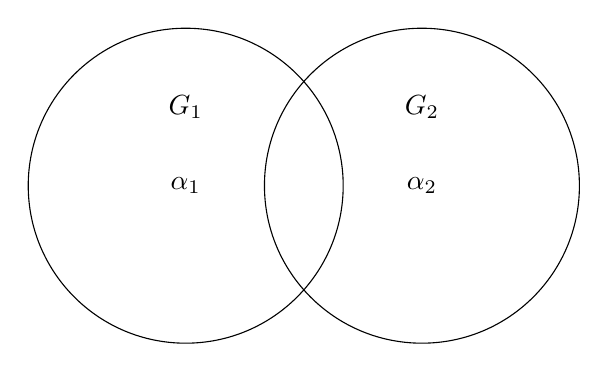
\begin{tikzpicture}
	  \node (A) [draw,circle,minimum size=4cm]  at (0,0) {$\alpha_1$};
	  \node (G1) [above of=A] {$G_1$};
	  \node [draw,circle,minimum size=4cm] (B) at (0:3cm) {$\alpha_2$};
	  \node (G2) [above of=B] {$G_2$};
	\end{tikzpicture}         
    \end{center}
\caption{Two partially incompatible grammars}
\label{grammars-evidence}
\end{figure}

We can get a sense for the learning process by simulating individual trajectories. This can be seen in Figure \ref{lrp-learning} where the horizontal axis represents time as additional sentences drawn from the environment and presented to the learner. The vertical axis represents the weight of $G_2$ in the learner's mind. We can compare the expected motion averaged across several hundred individual trajectories in bold to several individual trajectories. Where the expected motion smoothly approaches the value predicted by the model, shown by the dotted line, individual trajectories continue to move around the value. Again, we return to this important distinction in the next section when we turn to the dynamics of the model.

\begin{figure}
\begin{center}
	\includegraphics[width=.75\textwidth]{lrp-learning.png}\\
\end{center}
	\caption{Probability of $G_2$ over time for various individual trajectories and expected motion of trajectories, where $L=\frac{1}{2}G_1 + \frac{1}{2}G_2$,  $\alpha_1 = .1, \alpha_2 = .5, \gamma=.1$}
	\label{lrp-learning}
\end{figure}

However, before doing so, there are several important properties that are evident from the simulations presented in Figure \ref{lrp-learning}.  First, this learning model allows for the gradual adjustment of learners to the linguistic environment rather than abrupt changes (cf. \citealt{gibson-wexler1994,hyams-wexler1993}). Second, it allows learners to converge to distributions over grammars, rather than a single grammar \citep{kroch1989}. Third, the expected value of the probability of a grammar is directly proportional to its penalty probability  \citep[117]{narendra2012}, which means that learning is reasonably robust. These properties, along with the overall simplicity of the model make it an appealing starting point for investigating how acquisition might lead to change over time.


\section{The dynamics of acquisition}

We showed the properties of the variational learning model at the level of the individual; we now turn to the dynamics of learning in a population over time. First, we show how the expected change from one point in time to the next gives rise to a particular dynamics under particular assumption. Second, we show that the stable rest points of the dynamics are single grammars, with an important exception. We also show how these dynamics are closely related to the logistic model often taken as a proxy for changes in competing grammars.

Under the variational model, for the case of two grammars, we denote the expected value of the weight accorded to the grammar $G_2$ by a learner to be the following. That is, the average behavior of a learner converges to a probability determined by penalty probabilities and the prevalence of the two grammars in the linguistic environment.

\begin{equation}
p_2' = \frac{p_2 \alpha_2}{p_1 \alpha_1 + p_2 \alpha_2}
\end{equation}
Now, suppose that this distribution in turn serves as the linguistic environment for the next generation of learners. We can determine the expected change in the average weight of $p_2$ from one generation of learners to the next as the following.

\begin{equation}
\dot{p}_2 = p_2' - p_2 = \frac{p_2 \alpha_2}{p_1 \alpha_1 + p_2 \alpha_2} - p_2 = p_2(1-p_2)\frac{\alpha_2 - \alpha_1}{p_1 \alpha_1 + p_2 \alpha_2}
\end{equation}
This \emph{mean dynamics} follows the expected motion of the distribution over grammars in the population. Note that we are talking about the change in the expected behavior in the population. This means that we are modeling a fact about the population as a whole, which ultimately derives from individual learning. However, justifying the mean dynamics requires two important assumptions about the population.

The first assumption that must be made is about the size of the population. As we noted in the previous section, learners converge to the limit values only in expectation. In fact, an individual learner is almost always either slightly above or slightly below this expected value, as can be seen in Figure \ref{lrp-learning}. But, the distribution over these values in a population of learners at a given point in time is roughly normally-distributed around the limit value, as can be seen in Figure \ref{lrp-dist}. In this case, the expected value in the population is close to the limit value. As the population grows, the expected value in the population gets closer and closer to the limit value. In the limit of an infinite population, the linguistic environment for the next generation of learners is the limit value.\footnote{This is often a necessary assumption for studying the mean dynamics of what is undoubtedly a stochastic process. See Chapter 10 of \cite{sandholm2010} for a detailed derivation of the mean dynamics as the limit of a stochastic process in infinite population.    In the next chapter we relax the assumption of an infinite population, allowing for stochasticity in the change in the population over time.}
\begin{figure}
\begin{center}
	\includegraphics[width=.75\textwidth]{lrp-dist.png}\\
\end{center}
	\caption{Distribution over $p_2$ for population of learners and fitted normal distribution}
	\label{lrp-dist}
\end{figure}

The second assumption that must be made is about the structure of the population. Namely, the continuous-time form of the dynamics requires that we assume that there are continuously overlapping generations of learners that contribute to the linguistic environment.\footnote{A discrete-time dynamics might be more appropriate in allowing for a lag between when learners converge on a grammar and contribute to the linguistic environment, but this  distinction does not affect the subsequent results.} Together these assumptions guarantee that the dynamics track the expected weights over the grammars in the minds of learners over time. Thus, the solutions to this \emph{mean dynamics} is a model of the expected behavior in the population.

For the case of two grammars, we can simplify the dynamics in the following manner. Let $s = \frac{\alpha_2 - \alpha_1}{\alpha_2}$ and $p_2 = p$, then we have the following. In population genetics $s$ is referred to as the \emph{selection coefficient} of $\alpha_1$. For cases where $s > 0$,  $\alpha_2 $ has a selective advantage and $\alpha_1$ is selected against. For $s=0$, $\alpha_1$ and $\alpha_2$ are selectively \emph{neutral}.

\begin{equation}
\dot{p} = p(1-p)\frac{s}{1- s(1-p)}
\end{equation}
We can read the rest points off the resulting acquisition dynamics. There are two important cases that we will consider. First, if there is only a single grammar, then the weight over grammars is stable. That is, if $p=0$ or $p=1$, then the dynamics are, so to speak, at rest.  This makes intuitive sense, a grammar cannot be considered if there is no evidence for it. Second, if there is a perfectly balanced amount of independent evidence for both grammars $s = 0$, then any distribution over grammars is a rest point. This also makes intuitive sense, if the balance of evidence is equally in favor of both grammars, then things should not change. We determine the stability of these sets of rest points in turn.

For the first set of rest points, we can evaluate the stability of a single grammar as a function of the selection coefficient, which captures the ratio of independent evidence in favor of one or the other grammar. To do so we evaluate the derivative of the dynamics at the two rest points constituted by a single grammar. If the derivative evaluated at the rest point is negative, then the rest point is \emph{asymptotically stable}. That is, the dynamics will carry the population to the rest point. If the derivative evaluated at the rest point is positive, then the rest point is \emph{unstable}. That is, the dynamics will carry the population away from the rest point. We can express these conditions as a function of the selection coefficient, $s$. 

\begin{equation}
\frac{\partial \dot{p}}{\partial p} \big|_{p=0} = \frac{s}{1-s}
\end{equation}

\begin{equation}
\frac{\partial \dot{p}}{\partial p} \big|_{p=1} = -s
\end{equation}
Note that for $s \neq 0$, only one of these rest points can be asymptotically stable. The rest point $p=0$ is asymptotically stable if and only if $s < 0$. That is, the population will eventually use grammar $G_1$ exclusively if only if there is more evidence for it than there is $G_2$. The rest point $p=1$ is stable if and only if $s > 0$. That is, the population will eventually use grammar $G_2$ exclusively if and only if there is more evidence in favor of it. 

In fact, these conditions for the stability of both rest points are rather general. If we assume that the selection coefficient is not zero, then there are no other rest points. So, these conditions amount to conditions for \emph{global asymptotic stability}. Importantly, this means that no matter the initial distribution over grammars, if $s > 0$ then grammar $G_2$ will take over in the population. Thus, the acquisition dynamics are a kind of frequency-independent selection. We can get a sense for this fact by visualizing trajectories from the same low starting state of $p$ for various values of $s$ as in Figure \ref{lrp-gain}. No matter how small the initial proportion or slim the margin of evidence, it is guaranteed to eventually go to completion. 

%Under these dynamics, acquisition is a particularly robust process over time.

%\footnote{\citet[239]{yang2000internal} refers to this as the \emph{fundamental theorem of language change}.}

\begin{figure}
\begin{center}
 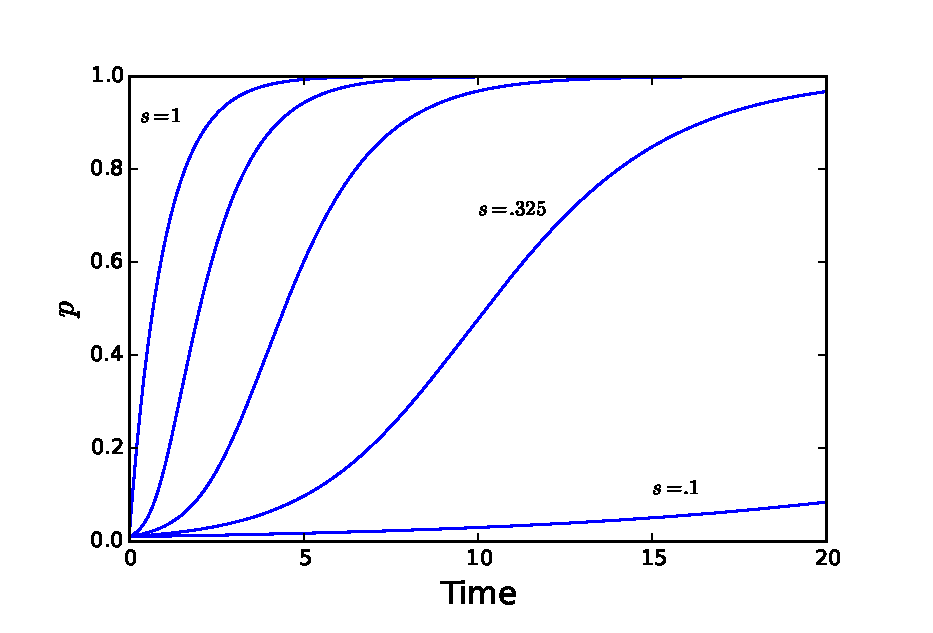
\includegraphics[width=.75\textwidth]{lrp-gain.eps}\\
\end{center}
	\caption{Proportion of $G_2$ over time for various ratios of evidence $s > 0$}
	\label{lrp-gain}
\end{figure}


Interestingly, the acquisition dynamics in these cases are closely related to the logistic models originally posited by \cite{altmann-etal1983} and \cite{kroch1989} to underly competing grammars. While there was no specific learning mechanism underlying the logistic model, it has both connections with the notion of biological competition as well as a straightforward application in terms of logistic regression (cf. \citealt[4]{kroch1989}). However, it is obvious that the variational model provides some justification for this conception when we compare the dynamics of logistic growth with the acquisition dynamics, where $s$ is taken as the growth rate in the logistic model.

\begin{equation}
	\dot{p} = p(1-p)s
\end{equation}
In fact, the only difference is that the acquisition dynamics exhibits a varying growth rate as a function of the distribution over grammars in the population. We show the solution for the acquisition dynamics and the logistic model from the same starting point with the same growth rate in Figure \ref{lrp-log}. The solution to the acquisition dynamics predicts a faster initial rate of growth, but slows down to the same rate as the logistic as $p \approx 1$.

\begin{figure}
\begin{center}
 \includegraphics[width=.75\textwidth]{lrp-log.png}\\
\end{center}
	\caption{Solution to acquisition dynamics and logistic model (dashed) from same starting point with $s=.4$}
	\label{lrp-log}
\end{figure}


In many cases the predictions of the two underlying models may not be distinguishable. But, it is certainly possible that we might detect quantitative evidence for the acquisition dynamics. For example for selection coefficients $s \approx 1$ the acquisition dynamics are asymmetric, unlike the logistic, which is perfectly symmetric. This can be seen in the first few solutions in Figure \ref{lrp-gain}. In the context of regression this could potentially lead to quantitative patterns such as heteroscedastic residuals. For example, if we take the acquisition dynamics as a generative model, then fit of the logistic model may systematically under or overestimate the rate of change at different points. We leave investigating this possibility for future research. 

For the second set of rest points, where both grammars have equal independent evidence $s=0$, all distributions over grammars are rest points. All states are \emph{weakly} or \emph{lyupanov stable} in the sense that though the dynamics do not carry the population to a state, the also do not carry the population away from it. Now, we might wonder whether these seemingly knife-edge cases are likely if even possible. However, these cases have a natural interpretation and one that will be particular relevant to the formal cycle. That is, they describe cases where the difference between two grammars hinges on the expression of a single syntactic position. If two grammars correspond to two ways of expressing that position, then the output of each will be incompatible with the other. That is, they will be totally mutually incompatible grammars, rather than only partially incompatible grammars. This can be visualized as in Figure \ref{grammars-incompatible}, which stands in contrast with Figure \ref{grammars-evidence}. In other words, where two grammars vary parametrically at the appropriate level, the dynamics predict a kind of weak stability.

\begin{figure}
\begin{center}
        \begin{tikzpicture}
	  \node (A) [draw,circle,minimum size=4cm]  at (0,0) {$\alpha_1$};
	  \node (G1) [above of=A] {$G_1$};
	  \node [draw,circle,minimum size=4cm] (B) at (0:5cm) {$\alpha_2$};
	  \node (G2) [above of=B] {$G_2$};
	\end{tikzpicture}         
    \end{center}
\caption{Two totally incompatible grammars}
\label{grammars-incompatible}
\end{figure}


So, we determined the acquisition dynamics resulting from the variational model and showed how it exhibits a kind of frequency-independent selection. That is, in most cases only a single grammar is stable. We showed how the resulting dynamics resembles the logistic model of growth. We also noted a crucial exception to this rather robust behavior that leads to a weak kind of stability.  With this in mind, we now turn to an analysis of the syntactic structures underlying the formal cycle.

\section{The syntactic structures of the formal cycle}

There are a range of ways of analyzing the syntactic structures underlying the formal cycle.\footnote{For example, different analyses have suggested varying levels of detail in the number and realization of stages, ranging from three stages  \citep{burridge1983,bernini-ramat1996,haspelmath1997,frisch1997,zanuttini1997,horn:1989,hoeksma1997,horn2001,roberts-roussou2003,vanderAuwera-neuckermans2004,mazzon2004,willis2005,lucas2007,jager2008,wallage2008}, to four stages \citep{dahl:1979,schwegler1988,schwegler1990,schwenter2005,schwenter2006}, up to five stages \citep{honda2000,beukema1999,vanderAuwera-neuckermans2004,zeijlstra2004}.} Here we focus on the analysis presented in \cite{frisch1997}, which treats the formal cycle as the result of two independent morphological changes. First, we present the theoretical details of the analysis. We then note corpus evidence in favor of this treatment.

% Finally, we explicitly state the grammars posited to underly the formal cycle.


\cite{frisch1997} takes Pollock's \citeyearpar{pollock1989} analysis of  negation as a starting point, assuming that negation constitutes its own phrase, with a fully projected structure like that in Figure \ref{negp}: Neg$^0$ is the head of the phrase, Spec is its specifier, and XP is a sister phrase such as a verb phrase.  In particular, Frisch assumes that this underlying structure is always present  \citep{haegeman1995}. The formal cycle simply consists in changes to how the positions in this underlying structure are expressed.\footnote{This is a more localized version of the  \emph{cartographic approach} advocated by \cite{rizzi1997}, which posits a universal syntactic structure. The locus of variation between languages under this conception is how that universal structure is expressed.}


\begin{figure}
        \Tree [.NegP [. Spec ]
        [.Neg$'$ Neg$^0$
        XP ] ]

\caption{The structure of the Negative Phrase} 
\label{negp}
\end{figure}

%However, he treats the embracing form as epiphenomenal, arising from two independent morphological changes in a fixed underlying structure. The assumption of a fixed structure can be stated as in Haegeman's \citeyearpar{haegeman1995} \emph{Neg-criterion} on negative phrases.
%
%\begin{definition}
%The Neg-criterion
%\begin{enumerate}
%	\item Each Neg $X^0$ must be in a spec-head relationship with a Neg operator.
%	\item Each Neg operator must be in a spec-head relationship with a Neg $X^0$.
%	\item Neg-operator: a NEG phrase in a scope position
%	\item Scope position: a left-peripheral A -position (i.e. XP-adjoined or Spec).
%\end{enumerate}
%\end{definition}

%This criterion simply requires that the negative phrase always have the full structure as in Figure \ref{negp}, including a head and a specifier. The strongest form of this assumption posits a universal syntactic structure, where the locus of variation between languages lies in how this universal structure is expressed (cf. the \emph{cartographic} approach advocated by \citealt{rizzi1997}, \emph{inter alia}).

At the first stage of the formal cycle the negative head is expressed as \emph{ne} whereas the specifier is a phonologically null operator $\varnothing$. The syntactic structure according to this morphological analysis can be seen in Figure \ref{stage1morphology}. Sentential structure at stage one of the formal cycle in Old English is illustrated in Figure \ref{sentence1morphology}, where a strikethrough indicates successively upwards head movement. The result is purely pre-verbal negation.

%$_{[+\text{NEG}]}$
\begin{figure}
        \Tree [.NegP [.XP $\varnothing$ ]
        [.Neg$'$ [.Neg \emph{ne}
        ] [.VP \edge[roof]; {...} ] ] ]

\caption{Stage one of the formal cycle according to morphological analysis}
\label{stage1morphology}        
\end{figure}


\begin{figure}
        \Tree [.TP [.DP ic ] [.T$'$ [.V+Neg+T {ne secge} ] [.NegP $\varnothing$
        [.Neg$'$ [.\sout{V+Neg}
        ] [.VP \sout{V} ... ] ] ] ] ]

\caption{Sentential structure at stage one of the formal cycle according to morphological analysis}
\label{sentence1morphology}
\end{figure}

The transition to the second stage in the formal cycle stems from a change in the realization of the specifier of the negative phrase. Namely, the specifier is no longer expressed by a null operator, but instead by \emph{not}, as can be seen in Figure \ref{stage2morphology}. Sentential structure at the second stage of the formal cycle in Middle English is illustrated in Figure \ref{sentence2morphology}, which results in pre- and post-verbal negative elements.


\begin{figure}
        \Tree [.NegP [.XP \emph{not} ]
        [.Neg$'$ [.Neg \emph{ne}
        ] [.VP \edge[roof]; {...} ] ] ]

\caption{Stage two of the formal cycle according to morphological analysis}
\label{stage2morphology}        
\end{figure}


\begin{figure}
        \Tree [.TP [.DP I ] [.T$'$ [.V+Neg+T {ne seye} ] [.NegP \emph{not}
        [.Neg$'$ [.\sout{V+Neg}
        ] [.VP \sout{V} ... ] ] ] ] ]

\caption{Sentential structure at stage two of the formal cycle according to morphological analysis}
\label{sentence2morphology}
\end{figure}

%At this point in the formal cycle we might wonder whether the introduction of two negative elements is problematic. That is, if each element contributes semantic negation in its own right, then the two might cancel each other out. In classical terms, a doubly negated proposition is logically equivalent to the bare proposition.  To circumvent this problem \cite{frisch1997} argues for the \emph{Economy of Projection} principle posited independently by \cite{speas1994}.

%\footnote{Of course, this equivalence ceases to hold in intuitionistic logic, which abandons the elimination of double negation $\neg \neg p \leftrightarrow p$ and the law of the excluded middle $p \vee \neg p$ in favor of a proof-theoretic approach.}

%\begin{definition}
%Economy of Projection principle
%\begin{enumerate}
%	\item Project a phrase XP only if XP has content
%\end{enumerate}
%\end{definition}

%This principle simply states that we can only posit syntactic structure where we have some evidence for it. In this case, the negative phrase is licensed if it contains material in either the head or the specifier. In other words, neither element is necessary for the phrase to occur, so neither can be responsible for the contribution of negative meaning by itself. Rather, it is the negative phrase as a whole that contributes semantic content of negation to the sentence. This can be seen in Figures \ref{stage1morphology} and \ref{stage2morphology} where it is the entire negative phrase that carries the $[+\text{NEG}]$ feature of semantic negation.

The transition from the second stage to the third and final stage of the formal cycle is simply a a matter of whether the negative head is expressed via lexical content or by some null head $\varnothing$. The structure of the negative phrase at the third stage is shown in Figure \ref{stage3morphology}, and sentential structure at this final stage in Late Middle English is shown in Figure \ref{sentence3morphology}. 

%Subsequent stages of negation can be derived by considering the loss of verb raising and the rise of \emph{do}-support.

\begin{figure}
        \Tree [.NegP [.XP \emph{not} ]
        [.Neg$'$ [.Neg $\varnothing$ ]
        [.VP \edge[roof]; {...} ] ] ] 

\caption{Stage three of the formal cycle according to morphological analysis}
\label{stage3morphology}
\end{figure}

\begin{figure}
        \Tree [.TP [.DP I ] [.T$'$ [.V+Neg+T {say} ] [.NegP \emph{not}
        [.Neg$'$ [.\sout{V+Neg}
        ] [.VP \sout{V} ... ] ] ] ] ]

\caption{Sentential structure at stage three of the formal cycle according to morphological analysis}
\label{sentence3morphology}
\end{figure}

Similar morphological approaches to the formal cycle are adopted by \cite{roberts-roussou2003} and \cite{zeijlstra2004}. The shared aspect of these morphological analyses is the assumption that the underlying syntactic structure remains stable, but the realizations of particular positions within that structure changes. Importantly, since this is the only locus of change, the transitions that constitute the cycle are independent of each other. That is, the fact that both \emph{ne} and \emph{not} show up in the embracing \emph{\textcolor{blue}{ne...not}} form is simply the coincidental product of two forms waxing and waning at the same time.

\cite{frisch1997} tests this theoretical prediction using the trajectory of negation in Middle English in the Helsinki corpus of Middle English. He notes that if the two transitions are independent of each other, then the co-occurrence of \emph{ne} and \emph{not} in the negative phrase should be the product of the probabilities of each occurring. 

\begin{equation}
	P(\emph{\textcolor{blue}{ne...not}}) = P(\emph{ne})P(\emph{not})
\end{equation}
That is, the probability of \emph{\textcolor{blue}{ne...not}} is the probability of two independent events \emph{ne} and \emph{not}. This is in fact what Frisch finds.\footnote{Calculating these probabilities requires some adjustment for things like instances of adverbial \emph{not} among others. See \citet[32-47]{frisch1997} for the details.} So the formal cycle can be conceived of as two changes in the expression of positions within an underlying structure. In what follows, we will assume that grammatical knowledge is represented as in Figures \ref{stage1morphology}, \ref{stage2morphology}, and \ref{stage3morphology}. That is, under the assumption of a constant underlying structure, a grammar is characterized by the mapping from the syntactic positions in the negative phrase to lexical items. With these definitions in place, we turn to the actual trajectories of the transitions of the formal cycle in English.


%Frisch estimates the probabilities required to test this prediction in the following manner. First, he estimates the total tokens of \emph{ne} by simply counting the appearances of \emph{ne}. Second, the number of relevant \emph{not} tokens has to be adjusted to exclude adverbial tokens of \emph{not}, which are not part of the negative phrase. Frisch uses the distribution of the adverbial \emph{never} pre- and post-verbally to estimate the proportion of adverbil \emph{not}. Namely, if adverbial \emph{not} is distributed in similar proportions pre- and post-verbally, then the total number of adverbial \emph{not} tokens can be estimated from the total number of pre-verbal tokens. With this adjustment, the probability of both \emph{ne} and \emph{not} can be calculated and compared to their joint probability. Treating the embracing form in this manner yields a good fit to the data.

%\footnote{See \cite[52]{frisch1997} Table 13 for details of the $\chi ^2$ test results. See Tables 9, 10, and 11 for the construction of Table 13.}

%If the appearance of \emph{ne} and \emph{not} together as \emph{\textcolor{blue}{ne...not}} is simply coincidental, then how are we to characterize the grammatical knowledge underlying the different stages of the formal cycle? I


%So, the grammar at the first stage of the formal cycle maps the head of the negative phrase to \emph{ne} and the specifier to a null operator $\varnothing$, the grammar at the second stage of the formal cycle maps the head to \emph{ne} and the specifier to \emph{not}, and the grammar at the third stage of the formal cycle maps the head to a null element $\varnothing$ and the specifier to \emph{not}.

%\begin{equation}
% \mbox{$G_1 : $}
%\left\{
%	\begin{array}{ll}
%		Neg^0 \rightarrow ne\\
%		Spec \rightarrow \varnothing
%	\end{array}
%\right.
%\end{equation}
%
%\begin{equation}
% \mbox{$G_2 : $}
%\left\{
%	\begin{array}{ll}
%		Neg^0 \rightarrow ne\\
%		Spec \rightarrow not
%	\end{array}
%\right.
%\end{equation}
%
%\begin{equation}
% \mbox{$G_3 : $}
%\left\{
%	\begin{array}{ll}
%		Neg^0 \rightarrow \varnothing \\
%		Spec \rightarrow not
%	\end{array}
%\right.
%\end{equation}
%With these definitions in place, we turn to the actual trajectories of the transitions of the formal cycle in English.

%\footnote{\citet[56]{frisch1997} explicitly assumes that the formal cycle is simply a transition from one method of licensing the negative phrase to another, and ``does not necessitate invoking two underlying grammars (\emph{I-languages} in the sense of \cite{chomsky1986}), as the old and new systems do not vary on a particular parameter." This is, perhaps, a strange characterization insofar as the first and last stages do indeed vary parametrically with regard to whether the head and specifier of the negative phrase are expressed by non-null elements.}


%At the heart of this question is the amount of evidence that a given element expresses negation. At the beginning of the change clearly only the preverbal negator does so. The postverbal reinforcer only emphasizes this negation. Eventually though, the evidence weighs in favor of the postverbal negator alone being the expression of negation. \cite{wallage2008} characterizes this transition in morphosyntactic terms as the loss of a [+NEG] feature on the preverbal negator, along with the concomitant introduction of a [+NEG] feature on the postverbal negator. This then allows for the loss of the preverbal negator given that the negative feature can be found elsewhere in the sentence.


%We can formulate the effect of various amounts of evidence in terms of Yang's \citeyearpar{yang2002} variational model. First, let there be two grammars, $G_{ne}$ and $G_{not}$, that represent the location of the abstract feature at \emph{ne} and \emph{not} respectively. We can represent the relation between the two grammars schematically as in Figure \ref{grammars}. In this case, $\alpha$ indicates the proportion of the linguistic environment that is only compatible with $G_{ne}$, and $\beta$ indicates the portion of the linguistic environment that is only compatible with $G_{not}$. The proportion of the two grammars in the population is governed by the following learning rule, where $p_0$ and $p_t$ represent the proportion of $G_{ne}$ in the population after $0$ and $t$ generations, and $q_0$ and $q_t$ represent the proportion of $G_{not}$ after $0$ and $t$ generations.


\section{Modeling the formal cycle}

%Now a problem of parameter interference immediately arises. Under the parametric representation of grammars, grammar selection is based on independent parameters. By contrast, fitness measure and thus the outcome of learning�reward or punish- ment�is defined on whole grammars.

Now that we have stated the grammars underlying the stages of the formal cycle we can turn to modeling the transitions of the formal cycle. First, we note that given the structure of the grammars posited to underly the formal cycle, we can treat each of the transitions separately. Second, we note that given the composition of the grammars we should expected stability under the acquisition dynamics. Finally, we fit the acquisition model for the two transitions of the formal cycle and note that the parameters are indeed not what the acquisitions dynamics predict. However, we note what a successful explanation of the formal cycle would have to do.

The grammars underlying the formal cycle differ only in the expression of two syntactic positions. This has two important implications. First, if the two changes in how these positions are expressed are independent of each other, then we can treat them as such. That is, we can treat the two transitions of the formal cycle as independent events of competition between two grammars for expressing those positions. In what follows we take this approach, treating both the first and second transitions as cases of the acquisition dynamics with two grammars. Second, if the grammars involved in each transition differ only in the expression of one position, then they are totally mutually incompatible $s=0$. This means that the acquisition dynamics predict stability in the case of both transitions, but this is certainly not what we observe. In fact, this alone suffices as a demonstration that acquisition as we have modeled it here cannot account for either of the transitions of the formal cycle.  That is, given the description of the grammars underlying the stages of the formal cycle, acquisition cannot cause the transitions between them. This means that the qualitative criterion for acquisition serving as a cause of the formal cycle is not met.

However, it is useful to note what would have to be the case for acquisition to explain the empirical trajectories of the two transitions. That is, if we fit the acquisition dynamics to data, the fitted parameters tell us what we would need to find in order to take acquisition as the cause of the formal cycle. We fit the acquisition dynamics to the trajectory of the first transition modeled as the competition of two grammars for the specifier of the negative phrase. In this case we take $G_1$ as $G_\varnothing$ and $G_2$ as $G_{not}$ to be grammars that determine how the specifier of the negative phrase is expressed.  We take instances of \emph{\textcolor{red}{ne}} to be compatible with $G_\varnothing$ and instances of \emph{\textcolor{blue}{ne...not}} and  \emph{\textcolor{green}{not}} to be compatible with $G_{not}$. The parameters to fit are the initial state of the second grammar in the population and the selection coefficient  $s$ that captures the ratio of evidence in favor of the second grammar. 

The last thing that needs to be specified is the notion of time. The solution to the acquisition dynamics is in abstract time units, but how these correspond to the actual time in days, months, or years is unspecified. We could fit this relationship as another parameter in the model, but this would be problematic if we were to find different values for the second transition. Instead, we stipulate a ratio between the units of the dynamics and years where one abstract time unit corresponds to five years. We take this to be a rough approximation of the time between when a learner is born an starts contributing to the linguistic environment, but leave it to further research to gain a better estimate the actual value.

The results of fitting the acquisition dynamics can be seen in Figure \ref{lrp-first}.\footnote{See Appendix C for details.} It is important to note, however, that regardless of how well the fitted model approximates the actual trajectory of the first transition, the parameters are not possible. That is, the second grammar cannot have an advantage over the first given that they differ only in the expression of a single syntactic position, yet this is exactly what would be required for acquisition to explain the first transition. This means that the quantitative criterion for acquisition serving as a cause of the formal cycle is not met. However, for another description of the grammars underlying the stages of the formal cycle, this parameter would need to match our theoretical predictions. That is, if the grammars were specified differently, the selection coefficient $\hat{s}$ would still have empirical content. We should be able to look at a corpus and use the grammatical descriptions to see if it is consistent.

\begin{figure}
\begin{center}
 \includegraphics[width=.75\textwidth]{lrp-first.eps}\\
\end{center}
	\caption{Proportion of $G_{not}$ over time for the first transition of the formal cycle, $\hat{s} = 0.10291529$}
	\label{lrp-first}
\end{figure}

We also fit the acquisition dynamics to the trajectory of the second transition modeled as the competition of two grammars for the head of the negative phrase. In this case we treat $G_1$ as $G_{ne}$ and $G_2$ as $G_\varnothing$.  We take instances of \emph{\textcolor{red}{ne}} and \emph{\textcolor{blue}{ne...not}} to be compatible with $G_{ne}$ and instances of \emph{\textcolor{green}{not}} to be compatible with $G_\varnothing$. The results of fitting the acquisition dynamics can be seen in Figure \ref{lrp-second}.\footnote{We only fit the dynamics to data from the point where there are instances of \emph{\textcolor{green}{not}} in all subsequent years, from 1300 CE onwards. Again, see Appendix C for details.} Again, this means that our second criterion for acquisition serving as a cause of the formal cycle is not met. So, neither of the criteria for acquisition serving as a cause of the formal cycle have been met. That is, the acquisition dynamics do not predict either of the transitions, nor do the parameters of the fitted models agree with the corpus evidence predicted by the grammars.

\begin{figure}
\begin{center}
 \includegraphics[width=.75\textwidth]{lrp-second.eps}\\
\end{center}
	\caption{Proportion of $G_\varnothing$ over time for the first transition of the formal cycle, $\hat{s} = 0.34128455$}
	\label{lrp-second}
\end{figure}


It bears emphasis that these criteria are not specific to the acquisition dynamics we specified nor to the grammatical structures posited to underly the stages of the formal cycle. We could just as well adopt another model of acquisition or the grammatical description of the formal cycle (cf. \citealt{niyogi2006}).  But, abandoning the appealing theoretical properties of the variational model and its acquisition dynamics seems a bit hasty. This is especially true given that we need some model to provide any explanation at all. There are, however, a wealth of options when it comes to grammatical descriptions of the formal cycle, as we noted above. 

For example, \cite{wallage2008} makes a compelling corpus-driven argument for the treatment of the formal cycle as two interdependent morphosyntactic changes. In particular, Wallage treats the first transition as the addition of the post-verbal \emph{not} as well as the change in the formal features of pre-verbal \emph{ne} from an interpretable to an uninterpretable feature \citep{chomsky1995}. This more articulated approach would likely face the same problem regarding the first transition, but might offer insight into the second transition. But, it would also offer an interesting alternative insofar as it takes the locus of variation to be the properties and features of functional categories, according to the so-called \emph{Chomsky-Borer conjecture}, \citep{baker2008}.

But, regardless, for acquisition to explain the formal cycle, both of the criteria we described above have to be met. Not only must both of the transitions be predicted, they must also be modeled in an empirically and theoretically consistent manner. To perhaps belabor the point, we can use the parameters of the fitted models of the transitions to predict the proportion of the different forms of the formal cycle in English over time. The result can be seen in Figure \ref{lrp-combined}, and indeed the predicted forms are a close match to the empirical trajectories that we observe. It is tempting to take this as a reasonably good result. But, the parameter values that generate this result are on their face not compatible with the grammatical structures posited to underly the formal cycle. If we want to explain, rather than just describe historical changes we need models that get the picture right while simultaneously being self-consistent. That is, we not only need to be able to fit parameters, but also to make sure those parameters make sense given our theoretical assumptions about the grammatical knowledge that speakers acquire.


\begin{figure}
\begin{center}
 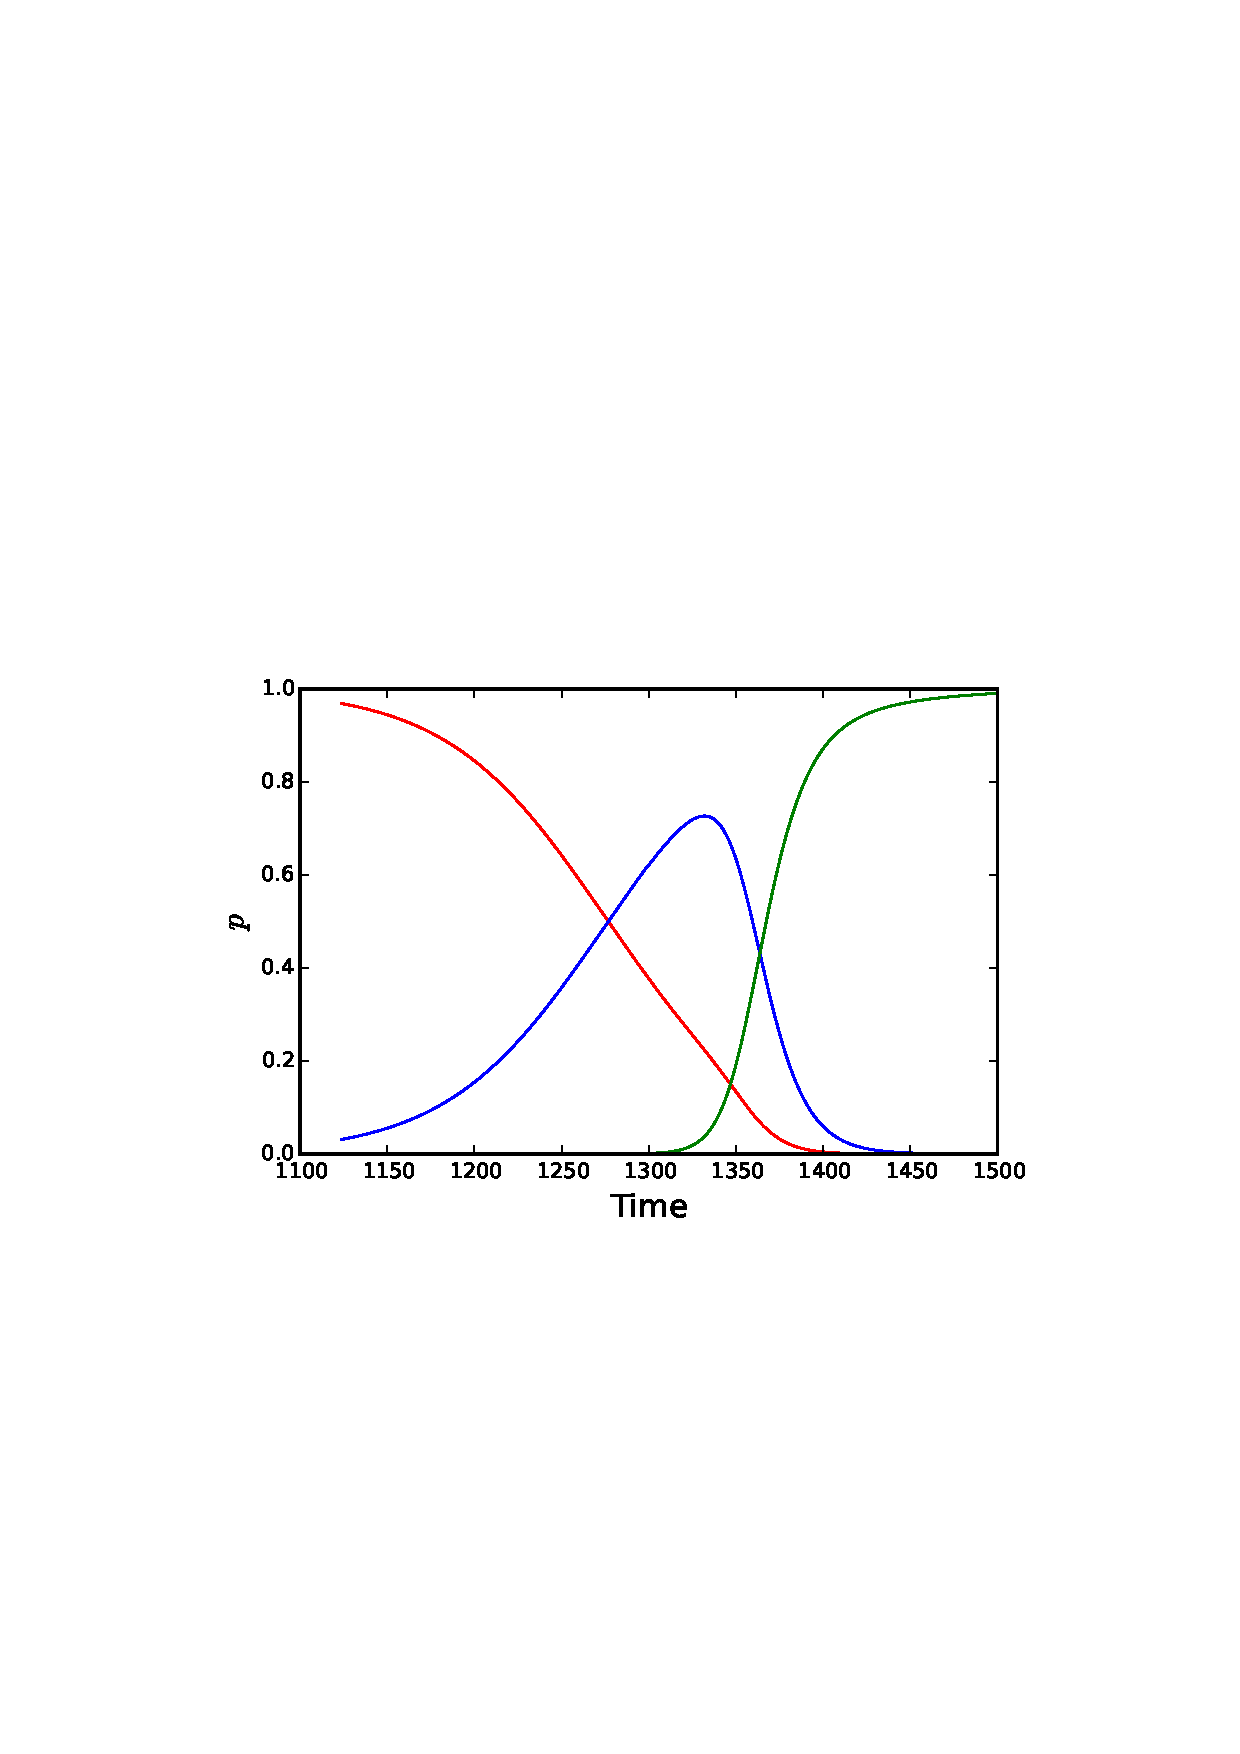
\includegraphics[width=.75\textwidth]{lrp-combined.pdf}\\
\end{center}
	\caption{Proportion of \emph{\textcolor{red}{ne}}, \emph{\textcolor{blue}{ne...not}}, and \emph{\textcolor{green}{not}} predicted by the fitted parameters of the acquisition dynamics}
	\label{lrp-combined}
\end{figure}


\section*{Summary}

In this chapter we presented a model of syntactic acquisition, determined its predicted dynamics in a population over time, and fitted it to data from the formal cycle in Middle English. We found that neither the qualitative nor quantitative criteria for taking acquisition as the cause of the formal cycle were met. All together then, it seems that acquisition cannot be taken as a cause of the formal cycle. If this is indeed the case, then it has important consequences for our understanding of the two transitions of the formal cycle.

Regarding the first transition from \emph{\textcolor{red}{ne}} to \emph{\textcolor{blue}{ne...not}}, if acquisition cannot explain it, then use can. That is, given that this transition coincides with the functional cycle, then the explanation of the functional cycle put forward in the previous chapter is the only and necessarily  the best explanation of the observed transition. Alternative analyses of the grammars underlying the formal cycle may change this, they must be both qualitatively and quantitatively accurate and consistent. 

Regarding the second transition from \emph{\textcolor{blue}{ne...not}} to \emph{\textcolor{green}{not}}, neither acquisition nor use can explain it. The transition does not coincide with another functional cycle, \emph{\textcolor{green}{not}} is not restricted to specific contexts.  This leaves us in the strange position of observing a change without an obvious cause.  Absent some mass coincidence, what are we to make of the second transition of the formal cycle? One possibility is that this second transition is not the result of one mass coincidence, but rather the accumulation of many much smaller coincidences.

To see how this might be the case, consider the fact that the acquisition dynamics only predict a weak form of stability in the expected change of the expected behavior of learners in a population. For example, if we relaxed the assumption regarding the size of the population, then the linguistic environment provided to learners would differ slightly from the limit value. For the second transition, suppose that the proportion of $G_\varnothing$ in the actual linguistic environment is slightly higher than expected due to sampling errors. Now, suppose that it is slightly higher in the next generation as well due to sampling errors. If enough of these small coincidences compound over time, one grammar may replace another without ever having more evidence in favor of it. 

Indeed, this possibility has been extensively studied in population genetics in terms of \emph{genetic drift}. That is, when the selection coefficient is zero $s=0$, as is the case in the second transition of the formal cycle, change can come about due to random sampling. Or, in this case, random changes in the probabilities over grammars learned over time. This means that we the second transition might be the result of a series of small coincidences rather than a single improbable one. In the next chapter we turn to means of testing this possibility.

% Stability
\chapter{Chance}
\label{chance}

\setlength{\epigraphwidth}{.9\textwidth}

\epigraph{[T]o my imagination it is far more satisfactory to look at such instincts as...consequences of one general law leading to the advancement of all organic beings -- namely, multiply, vary, let the strongest live and the weakest die.\\--Charles Darwin \citeyearpar{darwin1859}}

%\\ \hspace{12pt}
%
% God does not play dice with the world.\\--Albert Einstein}


%Finally, it may not be a logical deduction, but to my imagination it is far more satisfactory to look at such instincts as the young cuckoo ejecting its foster-brothers,�ants making slaves,�the larv� of ichneumonidea feeding within the live bodies of caterpillars,�not as specially endowed or created instincts, but as small consequences of one general law leading to the advancement of all organic beings,�namely, multiply, vary, let the strongest live and the weakest die.

In our analyses of historical change we have used mean dynamics that presuppose effectively infinite populations. This assumption allows us to smooth out chance occurrences and study the expected motion of what is arguably a stochastic process. However, as we noted in the previous chapter, this does not rule out the possibility that the changes we observe are actually due to chance. Here we relax the assumption of effectively infinite populations and determine its effect on the acquisition dynamics. While the acquisition dynamics predict stability, it is only a weak kind of stability stemming from the size of the population. Either of the transitions of the formal cycle could be the result of random sampling errors in a finite rather than an infinite population.  This is particularly relevant for the second transition from \textit{\color{blue} ne...not} to \textit{\color{green} not}, which we noted cannot be explained by either use or acquisition. In this chapter we investigate the possibility that the transitions of the formal cycle are indeed due to chance.

%\textit{\color{blue} ne...not} and \textit{\color{green} not}  versus  \textit{\color{red} 

First, we briefly discuss the conceptual role of drift in the history of population genetics. Whereas early approaches to population genetics from Darwin on have emphasized selection over drift, more recent work has developed tools for addressing both theoretical possibilities. Second, we demonstrate the dynamics of drift in finite populations. We show that change can indeed come about through drift.  More importantly, we show that drift can lead to change that exhibits the qualitative trajectories so frequently observed in historical linguistics, and selection can lead to change that is decidedly not like what we observe historically. Third, we introduce a statistical method for testing whether we can reject the hypothesis of drift in favor of selection for a particular trajectory. We apply this test to both of the transitions of the formal cycle and show that while we can reject the possibility of drift in the transition from  \textit{\color{red} ne} to \textit{\color{blue} ne...not}, we cannot reject it in the transition from \textit{\color{blue} ne...not} to \textit{\color{green} not}. Finally, we discuss these results in light of the previous chapters. Given that we can reject the role of drift in the first transition, this adds support for our model of the functional cycle. Given that we cannot reject the role of drift in the second transition, we can make sense of the varying times to completion of the transition across languages.

The main contributions of this chapter are twofold. First, we offer the first application of statistical methods for distinguishing between selection and drift in linguistic time series. This has important implications not just for the formal and functional cycles, but for linguistic change as a whole. The crucial fact is that the typical trajectories observed in linguistic change may arise from selection or drift. Simply put, we cannot distinguish between these two possibilities from simple visual examination. Rather, we need a means of testing competing hypothesis about the underlying cause of the change. Second, the application of these methods offers insight into the formal cycle, and the second transition in particular given that neither use nor acquisition offer an explanation. More broadly, it also offers constraints on the nature of stable variation.


\section{Genetic drift}

The nineteenth century saw both the discovery of the mechanics of genetic inheritance by Gregor Mendel and the formulation of the principle of natural selection by Charles Darwin. Yet, it was not until the early twentieth century that these two notions were reconciled and put on a rigorous mathematical foundation by the work of Fisher, Sewall Wright, and Haldane in what has become known as the modern \emph{evolutionary synthesis} \citep{huxley1942}. As the term suggests, these foundations offer a coherent and compelling view of observed changes in biological populations. 

The role of random drift in explaining these changes, however, was taken to be minimal in comparison to selection. The balance between selection and drift was revisited most notably by \cite{kimura1968} in his \emph{neutral theory} of evolution, which emphasized the role of drift rather than selection at the molecular level. While the proper emphasis on of each has been the subject of intense debate, more recent work in population genetics has taken the balance between these two forces as an empirical matter, developing theoretical tools for distinguishing the potential role of each.  In what follows, we adopt this approach to understanding changes in a population over time. 

In particular, our goal will be to test the role of drift in both of the transitions of the formal cycle. Our first step towards this approach is to demonstrate the need for statistical methods for distinguishing the quantitative signatures of selection versus drift in linguistic time series. We do so by simulating the dynamics of change in a finite population to demonstrate some counter-intuitive possibilities regarding drift versus selection.

% at drift can look like what we would expect of selection and selection can look what we would expect of drift, simply due to random sampling. If this is the case, then we need statistical tools for distinguishing between the two.  This is particularly important for the formal cycle if we want to know whether either of the transitions could happen simply due to random drift from one grammar to another. 


\section{The dynamics of drift}

Here we outline the dynamics of a simple model of change in a finite population. Using simulations of the \emph{Moran model} \citep{moran1958}, we show that our intuitions about how drift and selection look are not as useful as we might think. That is, we cannot simply look at the trajectory of a change and determine intuitively if it occurred due to selection or drift. This is true despite the fact that we often observe a similar qualitative \emph{S}-shaped trajectory in the course of language change \citep{bailey1973}. 

The \emph{Moran model} describes the dynamics of selection and drift in a finite population. At each point in time one individual is chosen to reproduce and one individual is chosen to die, yielding a continuous-time Markov chain.\footnote{While the Moran model assumes continuously overlapping generations as we did in the previous chapter regarding syntactic acquisition. the \emph{Wright-Fisher model} can be taken as the discrete-time analogue where generations do not overlap and are sampled all at once. The same general point holds for the Wright-Fisher process as well though: we cannot determine the selective advantage of particular variants from the trajectory they create.} The probability that a variant is chosen to reproduce is proportional to its relative fitness. For example, consider a population composed of a particular number of two variants, $N = n_1 + n_2$. Let the selective advantage of the second variant be $s$, then  the probabilities of each being selected to reproduce are given by the following.

\begin{equation}
	p_1^{birth} = \frac{n_1}{n_1 + n_2(1+s)}
\end{equation}

\begin{equation}
	p_2^{birth} = \frac{n_2(1+s)}{n_1 + n_2(1+s)}
\end{equation}
For the case where the two variants are selectively neutral, $s=0$, the two variants are chosen directly proportional to their respective frequencies in the population. Where $s > 0$, the second variant is selected for, so the second variant is slightly more likely to be chosen. This makes sense, if one variant has a selective advantage, then we would expect it to be more likely to reproduce.

While the probability of being chosen to reproduce is proportion to the relative fitness of the two variants, the probability of being chosen to die is directly proportional to just the prevalence of the two variants in the population.

\begin{equation}
	p_1^{death} = \frac{n_1}{n_1 + n_2}
\end{equation}

\begin{equation}
	p_2^{death} = \frac{n_2}{n_1 + n_2}
\end{equation}
Given that a single individual is chosen for birth and death at each point in time, then the number of any variant either increases, decreases, or stays the same. For example, we can keep track of the number of the second variant in the population., $n_2$. This number will go up by one if an individual of the second variant is chosen to reproduce and an individual of the first variant is chosen to die. If the selections are the opposite, where an individual of the first variant is chosen to reproduce and an individual of the second variant is chosen to die,  then the number of the second variant will decrease by one in the population. If the type of both individuals selected is the same, then there will not be any change in the number of either variants. The probability of all these outcomes is determined by the probability of selection for birth and death that we listed above.

In fact, we can specify the probability of each of these changes from one point in time to the next. In particular, we can show the probability of a particular change in the number of the second variant in the population. We list the probability that $n_2$ will increase, decrease, or stay the same.

\begin{equation}
	p_{n_2,n_2+1} = p_2^{birth}p_1^{death} = \frac{n_2(1+s)}{n_1 + n_2(1+s)} \frac{n_1}{n_1 + n_2}
\end{equation}

\begin{equation}
	p_{n_2,n_2-1} = p_1^{birth}p_2^{death} = \frac{n_1}{n_1 + n_2(1+s)} \frac{n_2}{n_1 + n_2}
\end{equation}

\begin{equation}
	p_{n_2,n_2} = 1 - p_{n_2,n_2+1} - p_{n_2,n_2-1}
\end{equation}
There are two important points where the population does not change at any subsequent points in time. Namely, if $n_2 = 0$ or $n_2 = N$, then the population will not change at any point moving forward. These are referred to as the \emph{absorbing states} of the process, whereas all other states are \emph{transient}. This follows from the fact that at the absorbing states the sampling probabilities for the two variants are either one or zero. 

So, neutral selection in a finite population provides an interesting contrast to the acquisition dynamics we presented in the previous chapter. Indeed, if we loosen the assumption of an infinite population, then the acquisition dynamics makes a similarly strong prediction of no stable variation between grammars that are totally mutually incompatible. In other words, if acquisition is the only force acting on a language, then a single syntactic position will only ever be expressed by a single variant. We return to the implications of this prediction for observed stable variation below.

Now that we have specified the dynamics of the model, we can simulate trajectories of a population of size $N$ for selection coefficient $s$. Before doing so though, it is useful to consider what our expectations would be about a population evolving under neutral versus positive selection. Intuitively, we would expect selection to exhibit a clear trajectory, where the variant that is being selected against is quickly driven from the population. In contrast, we would expect neutral selection to be a more random kind of change, not necessarily tending in direction or the other. That is, we would not expect any clear trajectory favoring one variant over the other.  It is useful to dwell on these expectations a bit before considering the simulation results. We want a clear baseline to compare the results to.

When we do compare individual trajectories of the model for cases where $s=0$ versus $s >0$, we sometimes have the exact opposite results, as can be seen in Figures \ref{drift-selection} and \ref{selection-drift}. That is, in Figure \ref{drift-selection} we show the trajectory of a population under neutral selection $s=0$ that exhibits the characteristic \emph{S}-shaped curve observed in language change. Likewise, in Figure \ref{selection-drift} we show the trajectory of a population under positive selection $s=.1$ that exhibits a rather different kind of growth. The fundamental fact is that the underlying cause of a particular change cannot be read off its form, any particular \emph{S}-shaped curve may be due to drift or selection.

\begin{figure}
\begin{center}
 \includegraphics[width=\textwidth]{drift-selection.png}
\end{center}
	\caption{Proportion of forms over time in simulation of Moran model for $N=100$ and $s=0$}
	\label{drift-selection}
\end{figure}


\begin{figure}
\begin{center}
	\includegraphics[width=\textwidth]{selection-drift.png}
\end{center}
	\caption{Proportion of forms over time in simulation of Moran model for $N=100$ and $s=.1$}
	\label{selection-drift}
\end{figure}

Now, one objection to this point might be that the individual trajectories presented in Figures \ref{drift-selection} and \ref{selection-drift} are atypical. More often than not, selection and drift will match our expectations. This is certainly true, these trajectories were chosen particularly to emphasize the potentially counterintuitive result of selection and drift in finite populations. So, we might be tempted to conclude that the probability that a given change is due to drift given that it is \emph{S}-shaped is actually fairly small. 

However, this objection rests on several assumptions. First, it assumes that we have some prior expectation over drift versus selection. But, we do not have sufficiently developed causal models of linguistic change that would  warrant any particular prior. In fact, in particular cases, we have very strong theoretical reasons for expecting drift, as was shown in the previous chapter regarding the transitions of the formal cycle. Second, the size of the population is not a parameter we know beforehand. That is, we can never be sure from the data itself what the probability of a particular curve should be under drift. Third, and perhaps most importantly, it is not clear what actually counts as being \emph{S}-shaped or not. While we may have intuitions about what does or does not count, these would need to be clarified.

If all of these assumptions cannot be clearly articulated and justified, then it is reasonable to assume that we simply cannot know the cause of a particular change given its shape. If this is indeed the case, then we need some means of testing different hypotheses about the underlying causes of change. For the formal cycle, we want a means of testing for whether or not each of the transitions is due to drift or selection.

\section{Modeling the formal cycle}

If drift and selection can yield counter-intuitive trajectories in finite populations, then we need some means of distinguishing the two in linguistic time series. In what follows, we discuss the \emph{fitness increment test} described by \cite{feder-etal2014} as a means for testing the hypotheses of drift versus selection. First, we begin by noting the motivation for the test, as well as some of details regarding its application. Second, we apply the test to the two transitions of the formal cycle.

The fundamental comparison to be made in distinguishing between drift and selection is between two models. The first model assumes that there is no selection $s=0$ and determines the population size $N$ that would best explain the data. The second model assumes that there is selection $s>0$ determines the selection coefficient and population size $N$ that would best explain the data. Given that the first model can be taken as a special case of the second, the two can be compared using a likelihood ratio test. In this case, drift is our null hypothesis and selection is our alternative hypothesis. 

However, \cite{feder-etal2014} note that doing so is not without complications. First, even using standard approximations to the Moran process \citep{kimura1955a, kimura1955b, ewens2012}, calculating the likelihoods necessary to compare the two models is computationally intensive. 
Second, even if these values were simple to obtain, the relevant test statistic is not $\chi^2$ distributed as is often assumed (cf. \citealt{wilks1938}). In fact, using the $\chi^2$ distribution systematically underestimates the false positive rate, meaning that if we assume the test-statistic is  $\chi^2$ distributed, then we will reject the null hypothesis of drift more often than we would like to when it is true.

To address these problems \cite{feder-etal2014} propose an approximation to the Moran process that consists of the combination of a deterministic logistic process and a Gaussian noise process.\footnote{See \citet[521-522]{feder-etal2014} for the mathematical details. Note that while this approximation technically only holds for the Moran process, in practice it works well for the Wright-Fisher process as well.} Under this approximation, the changes in the number of different forms over time have certain properties. Suppose we have measurements from several points in time of the two variants. Let $p_i$ be the proportion of the second variant in the population at time $t_i$. We are interested in how these proportions change over time, so will look at the differences in proportion between different points of time, $p_i - p_{i-1}$. In particular, we rescale these \emph{fitness increments} in the following manner.
\begin{equation}
	Y_i = \frac{p_i - p_{i-1}}{\sqrt{2p_{i-1}(1-p_{i-1})(t_i - t_{i-1})}}
\end{equation}

For the Gaussian approximation, under the null hypothesis of drift these scaled fitness increments are independent and approximately normally distributed around zero with a variance inversely proportional to the size of the population. In contrast, under the alternative hypothesis the increments are independent and approximately normally distributed, but with a non-zero mean and a different variance. For our purposes, we want to know whether the mean of the scaled fitness increments is greater than zero. That is, we want to know if the incoming variant has some selective advantage. This \emph{fitness increment test} can be accomplished using a one-tailed \emph{t-test}. So, under the Gaussian approximation, all we have to do to do is rescale the fitness increments and test if their mean is greater than zero.

Returning to the formal cycle, we are interested in determining whether we have sufficient evidence in favor of selection to reject the null hypothesis of drift in either of the two transitions. That is, we want to know not just whether a model with additional parameters fits the data better, but if it fits the data sufficiently better for us to reject the null hypothesis of drift. In the case of the formal cycle, we want to know whether we can reject the role of drift in the transitions from from  \textit{\color{red} ne} to \textit{\color{blue} ne...not} and from \textit{\color{blue} ne...not} to \textit{\color{green} not}.

The overall trajectory of these transitions in Middle English is shown in Figure \ref{neg-three-plot}. However, as we noted in the previous chapter, we are really interested in two independent changes at different locations in the negative phrase. In what follows, we will treat the two transitions independently. The data relevant to the first transition is shown in Figure \ref{first-plot}, where the contrast between \textit{\color{red}  ne} versus \textit{\color{blue} ne...not} and \textit{\color{green} not} indicates potential competition for what expresses the specifier of the negative phrase. The data relevant to the second transition are shown in Figure \ref{second-plot}, where the contrast between \textit{\color{green} not} versus \textit{\color{red}  ne}  and \textit{\color{blue} ne...not} indicates potential competition for what expresses the head of the negative phrase. 

\begin{figure}
\centering
     \includegraphics[width=.75\textwidth]{neg-year-lines.pdf}
\caption{Proportion of forms of negation in Negative Declaratives}
\label{neg-three-plot}
\end{figure}

\begin{figure}
\centering
     \includegraphics[width=.75\textwidth]{lump-plot1.pdf}
\caption{Proportion of \textit{\color{blue} ne...not} and \textit{\color{green} not}  versus  \textit{\color{red}  ne} over time}
\label{first-plot}
\end{figure}

\begin{figure}
\centering
     \includegraphics[width=.75\textwidth]{lump-plot2.pdf}
\caption{Proportion of \textit{\color{green} not} versus \textit{\color{red}  ne} and \textit{\color{blue} ne...not} over time}
\label{second-plot}
\end{figure}

For each of the transitions we need to decide on how to group the data together to calculate the fitness increments and perform the fitness increment test. There are two general considerations in doing so. The first consideration is that we need to make sure the assumptions of the underlying Gaussian approximation are met. In particular, the approximation cannot deal with absorption events before the last bin. If such an absorption event occurred, then all subsequent bins should be the same. So, we need to make sure there are no bins before the last one where only one variant is present. This basically serves as a limit on how finely we can bin the data.  

The second consideration is that we want the test to have as much statistical power as possible, allowing us to reject the null hypothesis when it is indeed false. In practice, the fitness increment test shows reasonable power when the increments include around a thousand data points. To guarantee that bins have approximately equal numbers of data points we bin by quantiles. This allows for the width of bins to vary, and we treat the midpoint of each bin as the time of the sample measurement.  Note that the scaling of the fitness increments takes these time differences into account as well.

So, for each transition we do three things. First, we bin the data by quantiles and perform the fitness increment test on the resulting bins. In what follows we use the finest partition of the data that give us almost one thousand data points per bin but meets the assumptions of the Gaussian approximation. Namely, there are no absorption events and the fitness increments are normally distributed. Second, we perform the fitness increment test on the rescaled fitness increments to determine if we can reject the null hypothesis of drift. Third, if we can reject the null hypothesis then we numerically estimate the mostly likely selection coefficient and population size under the alternative hypothesis of selection; if we cannot reject the null hypothesis of drift then we numerically estimate the most likely population size without selection.

For the first transition we bin the data into six bins and confirm that there are no absorption events prior to the last bin and that the rescaled fitness increments are  approximately normal according to the \emph{Shapiro-Wilk test} ($p=0.2050$). Given that these conditions are met, we perform the fitness increment test and note that we can reject the null hypothesis of drift ($\bar{Y} = 0.0278$, $t(5)=2.6394$, $p=0.0288$). The selection coefficient and population size that best explain the data under the alternative hypothesis of selection can be numerically inferred as $\hat{s} = 0.01913$  and $\hat{N} = 15900$.\footnote{Many thanks to Josh Plotkin and Mitchell Johnson for help installing and understanding the code, which can be found at \url{https://github.com/mnewberry/tsinfer}. Technically speaking, the population parameter reported here conflates another nuisance parameter regarding the time scale of the change. We leave interpreting the implications of the population parameter for future research.} While the selection coefficient from fitting the acquisition dynamics to the first transition are not directly comparable, it is interesting to note that in a finite population the selection coefficient is about five times smaller. This is a potentially important point to keep in mind when fitting deterministic mean dynamics to data.

For the second transition we bin the data into five bins and confirm that there are no absorption events prior to the last bin and that the rescaled fitness increments are approximately normal according to the \emph{Shapiro-Wilk test} ($p=0.1300$). Given that these conditions are met, we perform the fitness increment test and note that we cannot reject the null hypothesis of drift ($\bar{Y} = 0.0624$, $t(5) = 1.7021$, $p=0.0820$). The population size under the null hypothesis of drift that best explains the data can be inferred numerically as $\hat{N}=506$. We cannot reject the null hypothesis, so it makes sense that the population would have to be fairly small to account for the rapid change in the second transition.

So, we can reject the null hypothesis of drift in the first transition, but not in the case of the second transition. This first result makes sense. given the model of the functional cycle presented in Chapter 4. That is, the first transition of the formal cycle cannot be explained by random drift in syntactic acquisition, but it can be explained as an instance of the functional cycle due to pragmatic pressures.  This second result interesting given that the second transition is the more dramatic of the changes, however, there two important things to note.

First, we have not shown that the second transition is due to drift. Rather, we have simply shown that we cannot reject the possibility. This could be due to the fact that the second transition is actually due to drift, or that we have simply failed to reject the null hypothesis even though it is not true. In this regard, we should note that the fitness increment test actually loses the power to detect selection under certain circumstances when selection is particularly strong \citep[Figure 2 and 514-515]{feder-etal2014}. However, the power of the test depends on the number of data points per bin and the length of the time series in relation to the size of the population in complicated way. Determining whether the failure to reject the null hypothesis for the second transition is due to this is something we leave for future research.\footnote{Although, these results do not change if we alter the number of bins that we divided the data into. We can never reject the null hypothesis. See Appendix D for the details.} For now though, given that we have no other alternative explanations to put forward, we lose nothing by simply noting that the second transition is consistent with random drift in syntactic acquisition.

Second, if the failure to reject the null hypothesis is indeed because the second transition is actually due to drift, then this offers an interesting explanation for the differing time courses across languages. For example, while the second transition quickly follows the first in the history of Middle English \cite{wallage2008} as well as Middle High German \cite{jager2008}. However, even in Middle Low German, where the second transition does go to completion we cannot reject drift using the data cited in \citet[109]{breitbarth2009} ($\bar{Y} = 0.02644$, $t(3) = 0.8011$, $p=0.2408$). Moreover, the second transition can take several hundred years, as is the case in the history of French \citep{martineau-mougeon2003} and Dutch \citep{burridge1993}. Indeed, some Flemish dialects still retain the embracing form \citep{vanderAuwera-neuckermans2004,zeijlstra2004}. The fact that languages differ so widely in the amount of time spent between the first and the second transition has often been taken as a puzzling. However, when the second transition is viewed as a stochastic process, the varying amount of time makes perfect sense.

Now, claiming that the second transition in all of these languages may be due to drift obscures quite a bit of linguistic detail. But, it offers both theoretical and empirical leverage. For example, if we can rule out drift quantitatively in the second transition in a particular language, then we have a compelling reason to dive into theoretical analysis of the change in question. Ultimately, such an analysis should yield explanations of the observed change similar in form to our model of the functional cycle in Chapter 4 or the acquisition dynamics we presented in Chapter 5. From the other direction, if we have compelling theoretical reasons to believe that the second transition in a language happened for a particular reason, and we can build a model that explains its trajectory, but we cannot reject the null hypothesis of drift, then this shows us some of the limitations of the quantitative methods we have applied here. 

At worst then, claiming that the second transition of the formal cycle may be due to drift is both empirically plausible and scientifically useful. Absent a better explanation, it makes sense of what has often been taken as a puzzling fact. More importantly, it clarifies what would be needed to provide a better explanation.


%\begin{table}[ht]
%\centering
%\begin{tabular}{c  l  r  l  l  l  l   r  r  l l }
%  \hline
%Bins & ML$s$ & ML$\alpha$ & LRT-P & $\overline{Y}$ & $t_{FI}$ & FIT-P & $\mu$ & $\sigma_n$ & SW-P & WX-P \\ 
%  \hline
%  4 & 0.02507 & 3270 & 0.000075 & 0.0345 & 1.3269 & 0.1579 & 1368 & 157 & 0.1691 & 0.1250 \\  
%  5 & -- & -- & -- & 0.0331 & 2.5445 & 0.0422 & 1094 & 278 & 0.1406 & 0.0625 \\  
%  6 & 0.01913 & 15900 & 0.000023 & 0.0278 & 2.6394 & 0.0288 & 912 & 197 & 0.2050 & 0.0312 \\ 
%  7 & -- & -- & -- & 0.0238 & 2.4347 & 0.0295 & 781 & 236 & 0.2185 & 0.0313 \\
%  8 & -- & -- & -- & 0.0223 & 1.4884 & 0.0936 & 684 & 129 & 0.1619 & 0.0781 \\ 
%   \hline
%\end{tabular}
%\caption{FIT on \textit{\color{red}  ne} versus \textit{\color{blue} ne...not} and \textit{\color{green} not} }
%\label{lump-table1}
%\end{table}

%\begin{table}[ht]
%\centering
%\begin{tabular}{c  l  r  l  l  l  l   r  r  l l }
%  \hline
%Bins & ML$s$ & ML$\alpha$ & LRT-P & $\overline{Y}$ & $t_{FI}$ & FIT-P & $\mu$ & $\sigma_n$ & SW-P & WX-P \\
%  \hline
%  4 & 0.05791 & 15660 & 0.000045 & 0.1316 & 1.3857 & 0.1501 & 1368 & 157 & 0.1135 & 0.1250 \\
%  5 & 0.11907 & 24 & 0.000068 & 0.0825 & 1.9787 & 0.0711 & 1094 & 278 & 0.1300 & 0.0625 \\ 
%  6 & -- & -- & --  & 0.0624 & 1.7021 & 0.0820 & 912 & 197 & 0.0052 & 0.0312 \\
%  7 & -- & -- & -- & 0.0520 & 1.5250 & 0.0939 & 781 & 236 & 0.0421 & 0.0781 \\ 
%  8 & -- & -- & --  & 0.0649 & 1.8516 & 0.0568 & 684 & 129 & 0.0157 & 0.0781 \\    \hline
%\end{tabular}
%\caption{FIT on \textit{\color{red}  ne} and \textit{\color{blue} ne...not} versus  \textit{\color{green} not} }
%\label{lump-table2}
%\end{table}


%Completion of transition from Stage II to Stage III: variable:
%HighGerman: by1300 (Dal1966:164;Lockwood1968:207f.;J�ger2006:211) English: around 1350-1420 (Wallage 2005:195) Dutch : 1600 (Burridge 1993:190f)
%BUT:
%Flemish dialects/tussentaal retain preverbal marker to this day: see van der Auwera and Neukermans 2004, Zeijlstra 2004, Van der Auwera and de Vogelaer (to appear ) for Flemish dialects in General and Haegeman 1995, 1998, 2001, 2002, 2003; Haegeman &


\section*{Summary}

In this chapter we applied statistical methods developed in population genetics to test the hypothesis of selection and drift in both transitions of the formal cycle in Middle English. We found that we could reject the null hypothesis of drift in the first but not the second transition. The result for the first transition makes sense. In fact, given the explanation of the formal cycle we offered in Chapter 4, we would be surprised if we could not reject drift in the first transition of the formal cycle. The result for the second transition also makes sense. The model we presented in Chapter 4 does not offer an explanation of the second transition. Moreover, given the syntactic structures posited to underly the formal cycle, the acquisition dynamics presented in Chapter 5 do not offer an explanation either. If neither acquisition nor use can explain the transition, then it might just be due to random drift.

Beyond the formal cycle, these results have important implications for stable linguistic variation in general.  The acquisition dynamics allow for stable variation only when grammars are perfectly mutually incompatible. That is, when $s=0$, the two grammars are perfectly balance and will not change over time. However, if we relax the assumption of an effectively infinite population that underlies this mean dynamics, we know that one or the other variant will win it. This follows from the fact that the absorbing states of the stochastic process occur where only one or the other variant is used. So, if acquisition is the only force acting on forms over time, then we will not observe linguistic variation at  a particular level. Namely, there can never be variation between how a particular syntactic location is expressed.

The fact that we do observe stable variation suggests that there are other forces acting over the distribution of forms in the linguistic environment. Indeed, in some cases stable variation has been observed over centuries, as is the case for the apical and velar variants of (ING) \citep{Labov:1994}: \emph{hunting} versus \emph{huntin'}. If not for some countervailing force, this variation should have arguably been extinguished, if these variants differ only in how they express some progressive aspectual head in the sense of \emph{distributed morphology} \citep{embick2007}. 

Broadly speaking, it would seem that the most likely candidate for a countervailing force to the monomorphic effect of syntactic acquisition is meaning, which we take to include semantic, pragmatic, and sociostylistic information. That is, the stability of (ING) arguably stems from the fact that it signals style: \emph{hunting} is formal whereas \emph{huntin'} is not. So, while two variants may compete with each other to express the same syntactic position, they might stably coexist if they find complementary informational niches.  This is exactly what we see with the specialization of the two (ING) variants to particular styles. As a slogan then, we might say: no stable variation without information. Note that this does not mean that stable informational variation is inherently stable. However, it would seem that it is more likely that two meanings might specialize rather than pool together. Of course, this is an empirical matter. One potential line of research to investigate such developments would be to employ word-embeddings to construct measures of similarity between the meanings of different variants over time. 



% Conclusion
\chapter{Conclusion}
\label{conclusion}

The main contribution of this dissertation is the demonstration that we need articulated models of both pragmatic and grammatical competence to construct causal models of language change. We summarize the contributions of each of the chapters towards this goal. 

Chapter 2 offered the first distinction between the formal and functional Jespersen cycles that have so often been conflated. This terminological distinction simplified the explanatory burden and made clear what there is to be explained and how we should go about the explaining. We began with the functional cycle. Chapter 3 outlined the tools from evolutionary game theory that are so well suited to modeling how information is signaled in a population of boundedly rational agents over time. Chapter 4 applied these tools to model the functional cycle, incorporating experimental evidence regarding the limits of our pragmatic competence. We then turned to the formal cycle. Chapter 5 outlined the dynamics of a model of syntactic acquisition and demonstrated that it could not account for either of the transitions of the formal cycle. Chapter 6 applied methods from population genetics to show that while  we can reject the possibility of drift in the the first transition of the formal cycle, we  cannot do so in the second transition. 

Simply put, it is our pragmatic competence that plays the central role in explaining the dynamics of change in this case. Without taking it into consideration we are left with descriptions of different states of a language without a clue as to why a transition from one to another occurred. It should be noted that this does not mean that pragmatic competence will always occupy such a role. Rather, we should be mindful of the full range of factors that influence language change.

%In Chapter 2 we began by distinguishing between two phenomena that have often been conflated in investigations of Jespersen's cycle. In particular, we argue that Jespersen's cycle as it is often described consists of both a \emph{formal} and a \emph{functional cycle}. The formal cycle describes the change in the formal complexity of negation over time. It takes place as negation becomes more and then less formally complex, as can be seen in the transitions in the history of English from \emph{\textcolor{red}{ne}} to \emph{\color{blue} ne...not}  to \emph{\color{green} not}. The functional cycle describes the way that different forms of negation are used to signal meaning. It takes place as one form of plain negation  is replaced by another form. This can be seen in the history of English from \emph{\textcolor{red}{ne}} to \emph{\color{blue} ne...not} where the originally empathic \emph{\color{blue} ne...not} displaces \emph{\textcolor{red}{ne}} as it increases in frequency, loses its emphasis, and comes to signal plain negation. We note the logical and empirical relationship between the two cycles: the functional cycle can occur independently of the formal cycle. This result informs the structure of the rest of the dissertation; we start by addressing the functional cycle before turning to the formal cycle.
%
%The first part of this dissertation addresses the functional cycle. In Chapter 3 we introduce the mathematical tools we will use to model the functional cycle. In particular, we show how we can use evolutionary game theory to describe how meaning is signaled in a population over time. Importantly, these tools allow us to model  a qualified kind of Gricean rationality. That is, individuals are \emph{boundedly rational} insofar as they have limited cognitive and informational resources \citep{simon1955,simon1957}. Yet, these tools allow us to show how the actions of individuals can give rise to change at the population level, even when those small decisions are not the product of conscious deliberation \citep{Keller:1994}. This is particularly important when we turn to the functional cycle in Chapter 4, where we show that the first transition from \emph{\textcolor{red}{ne}} to \emph{\color{blue} ne...not} can be explained as the result of speakers' limitations in keeping track of common versus private knowledge.  So, just as Gricean rationality has been used to explain particular patterns of synchronic use, a kind of bounded rationality allows us to explain the functional cycle. So, how we use these two forms explains why they change over time, and the transition from  \emph{\textcolor{red}{ne}} to \emph{\color{blue} ne...not}. 
%
%However, the same model does not apply to the transition from \emph{\color{blue} ne...not}  to \emph{\color{green} not}, so we turn to the formal cycle in the second part of this dissertation. In Chapter 5 we describe a model of syntactic acquisition and determine its predictions for both of the transitions of the formal cycle. In particular, we show that acquisition cannot explain either of the two transitions from  \emph{\textcolor{red}{ne}} to \emph{\color{blue} ne...not} or  from \emph{\color{blue} ne...not}  to \emph{\color{green} not}, other than as the result of a random change in the grammars acquired. In Chapter 6 we test this possibility using statistical methods developed in population genetics to test for random drift versus selection. We find that we can reject random drift in the case of the first transition from \emph{\textcolor{red}{ne}} to \emph{\color{blue} ne...not}, but we cannot reject drift in the case of the second drift from \emph{\color{blue} ne...not}  to \emph{\color{green} not}. This first result suggests that use is the driving force behind the first transition as part of the functional cycle. The second result shows that acquisition does not play a role in any of the observed transitions.  So, insofar as we can offer an explanation of either of the observed changes, we need the notion of pragmatic competence to do so.


\appendix

   
\chapter{Equilibrium analysis}
\label{Equilibrium Analysis}

    
The full details of the analysis can be found at:

 \url{https://github.com/christopherahern/dissertation}
\include{AppendixB}
\include{AppendixC}
   
\chapter{Drift analysis}

The full details of the analysis can be found at:

 \url{https://github.com/christopherahern/dissertation}

% Bibliography
\bibliographystyle{mcbride}
\bibliography{diss}

\end{document}
